%% Le lingue utilizzate, che verranno passate come opzioni al pacchetto babel. Come sempre, l'ultima indicata sarà quella primaria.
%% Se si utilizzano una o pià lingue diverse da "italian" o "english", leggere le istruzioni in fondo.
\def\thudbabelopt{english,italian}
%% Valori ammessi per target: bach (tesi triennale), mst (tesi magistrale), phd (tesi di dottorato).
\documentclass[target=bach]{thud}

%% --- Informazioni sulla tesi ---
%% Per tutti i tipi di tesi
% Scommentare quello di interesse, o mettete quello che vi pare
\course{Informatica}
%\course{Internet of Things, Big Data e Web}
%\course{Matematica}
%\course{Comunicazione Multimediale e Tecnologie dell'Informazione}
\title{Analisi di scalabilità dell'implementazione in Golang del calcolo AbU}
\author{Alvise Bruniera}
\supervisor{Prof.\ Marino Miculan}
\cosupervisor{Dott.\ Michele Pasqua}
%% Campi obbligatori: \title, \author e \course.
%% Altri campi disponibili: \reviewer, \tutor, \chair, \date (anno accademico, calcolato in automatico), \rights
%% Con \supervisor, \cosupervisor, \reviewer e \tutor si possono indicare più nomi separati da \and.
%% Per le sole tesi di dottorato:

%% --- Pacchetti consigliati ---
%% pdfx: per generare il PDF/A per l'archiviazione. Necessario solo per la versione finale
\usepackage[a-1b]{pdfx}
%% hyperref: Regola le impostazioni della creazione del PDF... più tante altre cose. Ricordarsi di usare l'opzione pdfa.
\usepackage[pdfa]{hyperref}
%% tocbibind: Inserisce nell'indice anche la lista delle figure, la bibliografia, ecc.

%% --- Stili di pagina disponibili (comando \pagestyle) ---
%% sfbig (predefinito): Apertura delle parti e dei capitoli col numero grande; titoli delle parti e dei capitoli e intestazioni di pagina in sans serif.
%% big: Come "sfbig", solo serif.
%% plain: Apertura delle parti e dei capitoli tradizionali di LaTeX; intestazioni di pagina come "big".

\usepackage[nottoc,notlot,notlof]{tocbibind}
\usepackage{tocbibind}
\usepackage{authblk}
\usepackage{listings}
\usepackage{xcolor}
\usepackage{graphicx}
\usepackage{float}
\usepackage{pdfpages}
\usepackage{siunitx}
\usepackage{colorprofiles}
\usepackage{amsmath}
\usepackage{amsfonts}
\usepackage{multirow}
\usepackage{tikz}
\usepackage{xspace}

\lstdefinestyle{mystyle}{
    backgroundcolor=\color{backcolour},
    commentstyle=\color{codegreen},
    keywordstyle=\color{magenta},
    numberstyle=\tiny\color{codegray},
    stringstyle=\color{codepurple},
    basicstyle=\ttfamily\footnotesize,
    breakatwhitespace=false,         
    breaklines=true,                 
    captionpos=b,                    
    keepspaces=true,                 
    numbers=left,                    
    numbersep=5pt,                  
    showspaces=false,                
    showstringspaces=false,
    showtabs=false,                  
    tabsize=2
}

\lstset{style=mystyle}

\usetikzlibrary{positioning,chains,fit,shapes,calc,arrows,patterns,external,shapes.callouts,graphs,matrix}

\newcommand{\aeg}[0]{{\lstinline{aeg}}\xspace}

\begin{document}
\maketitle

\abstract
GoAbU è un'implementazione del calcolo AbU (Attribute-based memory Updates) per programmare sistemi distribuiti di dispositivi IoT. In questa tesi ci poniamo l'obbiettivo di studiarne il comportamento all'aumentare del numero di nodi, sotto diversi tipi di carico, utilizzando il simulatore AbUsim. Quindi stabilire un metodo ragionevole e realizzare degli strumenti, per analizzare il comportamento di GoAbU.\\
A questo scopo abbiamo realizzato alcuni programmi e script. In particolare \aeg per generare parametricamente configurazioni per il simulatore, in modo da creare più facilmente configurazioni complesse con numero variabile di nodi, anche centinaia. Ed una serie di script per misurare il traffico di rete di ogni nodo (in termini di quantità di byte e pacchetti) ed il traffico riportato a livello di messaggi da uno dei nodi (quantità di byte e di messaggi), e per estrarre grafici e metriche utili da questi dati.\\
Abbiamo analizzato il traffico per $10$, $50$ e $100$ nodi, sotto tre tipi di carico: nessun carico (idle), carico alto ma realistico (medio), carico molto alto (alto). In tutti i casi, con solo 10 nodi il carico è accettabile.\\
Il traffico è risultato molto alto sia sotto carico medio che alto, in particolare, sotto carico alto, diventava problematico già da 50 dispositivi. Tuttavia, confrontando i risultati con il traffico riportato a livello di libreria da GoAbU, risulta che la compressione svolta dal middleware riesce a rendere il traffico molto minore di quanto potrebbe essere.
%% Indice
\tableofcontents

%% Lista delle tabelle (se presenti)
%\listoftables

%% Lista delle figure (se presenti)
%\listoffigures

%% Corpo principale del documento
\mainmatter

\chapter{Introduzione}

In questa tesi studieremo il comportamento di GoAbU, un'implementazione in Golang del calcolo AbU. Si tratta di un paradigma (e un linguaggio) per la programmazione di sistemi distribuiti.
In particolare per grandi quantità di dispositivi IoT, visto che è pensato per essere leggero, completamente disaccoppiato nello spazio, ed adatto alla sincronizzazione ed alla diffusione di informazioni.
Non avendo a disposizione centinaia di dispositivi, e non avendo nemmeno un sistema per distribuire la configurazione su questi dispositivi, abbiamo utilizzato il simulatore AbUsim. Un software per avviare GoAbU in dei container Docker, seguendo una configurazione, ed interagirci.\\
Ovviamente per studiarne il comportamento bisogna prima decidere un metodo sistematico e possibilmente automatizzato per analizzare GoAbU in modo ragionevole, quindi raccogliendo dati rilevanti per produrre metriche utili. Ovviamente in modo che sia riapplicabile ad una futura implementazione di AbU.

Per automatizzare l'analisi abbiamo prodotto alcuni script che si occupano di avviare dei test e raccogliere i dati dal sistema, da cui ricavare le metriche.
Più precisamente, siamo interessati a metriche riguardanti il traffico di rete, come il numero di pacchetti o di byte scambiati tra i nodi.
Per scoprire come un diverso numero di nodi od una diversa configurazione, impattano sulla rete a cui devono essere connessi. Alcune di queste sono ricavate dal sistema operativo, e altre sono ricavate direttamente dai log del simulatore.

Avevamo bisogno di un modo per creare automaticamente delle configurazioni che testassero le parti del sistema di cui abbiamo bisogno, ed avere una struttura di test su cui basarci. Abbiamo scritto il programma generatore di configurazioni \aeg. Che costruisce una configurazione parametrica seguendo sempre una stessa struttura.
In questo modo per provare una configurazione completamente diversa, che stressi un comportamento diverso, è sufficiente variare pochi parametri del generatore.

Abbiamo scelto di analizzare il comportamento di GoAbU nella gestione di tre tipi di carico diverso, uno nullo, uno medio ed uno molto alto. E verificato come il sistema scalava all'aumentare dei nodi, provandolo su $10$, $50$ e $100$ dispositivi.

\paragraph{Sinossi}

La tesi sarà organizzata in 5 sezioni.

In Sezione~\ref{sec:calculus} forniremo una descrizione del calcolo AbU e le sue caratteristiche. Quindi il suo paradigma ed i suoi punti di forza. Oltre ad una breve analisi delle sue limitazioni.

Segue, in Sezione~\ref{setting} una descrizione del setting sperimentale, in cui descriveremo AbUsim, il sistema hardware utilizzato per i test, ed infine alcune problematiche incontrate di questa impostazione.

Nella Sezione~\ref{aeg} piegheremo nel dettaglio la struttura delle configurazioni di test prodotte automaticamente. Nonché la scelta delle configurazioni utilizzate nel benchmark e le caratteristiche di queste configurazioni.

In Sezione~\ref{raccolta} descriveremo il metodo di raccolta dei dati dagli esperimenti. Ed anche le metriche prodotte con questi dati, analizzando più nel dettaglio quelle che abbiamo scoperto più rilevanti.

Per finire, in Sezione~\ref{risultati} se analizzeremo i risultati. Fornendo alcune nuove osservazioni riguardo l'implementazione GoAbU, ottenute grazie a questi test.

Come appendice~\ref{appendix:grafici} forniremo tutte le metriche prodotte.

\chapter{Il calcolo AbU}\label{sec:calculus}

AbU~\cite{MP-ICTAC-2021} (Attribute-based memory Updates) è un paradigma di calcolo distribuito basato sull'utilizzo di regole ECA (event-condition-action) per sincronizzare e scambiare informazioni tra grandi quantità di nodi.\\
Le regole non sono molto diverse da delle normali ECA: ogni regola è legata ad una o più variabili del nodo, e quando una di queste variabili viene modificata (da una regola o da un dispositivo di input), se una condizione specificata è verificata, viene eseguita l'azione.
La caratteristica che distingue AbU è la possibilità di specificare regole ``esterne'', che agiscano sulle variabili degli altri nodi del sistema. Una regola esterna può specificare condizioni sia su variabili locali che esterne, mentre nelle azioni possono specificare solo variabili esterne. Un'azione avrà effetti su un nodo solo se possiede tutte le variabili esterne menzionate nella regola.
Utilizzando queste regole, la memoria dei nodi viene aggiornata in base ad i suoi attributi (le variabili che possiede il nodo) da cui il nome.\\
In questo modo, è possibile programmare un sistema distribuito completamente disaccoppiato nello spazio, poiché l'effetto di un'azione sugli altri nodi dipende dai loro attributi e non richiede di conoscere la posizione delle variabili.
Una regola interna AbU è della forma:
\begin{center}
    \lstinline{rule <name> on <variable> for <condition> do <action>}
\end{center}
Ad esempio \lstinline{rule turn_off on temperature for temperature > target do heating = false}, viene controllata al modificare della variabile \lstinline{temperature}, e se la temperatura supera un \lstinline{target}, spegne il riscaldamento impostando \lstinline{heating = false}.\\
Una regola esterna, invece, è della forma:
\begin{center}
    \lstinline{rule <name> on <variable> for all <condition> do <action>}
\end{center}
(notare \lstinline{for all} al posto di \lstinline{for}) e può accedere a variabili remote (non per l'attivazione). Ad esempio \lstinline{rule set_target on target for all this.target < limit && ext.is_heater do ext.target = this.target}, viene attivata quando l'utente sposta la temperatura \lstinline{target}, e se questo non supera un limite massimo, viene impostato quel target su tutti i nodi con la variabile \lstinline{is_heater = true}.

Prima di proseguire forniamo un breve elenco dei principali punti di forza del calcolo AbU. Il paradigma del AbU permette di programmare facilmente sistemi di dimensioni variabili, anche grandi, diffondendo informazioni tra i nodi senza bisogno di conoscenze sul loro funzionamento interno o la topologia della rete.
L'approccio ad attributi fornisce un modello di comunicazione basato interamente sul ruolo del destinatario (quindi degli attributi che possiede), quindi più vicino alla semantica del sistema piuttosto che alla sua architettura.
Ed infine, il design a regole permette di avere una knowledge base più semplice da leggere e da scrivere per il programmatore, quindi fornisce gli strumenti per produrre in breve tempo sistemi complessi.

\paragraph{Limitazioni del calcolo AbU}

Durante lo sviluppo dei test abbiamo incontrato due limitazioni del linguaggio, una delle quali facilmente risolvibile una volta definita la semantica di una funzionalità aggiuntiva, l'altra invece potrebbe eventualmente essere mitigata ma non risolta del tutto.\\
Il linguaggio non ammette che le regole esterne eseguano azioni sulle variabili locali. Questo è in parte perché se le regole impostassero una variabile locale al valore di una esterna, il valore finale della variabile locale non solo dipenderebbe dagli agenti esterni, ma anche dall'ordine in cui eseguono le azioni. Tuttavia, questo problema non sussiste se nel right-hand-side dell'assegnamento compaiono solo costanti e variabili locali. Tuttavia, permettere questa funzionalità (che aiuterebbe nella scrittura dei programmi) richiede di rivedere la semantica delle azioni esterne, per decidere in che momento va eseguita l'azione.\\
% supercazzola che probabilmente bisognerà ridurre
L'altro problema invece riguarda la consistenza del sistema. Per il CAP theorem~\cite{brewer2000towards}, sappiamo che un sistema distribuito non può essere contemporaneamente ``consistente'', ``resistente alla partizione'' e ``disponibile''; AbU è sia resistente che disponibile, quindi non si può ottenere consistenza, ed anche la consistenza eventuale sarebbe fuori dagli obbiettivi del paradigma.
% veramente il problema di cui voglio parlare
Tuttavia è particolarmente suscettibile al problema dei lost update. Nello specifico, se ad esempio un nodo \lstinline{foo} possiede la variabile intera \lstinline{x = 0} (e nessun altro nodo la possiede) $n$ nodi causano (con successo) l'esecuzione di un'azione esterna del tipo \lstinline{ext.x = ext.x + 1;}, il valore di \lstinline{x} al termine dell'esecuzione delle azioni, sarà contenuto in $[0,n]$, ma l'effettivo valore dipenderà interamente dal momento in cui le $n$ azioni vengono inserite nella coda degli eventi di \lstinline{foo}.
Come annunciato in precedenza non si può rendere AbU completamente consistente, quindi già a prescindere non è mai garantito che tutti gli update abbiano effetto. Tuttavia nella situazione attuale, anche quando la rete funziona correttamente, non è possibile implementare un contatore ``affidabile'' che venga incrementato da più nodi.\\
Entrambi questi problemi non rientrano nell'obbiettivo della tesi, ma sono venuti alla luce perché per la prima volta il calcolo AbU è stato adottato in un contesto applicativo.%stato usato per qualcosa al di fuori di uno showcase. Quindi era il caso di esporli.

\chapter{Setting sperimentale}\label{setting}

\href{https://github.com/abu-lang/goabu}{GoAbU} è un'implementazione di questo modello di calcolo scritta in linguaggio Go.
È costruita utilizzando la libreria \href{https://github.com/hashicorp/memberlist}{memberlist} come middleware per la comunicazione in gruppo e la scoperta dei nodi,  \href{https://github.com/hyperjumptech/grule-rule-engine}{Grule} come rule engine, ed il framework \href{https://github.com/hybridgroup/gobot/}{gobot} per renderla utilizzabile in ambito IoT.\\
Il focus principale della tesi sarà sia definire un metodo di test ragionevole e riproducibile per testare un'implementazione del calcolo AbU (e gli strumenti per eseguire test), che un'analisi di GoAbU stesso.

\paragraph{Protocollo di GoAbU in breve} Ogni volta che viene attivata ua regola esterna, GoAbU inizia una ``transazione''. Una transazione è composta da una sequenza di messaggi ad alto livello inviati \emph{in unicast} tramite memberlist.
Questi messaggi conterranno il mittente, il tipo di messaggio (ad esempio \lstinline{"do_commit"}, od \lstinline{"interested"}), e dei dati (ad esempio, l'albero sintattico di un'azione da eseguire). Il messaggio è serializzato in \lstinline{json} e successivamente in \lstinline{base64}.\\
Una transazione si svolge in più fasi. Prima, il nodo che ha attivato la regola (l'iniziatore) invia un messaggio a tutti i nodi che conosce, per scoprire se sono interessati.
Poi con un nuovo scambio di messaggi invierà il comando da eseguire sulle variabili a tutti i nodi interessati, che decideranno se abortire o eseguire il comando, ed informeranno l'iniziatore della decisione. Se un nodo abortisce viene comunicato anche agli altri, altrimenti viene comunicato di eseguirlo.
Se un nodo non risponde entro un certo timeout, l'iniziatore ripete il messaggio.

\section{Il simulatore AbUsim}\label{setting:abusim}

I test sono stati eseguiti utilizzando il ``simulatore'' \href{https://github.com/abu-lang/abusim}{AbUsim}. Quest'ultimo si basa sull'utilizzo di Docker ed è progettato sulla falsa riga di Docker Compose, ovvero preso in input un file \lstinline{yaml} che descrive una serie di container, li avvia e mette in comunicazione.
I file di configurazione di AbUsim permettono di specificare un elenco di dispositivi che eseguiranno GoAbU. Ogni dispositivo ha un suo elenco di variabili (che possono essere inizializzate arbitrariamente) ed un elenco di regole in linguaggio AbU.
Per comodità è possibile specificare un prototipo in ogni dispositivo. I prototipi specificano anch'essi un elenco di regole e di variabili che i dispositivi erediteranno. In questo modo si possono raggruppare regole in comune tra tanti dispositivi.
Si possono configurare anche il tick time (il tempo che il dispositivo aspetterà tra le esecuzioni delle regole) e l'immagine docker da usare per i nodi ed il coordinatore.

Il parsing delle regole di ogni nodo viene fatto direttamente dal simulatore, che dopo aver costruito l'elenco di regole e variabili di ogni nodo, codificherà gli alberi di sintassi in \lstinline{json} e successivamente in \lstinline{base64} per passarli come argomenti al programma in esecuzione su ogni nodo, proprio come sono codificati i messaggi. È possibile collegare altri nodi esterni alla rete del simulatore che eseguano GoAbU, ma non è necessario per questa tesi.\\
Viene avviato anche un coordinatore, che gestisce la comunicazione con l'esterno sia per inviare comandi che per ricevere log. Questo è strettamente parte del simulatore e non un elemento che ci si aspetta di trovare in una reale applicazione di AbU, che invece è pensato per essere decentralizzato. Va notato, allo scopo del progetto, che la rete virtuale su cui viaggiano i messaggi di GoAbU è separata da quella su cui viaggia la comunicazione di gestione del simulatore ed i log.\\
Opzionalmente si può avviare un container che offre un'interfaccia web per controllare i nodi, quindi permette di verificarne lo stato, inviare comandi, ed impostare il livello dei log. Tutto ciò può essere fatto anche programmaticamente tramite una libreria python.

\section{Macchina dei test}

Tutti i test sono stati svolti sulla stessa macchina fornita dall'Università degli studi di Udine con le seguenti specifiche:

\begin{itemize}
    \item Precessore: Intel Xeon Gold 6238R ($56$ core, $\qty{2.195}{\giga\hertz}$)
    \item RAM: $\qty{64}{\gibi\byte}$
    \item OS: Debian 11
    \item Kernel: Linux 5.10.0-18-amd64
\end{itemize}

A causa di un problema secondario (affrontato nella sezione successiva) è stato necessario aumentare la dimensione massima della tabella ARP. Per sicurezza è stata impostata al suo valore massimo di $2^{31}$, ma sarebbe stata sufficiente anche una dimensione molto minore.

\section{Problemi secondari}

Durante lo sviluppo del generatore di test abbiamo incontrato alcune limitazioni od errori del simulatore. Questi errori sono indipendenti da GoAbU, e riguardano puramente il funzionamento del simulatore, quindi verranno trattati solo brevemente.

\paragraph{Limite alla dimensione della configurazione}

Come già spiegato nella sezione precedente, la configurazione di un nodo (quindi l'elenco delle variabili e delle regole) viene codificato in un'unica lunga stringa, e questa viene passata al nodo come argomento del comando shell. Poiché la dimensione del vettore \lstinline{argv} è limitata (la dimensione effettiva dipende dal sistema operativo, ma solitamente si parla di \ensuremath{\qty{128}{\kibi\byte}}) anche la quantità e la lunghezza delle regole.
\ensuremath{\qty{128}{\kibi\byte}} potrebbero sembrare molti, ma anche se fossero passate in plaintext significherebbe che (supponendo le regole siano lunghe tendenzialmente $128$ caratteri) si possono avere solo $1024$ regole, quando l'obbiettivo sarebbe quello di ammettere diverse migliaia di regole. In realtà la codifica attualmente utilizzata per la configurazione, è meno efficiente e limita ulteriormente la quantità di regole, in modo dipendente dalla complessità sintattica di ogni regola.
Una soluzione proposta e testata in un fork del simulatore prevede di non passare la configurazione come argomento, ma attraverso il buffer di input, che invece non è limitato. Questa soluzione funziona e può essere implementata semplicemente, ma non è l'unica possibilità.
Alla fine, per i test non è stato necessario nessun cambiamento, perché la quantità di regole era sufficientemente bassa.

\paragraph{Loop nel logger}

Una delle difficoltà incontrate non dipende dal simulatore, ma ha permesso di scoprire un problema del coordinatore (che tra le altre cose si occupa di raccogliere i log dai nodi).
La dimensione massima per le tabelle ARP impostata di default su molti sistemi operativi non è sufficiente a permettere a più di $\sim40$ nodi di comunicare, per poter testare più dispositivi bisogna impostare un limite più alto dal sistema operativo. Tuttavia, per come funziona il simulatore, quando un nodo non riesce a collegarsi agli altri si chiude dopo un certo tempo.
Ed in questo modo abbiamo scoperto che se uno nodo smette di rispondere alla richiesta di nuovi log, un thread del coordinatore rimane bloccato in un loop, utilizzando al $\qty{100}{\percent}$ una delle cpu.
Si tratta di un problema marginale poiché si verifica solo quando uno dei nodi termina inaspettatamente, cosa che non dovrebbe succedere se non per problemi della setting come questo limite alle tabelle ARP.

\paragraph{Ricompilazione delle regole}\label{ricompilazione}

L'ultimo problema, invece, riguarda una funzionalità mancante della libreria GoAbU ma necessaria per l'applicazione nel mondo reale di AbU.
Un rule engine è efficiente a trovare le regole da eseguire perché utilizza una struttura dati complessa, ma per costruirla deve prima eseguire una computazione complessa. E Grule non fa eccezione, costruire la struttura dati dal set di regole è costoso, quindi avviando il simulatore su una grande quantità di regole (non necessario per questa tesi) potrebbe passare molto tempo prima che i nodi siano completamente avviati.
Ovviamente per il simulatore non si può fare molto, ma per un dispositivo reale che viene programmato una volta sola con un migliaio di regole, non è accettabile aspettare diversi minuti ad ogni riavvio perché sta ricostruendo la struttura. Soprattutto considerato che un dispositivo del genere potrebbe essere molto più lento di un computer che esegue AbUsim, e quindi potrebbe diventare troppo lento ancora prima.
Per risolvere questo problema bisognerebbe aggiungere una funzionalità per memorizzare la struttura precompilata in modo che successivamente il dispositivo debba solo leggerla per tornare operativo dopo un riavvio. Per il simulatore questo non vale poiché lo scopo di AbUsim è la prototipazione, ed è previsto che ad ogni avvio la configurazione cambi, rendendo meno utile conservare la struttura.

\chapter{Generazione dei test}\label{aeg}

\section{Il generatore aeg}\label{aeg:descrizione}

Uno degli strumenti principali utilizzati per l'analisi è il generatore di test \href{https://github.com/KayJay7/abusim-example-generator}{\aeg} (AbUsim Example Generator). Volevamo un modo per poter generare configurazioni che stressassero una caratteristica a piacere di GoAbU. L'utilizzo di questo strumento ha permesso sia di provare agilmente grandi configurazioni, ad esempio quelle da migliaia di regole per dispositivo che hanno permesso di scoprire i lunghi tempi di compilazione (Sottosezione \ref{ricompilazione}); che di apportare rapidamente correzioni alle configurazioni selezionate come test cases, e di poter generare facilmente configurazioni uguali che variassero solo nel numero di nodi.

\begin{figure}[H]
    \centering
    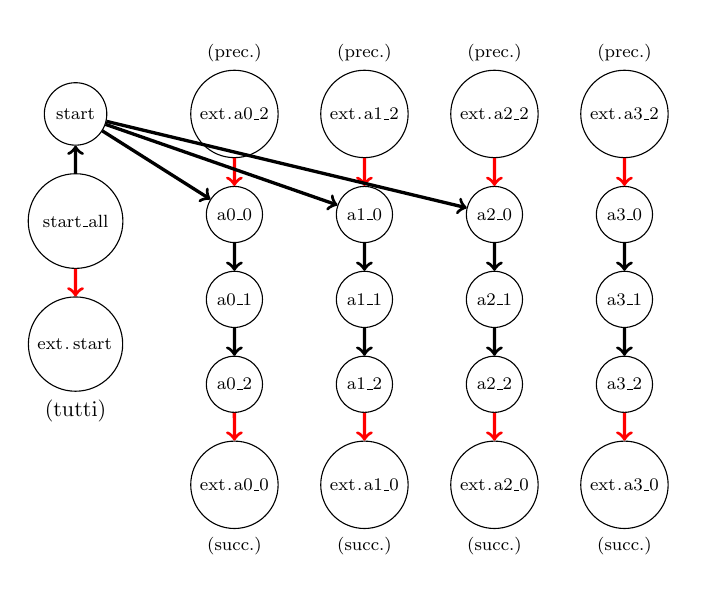
\begin{tikzpicture}[scale=0.8, every node/.style={scale=0.8}]
        \matrix [matrix,row sep=1em,column sep=1.5em,nodes={font=\footnotesize}] {
            %\node[circle, draw](s){$\text{\lstinline{start}}$};           &
            %\node[circle, draw](sa){$\text{\lstinline{start_all}}$};      &
            %\node[circle, draw](ns){$\text{\lstinline{ext.start}}$};
            %\\

            \node[circle, draw, label={above:(prec.)}](pa02){$\text{\lstinline{ext.a0_2}}$}; &
            \node[circle, draw, label={above:(prec.)}](pa12){$\text{\lstinline{ext.a1_2}}$}; &
            \node[circle, draw, label={above:(prec.)}](pa22){$\text{\lstinline{ext.a2_2}}$}; &
            \node[circle, draw, label={above:(prec.)}](pa32){$\text{\lstinline{ext.a3_2}}$};
            \\

            \node[circle, draw](a00){$\text{\lstinline{a0_0}}$};   &
            \node[circle, draw](a10){$\text{\lstinline{a1_0}}$};   &
            \node[circle, draw](a20){$\text{\lstinline{a2_0}}$};   &
            \node[circle, draw](a30){$\text{\lstinline{a3_0}}$}; 
            \\

            \node[circle, draw](a01){$\text{\lstinline{a0_1}}$};   &
            \node[circle, draw](a11){$\text{\lstinline{a1_1}}$};   &
            \node[circle, draw](a21){$\text{\lstinline{a2_1}}$};   &
            \node[circle, draw](a31){$\text{\lstinline{a3_1}}$};  
            \\

            \node[circle, draw](a02){$\text{\lstinline{a0_2}}$};   &
            \node[circle, draw](a12){$\text{\lstinline{a1_2}}$};   &
            \node[circle, draw](a22){$\text{\lstinline{a2_2}}$};   &
            \node[circle, draw](a32){$\text{\lstinline{a3_2}}$};  
            \\

            \node[circle, draw, label={below:(succ.)}](na00){$\text{\lstinline{ext.a0_0}}$}; &
            \node[circle, draw, label={below:(succ.)}](na10){$\text{\lstinline{ext.a1_0}}$}; &
            \node[circle, draw, label={below:(succ.)}](na20){$\text{\lstinline{ext.a2_0}}$}; &
            \node[circle, draw, label={below:(succ.)}](na30){$\text{\lstinline{ext.a3_0}}$};
            \\
        };

        \graph[nodes={font=\footnotesize, circle, draw}]{
            s/\lstinline{start} [left=3em of pa02],
        };

        \graph[nodes={font=\footnotesize, circle, draw}]{
            sa/\lstinline{start_all} [below=1em of s],
        };

        \graph[nodes={font=\footnotesize, circle, draw, label={below:(tutti)}}]{
            ns/\lstinline{ext.start} [below=1em of sa],
        };

        \graph{
            (pa02) -> [draw=red, very thick] (a00) -> [very thick] (a01) -> [very thick] (a02) -> [draw=red, very thick] (na00),
            (pa12) -> [draw=red, very thick] (a10) -> [very thick] (a11) -> [very thick] (a12) -> [draw=red, very thick] (na10),
            (pa22) -> [draw=red, very thick] (a20) -> [very thick] (a21) -> [very thick] (a22) -> [draw=red, very thick] (na20),
            (pa32) -> [draw=red, very thick] (a30) -> [very thick] (a31) -> [very thick] (a32) -> [draw=red, very thick] (na30),
            (s) -> [very thick] (a00),
            (s) -> [very thick] (a10),
            (s) -> [very thick] (a20),
            (sa) -> [very thick] (s),
            (sa) -> [draw=red, very thick] (ns),
        };
    \end{tikzpicture}
    \caption{catene di variabili interne (regole esterne in rosso)}
    \label{fig:interno}
\end{figure}

\begin{figure}[H]
    \centering
    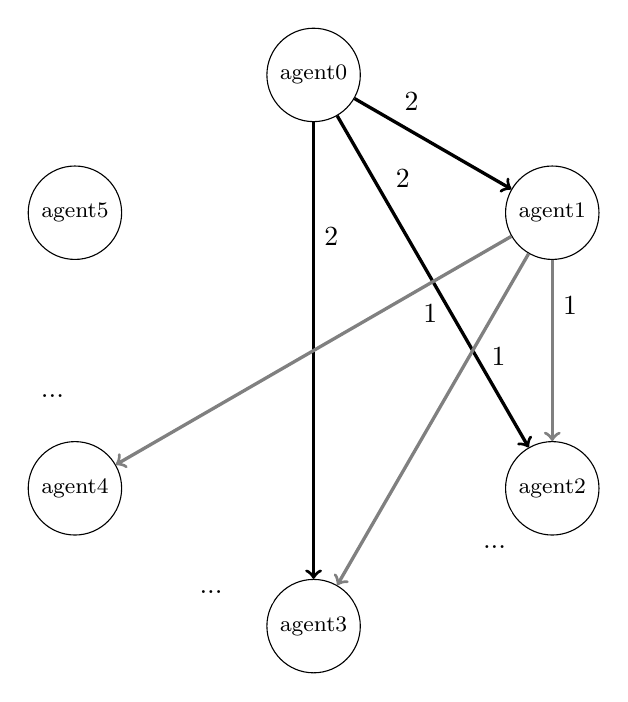
\begin{tikzpicture}
        \graph [clockwise=6,radius=3.5cm,nodes={font=\footnotesize, circle, draw}] {
            a0/agent0,
            a1/agent1,
            a2/agent2,
            a3/agent3,
            a4/agent4,
            a5/agent5,
        };

        \graph {
        (a0) -> [draw=black, edge label=$2$, very thick, near start] (a1),
        (a0) -> [draw=black, edge label=$2$, very thick, near start] (a2),
        (a0) -> [draw=black, edge label=$2$, very thick, near start] (a3),
        (a1) -> [draw=gray, edge label=$1$, very thick, near start] (a2),
        (a1) -> [draw=gray, edge label=$1$, very thick, near start] (a3),
        (a1) -> [draw=gray, edge label=$1$, very thick, near start] (a4),
        (a2) -> [draw=white, edge label=..., very thick, near start] (a3),
        (a3) -> [draw=white, edge label=..., very thick, near start] (a4),
        (a4) -> [draw=white, edge label=..., very thick, near start] (a5),
        };
    \end{tikzpicture}
    \caption{Attivazione dei nodi successivi}
    \label{fig:esterno}
\end{figure}

\paragraph{Struttura delle configurazioni}

Le configurazioni generate con \aeg seguono tutte una stessa struttura, che permette di avviare una computazione che coinvolgerà tutti i nodi e terminerà sempre, i dettagli della configurazione sono controllati da $6$ parametri (interi maggiori di $1$), indicati con $a$, $b$, $c$, $d$, $e$, ed $f$.

Tutti gli $a$ nodi di una configurazione sono simili tra loro: anno le stesse variabili ed eseguono regole uguali, che differiscono al massimo per alcuni valori hardcoded. Ogni nodo ha due variabili booleane \lstinline{start} e \lstinline{start_all} inizializzate a \lstinline{false} che sono usate per avviare una computazione, più $b\times c$ (altro su $b$ e $c$ più avanti) variabili intere con nome \lstinline{ai_j} con $i\in [0,b)$ e $j\in [0,c)$ (e.g.: \lstinline{a0_0}), tutte inizializzate a $0$. Queste variabili rappresentano $b$ ``catene'', ciascuna lunga $c$ variabili, come rappresentato in Figure~\ref{fig:interno}. Ogni nodo ha anche una variabile intera \lstinline{id}, ciascuna inizializzata ad un valore diverso e mai modificata, sono utilizzate solo per indirizzare il singolo nodo.

Ogni dispositivo ha 3 ``regole di avvio'' (rappresentate alla sinistra in Figure~\ref{fig:interno}), una si attiva quando \lstinline{start_all} viene impostato a \lstinline{true}, e non fa altro che impostare la variabile \lstinline{start} a \lstinline{true} su tutti i nodi. Una resetta \lstinline{start_all}. Ed infine quando \lstinline{start} viene impostato a \lstinline{true}, una ``variabile iniziale'' (la variabile \lstinline{ai_0}) delle prime $d\leq b$ catene viene impostata a $f$, e la variabile \lstinline{start} viene resettata. Notare che \lstinline{start_all} non attiva \emph{tutte le catene} (infatti non attiva nessuna catena, ma setta \lstinline{start}), invece attiva le catene di \emph{tutti i nodi}.

Alle prime $c-1$ variabili di ogni catena (quindi da $0$ $c-2$) corrisponde una regola (rappresentate in nero in Figure~\ref{fig:interno}) che si attiva quando la sua variabile viene impostata ad un valore maggiore di $0$, e contemporaneamente copierà il valore della variabile in quella successiva nella catena (e.g.: da \lstinline{a1_2} ad \lstinline{a1_3}) e resetterà la sua variabile.
Quando la $c$-esima variabile dell'$i$-esima catena viene impostata ad un valore $k>0$, non c'è una corrispondente regola ``normale''. Invece ce ne sono una locale che resetta il valore della variabile a $0$, ed una esterna (rappresentate in rosso in fondo a Figure~\ref{fig:interno}) che setterà a $k-1$ il valore della variabile iniziale dell'$i$-esima dei successivi $e$ dispositivi (il dispositivo \lstinline{id} attiva quelli da $((\text{\lstinline{id}}+1)\mod a)$ ad $((\text{\lstinline{id}}+e)\mod a)$). In questo modo la parte di computazione sul dispositivo corrente è completata, e continua sui dispositivi successivi, come visibile in Figure~\ref{fig:esterno}.
Dopo $f$ livelli, il valore che viene passato sulle catene è arrivato ad $1$, e ai prossimi dispositivi viene passato il valore $0$, che le regole del $f+1$-esimo livello di dispositivi ignoreranno.

\paragraph{Parametri di configurazione}

Quindi il comportamento della configurazione è deciso dai (già elencati nella descrizione) parametri:
\begin{itemize}
    \item $a$ (alt.: devices-number) Il numero di nodi nella configurazione
    \item $b$ (alt.: chains-number) Il numero di catene in ogni nodo (non tutte saranno attivate automaticamente)
    \item $c$ (alt.: chain-length) La lunghezza di ogni catena
    \item $d$ (alt.: chain-width) Il numero di catene attivate automaticamente con \lstinline{start=true}
    \item $e$ (alt.: devices-width) Il numero di dispositivi attivati al termine di una catena
    \item $f$ (alt.: devices-length) Il numero di livelli attraversati prima di arrivare a $0$
\end{itemize}

Oltre a questi 6 parametri di configurazione, se ne possono impostare anche alcuni riguardanti il setting dell'esperimento, come l'immagine Docker da usare per i nodi ed il coordinatore, oppure il tick.
Per questa tesi sono rilevanti solo i 6 parametri di configurazione, in quanto il setting sperimentale (tempo di tick, immagini Docker, etc.) è rimasto lo stesso in ogni test.

\section{Terminazione forte}
% Non sono sicuro che basti come dimostrazione, spero di sì perché non è stata facile da scrivere

Per semplicità affronteremo la terminazione in due parti. La prima parte riguarda solo la parte ``interna'' della computazione, quella che si occupa di trasportare i valori nelle catene di variabili, ignorando i valori che potrebbero essere aggiunti da una regola esterna avviata da un altro nodo.
E la seconda riguardante solo i dispositivi che vengono attivati dalle regole esterne, assumendo che la parte interna termini correttamente, attivando i nodi successivi.
Sarebbe possibile fornire una dimostrazione unica che tratti direttamente entrambe le parti della computazione, ma è molto più difficile.

\paragraph{Stabilizzazione interna}

La terminazione sarà dimostrata prima in maniera meno formale, considerando un sistema in cui la regola da eseguire viene scelta dando la precedenza quelle che scrivono le variabili più vicine alla fine di una catena, e dando la precedenza alle catene con indice più alto. Questo permette di fissare l'ordine di esecuzione delle regole in uno su cui è più comodo ragionare. E infine sarà accennato perché un ordine così stringente non è necessario.
Inoltre assumeremo, come annunciato ad inizio sezione, che nessun nodo esterno imposti il valore di alcuna variabile, tuttavia in seguito spiegheremo perché non sia un problema nel paragrafo sulla convergenza totale.

Sia $(a_{0,0},...,a_{0,c-1},a_{1,0},...,a_{1,c-1},...,a_{b-1,c-1})\in \mathbb{N}^{bc}$ il vettore che rappresenta lo stato interno di un generico nodo della configurazione (ogni variabile $a_{i,j}$ rappresenta la variabile \lstinline{ai_j}). È facile verificare che ogni regola normale viene attivata da uno stato del tipo $(...,a_{i,j},a_{i,j+1},...)$ e causa uno stato del tipo $(...,0,a_{i,j},...)$ (notare che l'indice della catena è sempre $i$) e causerà l'inserimento di una nuova regola nella coda degli eventi.
Ricordiamo che con l'ordinamento stabilito ad inizio paragrafo, la regola attivata dallo stato $(...,a_{i,j},a_{i,j+1},...)$ verrà eseguita solo quando $a_{i,j+1}=0$, altrimenti ci sarebbe una regola con precedenza più alta.
Una regola finale, invece è causata da uno stato del tipo $(...,a_{i,j},a_{i+1,0},...)$ e ne causa uno del tipo $(...,0,a_{i+1,0},...)$ senza causare nessun inserimento.

Sapendo che: la computazione termina se e solo se il vettore che rappresenta lo stato interno è $(0,...,0)$, altrimenti ci sarebbero ancora regole in coda, attivate quando sono state impostate le variabili diverse da $0$; e che ogni regola causa uno stato di ordine lessicografico minore rispetto a quello che lo ha attivato; possiamo concludere che la computazione deve terminare per forza altrimenti potrebbe scendere di ordine lessicografico all'infinito.
Ed al termine di questa computazione, saranno state eseguite le regole esterne per attivare i nodi successivi, perché le uniche regole che non aggiungono nuove regole sono attivate dallo stesso stato che causa l'attivazione delle regole esterne.

AbU, per sua natura, non fa garanzie sull'ordine di esecuzione delle regole causate dallo stesso stato, quindi per completare la dimostrazione formale dobbiamo mostrare che funzionerebbe anche senza questo ordinamento.
Possiamo vedere che non importa perché: esiste una corrispondenza diretta tra le variabili e le regole, e non ci sono ``interferenze'' tra le regole causate dallo stesso stato (non cercano di leggere la stessa variabile o di scrivere la stessa), ed è sufficiente entrare una volta in uno stato ed uscirne subito per attivare una regola.
Quindi l'ordine non importa, e quindi la computazione interna termina sempre.

\paragraph{Stabilizzazione esterna}

Come annunciato all'inizio della sezione, affronteremo la stabilizzazione esterna considerando corretta la parte interna della computazione. Ovvero assumendo che nodo che viene ``attivato'' da un valore $k$, eventualmente attiverà $e$ nodi con un valore $k-1$. Questo segue dalla dimostrazione precedente.

Consideriamo l'attivazione di un nodo come il passaggio di un token, ogni token ha un'``intensità'' $k$, ovvero il numero di livelli che può attraversare. Quando un nodo elabora un token, questo viene spezzato in $e$ token di intensità $k-1$, e quando un token ha intensità $0$, il nodo che lo riceve lo scarta.
Nelle nostre computazioni, l'intensità del token corrisponde al valore $k$ con cui il nodo viene attivato, ovvero il valore che la regola finale esterna inserisce all'inizio della catena di variabili dei nodi successivi. Quando viene impostata \lstinline{start = true} su di un nodo, questo genera $b$ token di intensità $f$. Quando viene impostata \lstinline{start_all = true} su un qualsiasi nodo, tutti gli $a$ nodi generano $b$ token ciascuno di intensità $f$.

Sia $(t_f,t_{f-1},...,t_1)\in\mathbb{N}^f$ il vettore dei token, dove ogni variabile $t_k$ rappresenta la quantità di token di intensità $k$ in circolazione sulla rete. Notiamo che i token di intensità $0$ non vengono contati, perché sono scartati subito.
Possiamo osservare che ogni volta che un token di intensità $k$ viene consumato, il vettore passa da $(...,t_k,t_{k-1},...)$ a $(...,t_k-1,t_{k-1}+e,...)$. Quindi ad ogni consumo, il nuovo vettore ha ordine lessicografico più basso di quello iniziale.

Sapendo che la computazione esterna si ferma se e solo se non ci sono più token in circolazione, quindi il vettore ha valore $(0,...,0)$, e che ad ogni avanzamento della computazione l'ordine lessicografico scende, sappiamo che la computazione deve terminare per forza.

Ammettendo che più token vengano consumati contemporaneamente, il risultato non cambia, perché si passerebbe comunque ad uno vettore più in basso nell'ordine lessicografico.

\paragraph{Stabilizzazione totale}

Per mettere insieme i due risultati manca solo dimostrare che ammettere attivazioni esterne non impedisce la stabilizzazione interna. Riuscendo a dimostrare questo, avremmo che internamente la computazione termina in ogni caso, ed esternamente termina se quella interna termina.

Dimostrare questa non interferenza è facile utilizzando lo stesso ordine rigido che abbiamo usato per rendere più breve la dimostrazione della stabilizzazione interna. Con quell'ordine rigido, le regole esterne che attiverebbero il nodo catena non verrebbero mai selezionate per prime per l'esecuzione, perché scrivono sulle variabili più lontane dalla fine della catena.
In questo modo, il nodo comincerebbe ad eseguire le regole di attivazione solo dopo aver terminato la computazione interna già in corso. Quindi l'attivazione non interferirebbe con la stabilizzazione.

Ovviamente AbU non prevede questo ordinamento, ma come spiegato nel paragrafo sulla stabilizzazione interna, imporre questo ordinamento non influisce sul comportamento della nostra computazione.

\section{Scelta delle configurazioni}

Per l'analisi di GoAbU sono stati scelti tre casi di test di base, e poi ogni caso è stato testato con $10$, $50$ e $100$ nodi, ciascuno dei tre vuole mettere in evidenza diversi aspetti di AbU.

In tutti i casi, l'unico dato che ci importava raccogliere erano le informazioni sul traffico di rete. Nella prossima sezione ~\ref{raccolta:quali} spiegheremo perché questa scelta.

\paragraph{Idle}

Il primo caso non prevede nessuna regola, il sistema è composto solo da nodi ``vuoti'' ed i test in questo caso (a contrario degli altri due) sono stati condotti senza avviare mai la computazione.
L'obbiettivo è quello di osservare il comportamento dell'implementazione quando non succede nulla, verificare la presenza di overhead o di un ``rumore di fondo'' da poter rimuovere dai test successivi.

In particolare ci interessava il traffico causato dal middleware memberlist per mantenere la comunicazione di gruppo attiva anche senza nessuna transazione.

Questo test serve per scoprire se un sistema con tanti nodi sia impraticabile a prescindere dal tipo di lavoro che svolgono. Se mantenere i nodi connessi causa già troppo traffico per poter utilizzare GoAbU in una rete vera, bisognerebbe cambiare completamente l'implementazione.

\begin{itemize}
    \item $a=10|50|100$
    \item $b=1$
    \item $c=1$
    \item $d=1$
    \item $e=1$
    \item $f=1$
\end{itemize}

\paragraph{Medio}

Progettando questo test l'obbiettivo era quello di ricreare un test che anche se esigente, fosse in qualche modo realistico, un test in cui ogni nodo ha una certa quantità di regole, ed alcune (non tutte) di queste si attivano. Ed una frazione di queste causano degli effetti su un solo altro nodo (non troppi).

L'obbiettivo era non essere troppo pesante sulla rete, ma bilanciare il carico tra rete e nodo interno. In un certo tempo, ogni nodo avrà molte più regole locali di cui occuparsi, e dovrebbe utilizzare di meno la rete.

Questo test, come anche il successivo, è stato progettato in modo che richieda $\qty{500}{\second}$ per terminare la computazione. Ed effettivamente con pochi dispositivi è così, ma in realtà l'overhead dell'esecuzione del rule engine, e soprattutto quello della rete, fanno sì che in realtà richieda più tempo.
Il tempo reale e dipendente dal setting sperimentale, quindi dalla macchina che esegue il simulatore, e non direttamente da GoAbU. Tuttavia, il fatto che con $100$ dispositivi la macchina sia in difficoltà, significa che potrebbero esserlo anche i dispositivi di rete.

In ogni caso, abbiamo osservato che il tempo di esecuzione è molto consistente tra le ripetizioni della computazione. Quindi dopo aver provato una volta ad eseguire una computazione con un certo numero di nodi, possiamo assumere che la prossima impieghi un tempo molto simile.

\begin{itemize}
    \item $a=10|50|100$
    \item $b=10$
    \item $c=5$
    \item $d=5$
    \item $e=1$
    \item $f=20$
\end{itemize}

\begin{tabular}{| c | c | c |}
    \hline
    \multirow{2}{*}{Nodi} & \multicolumn{2}{c |}{ Regole }           \\
    \cline{2-3}
                            & Interne                        & Esterne \\
    \hline\hline
    $10$                  & $5000$                         & $1000$  \\
    \hline
    $50$                  & $25000$                        & $5000$  \\
    \hline
    $100$                 & $50000$                        & $10000$ \\
    \hline
\end{tabular}\label{tab:medio}

\paragraph{Alto}

L'ultimo test è stato progettato con l'obbiettivo esplicito di mettere in difficoltà la rete quanto più possibile in un tempo limitato. Come si vede dalla configurazione, sono presenti molte meno regole interne rispetto a quelle esterne.
Invece ogni dispositivo attiva direttamente altri $3$ dispositivi e si prosegue in $5$ livelli di profondità. In questo modo il numero di messaggi inviati nella rete cresce in modo quasi esponenzialmente nel tempo.

Questo test è stato costruito in cercando una combinazione di $e$ ed $f$ tali che con pochi dispositivi la computazione termini in $\qty{500}{\second}$. Però il carico è molto alto e quando si arriva a 100 dispositivi, la computazione viene completata in $\qty{2000}{\second}$.
Come detto in precedenza, questo tempo non è significativo poiché dipende principalmente dalla macchina su cui viene eseguito il simulatore. Però una differenza del genere suggerisce che anche il traffico di rete sarà particolarmente alto.

\begin{itemize}
    \item $a=10|50|100$
    \item $b=1$
    \item $c=1$
    \item $d=1$
    \item $e=3$
    \item $f=5$
\end{itemize}

\begin{tabular}{| c | c | c |}
    \hline
    \multirow{2}{*}{Nodi} & \multicolumn{2}{c |}{ Regole }           \\
    \cline{2-3}
                            & Interne                        & Esterne \\
    \hline\hline
    $10$                  & $1210$                         & $3630$  \\
    \hline
    $50$                  & $6050$                         & $18150$ \\
    \hline
    $100$                 & $12100$                        & $36300$ \\
    \hline
\end{tabular}\label{tab:alto}

\chapter{Raccolta dati}\label{raccolta}

\section{Quali dati raccogliere}\label{raccolta:quali}

Prima di affrontare qualsiasi tipo di test bisogna stabilire quali sono i dati che importano e come raccoglierli in modo efficace.
In un sistema distribuito sono tanti gli aspetti che si potrebbero prendere in considerazione. Traffico di rete, latenza dell'esecuzione delle regole, throughput dei singoli nodi, throughput dell'intero sistema. Tutte queste opzioni sono state considerate prima di scegliere che test eseguire.

AbU non è pensato per svolgere calcoli, ma per sincronizzare dispositivi.
Quindi in un'applicazione reale non c'è un vero risultato in output, un qualcosa di cui misurare il throughput. Al massimo si possono misurare la quantità di regole eseguite, ma quelle sono legate al tick che è impostato manualmente.

La latenza delle regole anzitutto dipende più dal numero totale di regole, e dalle prestazioni del dispositivo che esegue GoAbU, che da GoAbU stesso, quindi anche questa metrica non è molto indicativa delle prestazioni.
In ogni caso, per migliorarla bisognerebbe passare ad un rule engine più ``aggressivo'', o trovare un modo di utilizzare meno regole.
In ogni caso, il tempo speso per attendere il passare del tick è molto più lungo della latenza di una regola, a meno che la knowledge base non sia enorme.
Quindi anche questo dato è stato considerato non necessario, almeno per ora.

Alla fine, abbiamo deciso di raccogliere solo i dati relativi al traffico di rete. Più precisamente abbiamo raccolto sia la dimensione totale dei messaggi inviati e ricevuti (come numero di byte totali), che la quantità di pacchetti (frame di livello 2) inviati e ricevuti. Entrambi questi dati sono reperibili direttamente dal sistema operativo.
Inoltre, abbiamo deciso di raccogliere anche il numero di messaggi inviati a livello di libreria, e la dimensione di questi messaggi. Per poterle confrontare con i dati del sistema operativo e scoprire quando overhead viene aggiunto dal middleware.
Queste ultime informazioni sono state raccolte solo per gli ultimi due casi, quello medio e quello alto, perché in idle la libreria non produce azioni.

\section{Ispezione dei nodi}

Le informazioni sul traffico di rete sono fornite direttamente dal sistema operativo, che offre degli pseudo-file per processo dove sono listate diverse metriche (in particolare byte e pacchetti, inviati e ricevuti) per ogni interfaccia di rete, utilizzate fino a quel momento dal processo.

Come già visto in precedenza~\ref{setting:abusim} AbUsim utilizza due reti virtuali (quindi ogni nodo ha due interfacce di rete), una utilizzata per la comunicazione di GoAbU, ed una per il resto delle funzioni del simulatore, come l'invio dei log.
Quindi è facile ottenere solo i dati riguardanti GoAbU senza che siano influenzati dal simulatore. È sufficiente identificare prima l'interfaccia di rete utilizzata per GoAbU, sempre usando gli pseudo-file, e poi raccogliere solo le metriche di quell'interfaccia.

Per separare i dati riguardanti una computazione da quelli precedente e da quelli della discovery, raccogliamo i dati prima e dopo la computazione, ed teniamo la differenza.

I dati sui messaggi, invece, sono raccolte tramite i log del simulatore, che sono stati modificati appositamente per includere questi dati.
Purtroppo, per quanto riguarda i messaggi, abbiamo raccolto i log di un solo nodo poiché le dimensioni erano troppo grandi. Raccogliendo i dati di un solo nodo sono stati prodotti $\qty{230}{\mebi\byte}$ di file di log, quindi raccoglierli per tutti i nodi sarebbe stato dispendioso.
In futuro, si potrebbe trovare un modo per fornire questi dati in modo più snello, per poter analizzare più nodi.

\section{Metriche}

Elenchiamo tutte le metriche ottenute, con una breve descrizione

\begin{itemize}
    \item \lstinline{received bytes}: Indica il numero totale di byte ricevuti da un agente in un test
    \item \lstinline{received packets}: Indica il numero totale di pacchetti ricevuti da un agente in un test
    \item \lstinline{sent bytes}: Indica il numero totale di byte inviati da un agente in un test
    \item \lstinline{sent packets}: Indica il numero totale di pacchetti inviati da un agente in un test
    \item \lstinline{received bytes per seconds}: Come sopra, ma diviso per la durata del test
    \item \lstinline{received packets per seconds}: Come sopra, ma diviso per la durata del test
    \item \lstinline{sent bytes per seconds}: Come sopra, ma diviso per la durata del test
    \item \lstinline{sent packets per seconds}: Come sopra, ma diviso per la durata del test
    \item \lstinline{bytes ratio}: Rapporto tra byte ricevuti ed inviati
    \item \lstinline{packets ratio}: Rapporto tra pacchetti ricevuti ed inviati
    \item \lstinline{bytes per packet}: Dimensione in byte dei pacchetti
    \item \lstinline{total bytes}: Byte inviati in totale nella rete
    \item \lstinline{total packets}: Pacchetti inviati in totale nella rete
    \item \lstinline{total bytes per seconds}: Come sopra, ma diviso per la durata del test
    \item \lstinline{total packets per seconds}: Come sopra, ma diviso per la durata del test
    \item \lstinline{logs_expected bytes}: Dimensione totale dei messaggi riportata nei log
    \item \lstinline{logs_actual bytes}: Byte effettivamente inviati dal nodo loggato
    \item \lstinline{logs_expected packets}: Numero di messaggi riportati nei log
    \item \lstinline{logs_actual packets}: Pacchetti effettivamente inviati dal nodo loggato
    \item \lstinline{logs_bytes ratio}: Rapporto tra bytes effettivamente inviati e quelli riportati nel log
    \item \lstinline{logs_packets ratio}: Rapporto tra pacchetti inviati e messaggi riportati nel log
\end{itemize}

Le metriche riguardanti il tempo sono state raccolte, ma non sono rilevanti, perché il tempo dipende principalmente dal tick, e nel nostro caso anche dalla macchina che esegue il simulatore. Quindi non verranno analizzati.

Le metriche riguardanti il traffico ricevuto, sono interessanti, ma non particolarmente utili. Ogni dato ricevuto è un nodo che era stato inviato da un altro nodo, quindi i dati inviati in totale e quelli ricevuti dovrebbero essere simili.
Dal rapporto possiamo ottenere il packet loss della rete, però questo non fornisce nessuna informazione sul comportamento di GoAbU, ma sul comportamento delle reti Docker.

I dati sui pacchetti di livello 2 sono interessanti in quanto sono indicativi del lavoro che dovranno gestire i dispositivi di rete a cui AbU sarà connesso.

Confrontare i dati del sistema con quelli dei log permette di osservare cosa il middleware è in grado di fare per ridurre il traffico. In particolare, i due rapporti \lstinline{logs_bytes ratio} e \lstinline{logs_packets ratio} facilitano questo confronto.
Più precisamente, il primo mette in evidenza la capacità del middleware di comprimere ed ottimizzare i dati.
Il secondo invece mette in evidenza quanti pacchetti servono per un messaggio.

Oltre a questo, le metriche totali, quindi \lstinline{total bytes} e \lstinline{total packets}, forniscono una misura complessiva del traffico, quindi la quantità di byte e pacchetti, che attraversa la rete da parte di tutti i nodi.
Questo è uno dei dati più importanti, perché potrebbe essere il fattore più limitante in una rete reale. Se il data-rate fosse una limitazione, sarebbe sufficiente allungare il tick dei nodi che generano più traffico, ma la quantità totale di dati resta la stessa.

Bisogna notare che i pacchetti sono di livello 2, quindi oltre a quelli causati da GoAbU sono inclusi anche altri protocolli ancillari IP e le richieste ARP, perché il sistema non li separa.
Per quanto sarebbe interessante avere un dato più preciso, questi pacchetti ``non GoAbU'' non saranno molti se paragonati a quelli di GoAbU. Inoltre, si tratta di un dato più indicativo dello stress che viene messo sulla rete, in particolare sugli switch ed access point.

\chapter{Risultati}\label{risultati}

\section{Grafici}

\paragraph{\lstinline{total bytes}}

\begin{figure}[H]
    \centering
    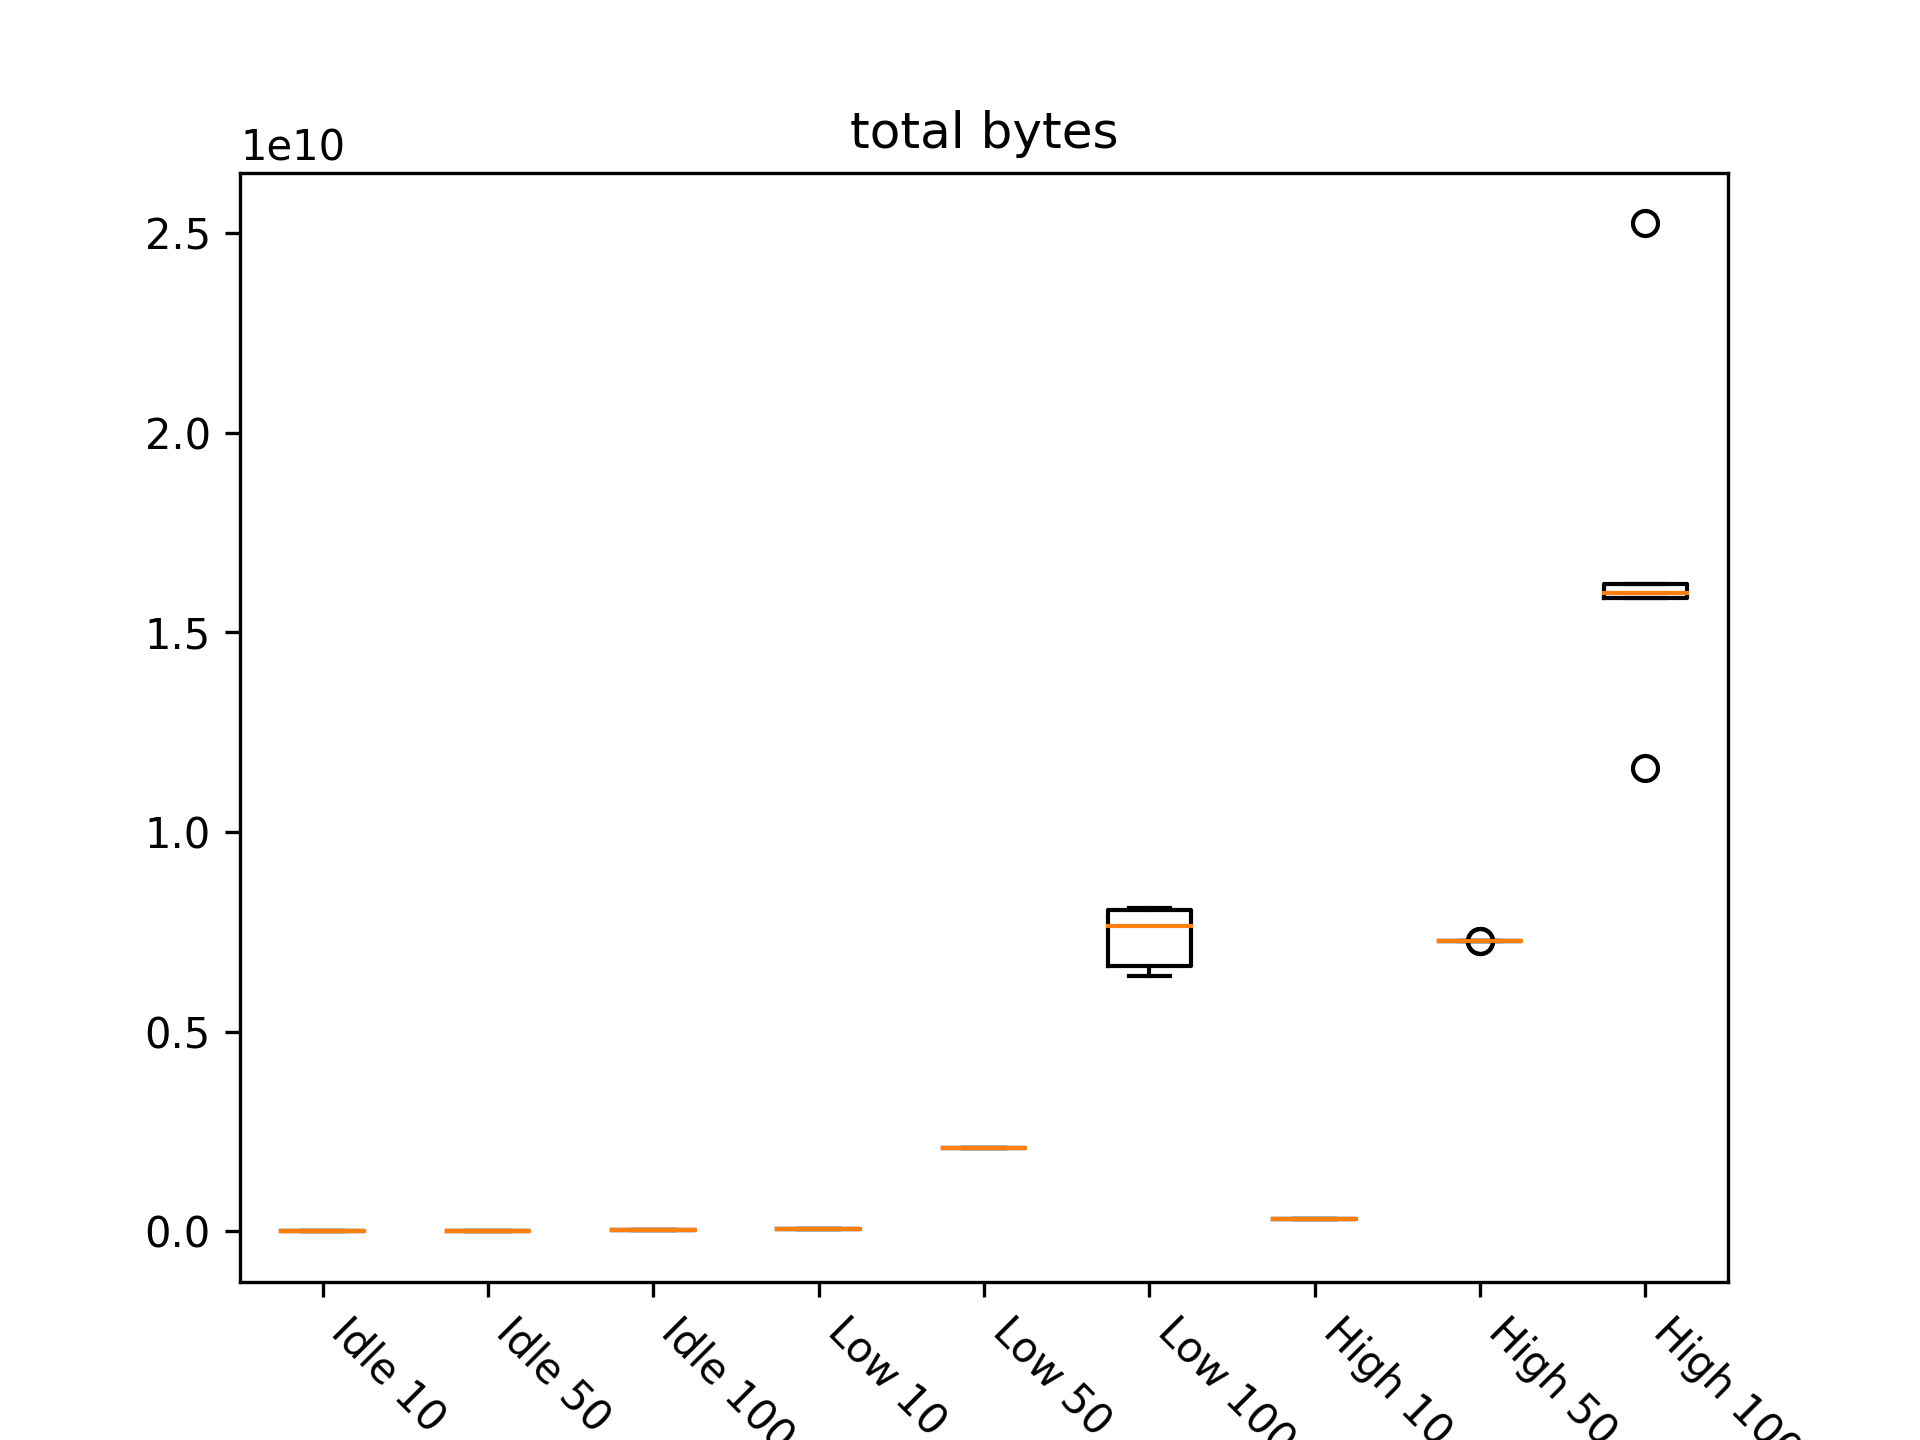
\includegraphics[width=0.7\linewidth, keepaspectratio]{graphs/total bytes.png}
    \caption{Byte inviati in totale nella rete}
    \label{fig:tb}
\end{figure}

In questo grafico possiamo osservare il traffico totale che attraversa la rete, in byte.

Notiamo anzitutto che in idle il traffico è molto basso, come ci si aspetta. Significa quindi che il middleware non ha bisogno di grandi scambi di dati per mantenere la comunicazione di gruppo ed il gossiping.
All'aumentare dei nodi passa da $\sim\qty{2}{\mega\byte}$ a $\sim\qty{9}{\mega\byte}$, a $\sim\qty{20}{\mega\byte}$, di traffico, l'aumento sembra approssimativamente lineare rispetto al numero di nodi.
I test in idle sono gli unici dove ha senso guardare le metriche al secondo, e si tratta di pochi $\unit{\kilo\byte/\second}$ (grafico in appendice, Figure~\ref{fig:tbps}).

I risultati per i test sotto carico medio sono molto meno promettenti. Già con $10$ nodi, i valori sono ben oltre il carico in idle per $100$ nodi, con $\sim\qty{62}{\mega\byte}$ di dati.\\
Più preoccupante è il salto tra i $50$ ed i $100$ nodi, in cui il traffico passa da $\sim\qty{208}{\mega\byte}$ a $\sim\qty{7.4}{\giga\byte}$. L'aumento non sembra affatto lineare, ma non siamo sorpresi, perché implementando il broadcast come messaggi unicast ad ogni nodo, ci \emph{aspettiamo} una message complexity di $\Theta(a^2)$.

I risultati per i test sotto carico alto sono pessimi. Ci aspettavamo di vedere un traffico molto alto, però un traffico di $\sim\qty{302}{\mega\byte}$ con soli $10$ nodi, rende AbU inadatto all'utilizzo in una rete realistica per problemi così pesanti sulla rete.
Ovviamente si tratta di un benchmark con un carico estremo e poco realistico già per cominciare, ma AbU vuole essere utilizzabile anche in sistemi molto grandi.

Inaspettatamente, all'aumentare dei nodi passa a $\sim\qty{7.3}{\giga\byte}$ e poi $\sim\qty{16}{\giga\byte}$, che \emph{sembra} molto più vicina ad una crescita lineare rispetto a quella del carico medio.
Per indagare ulteriormente su questo risultato inaspettato. Considerando anche il traffico per regola esterna otteniamo:

\begin{tabular}{| c | c |}
    \hline
    Test                          & $\unit{\kilo\byte/rule}$ \\
    \hline
    $\text{\lstinline{low 10}}$   & $\sim62$                 \\
    \hline
    $\text{\lstinline{low 50}}$   & $\sim104$                \\
    \hline
    $\text{\lstinline{low 100}}$  & $\sim736$                \\
    \hline
    $\text{\lstinline{high 10}}$  & $\sim83$                 \\
    \hline
    $\text{\lstinline{high 50}}$  & $\sim401$                \\
    \hline
    $\text{\lstinline{high 100}}$ & $\sim467$                \\
    \hline
\end{tabular}\label{tab:bpr}

Notiamo che, per $10$ e soprattutto $50$ nodi, il traffico per regola causato dal carico alto è molto maggiore di quello sotto carico medio.
Con $100$ nodi, invece, il traffico per regola sotto carico alto è molto più vicino al caso con $50$ nodi e molto più basso ($\sim\qty{36.7}{\percent}$ in meno) del traffico per regola sotto carico medio.
Sembra che ad un certo punto aumentare le regole cominci a ridurre i costi per la singola regola.

Nonostante questo risultato promettente, c'è un outlier del test con $100$ nodi che ha prodotto $\sim\qty{25}{\giga\byte}$ di traffico, significa che in determinate condizioni potrebbe causare molto più traffico.
Il traffico per regola in quel caso è di $\qty{689}{\percent}$, che è comunque più basso del test sotto carico medio.
Ad ogni modo, anche se la singola regola è meno costosa, nel complesso i dati passati nella rete sono aumentati di molto.

\paragraph{\lstinline{total packets}}

\begin{figure}[H]
    \centering
    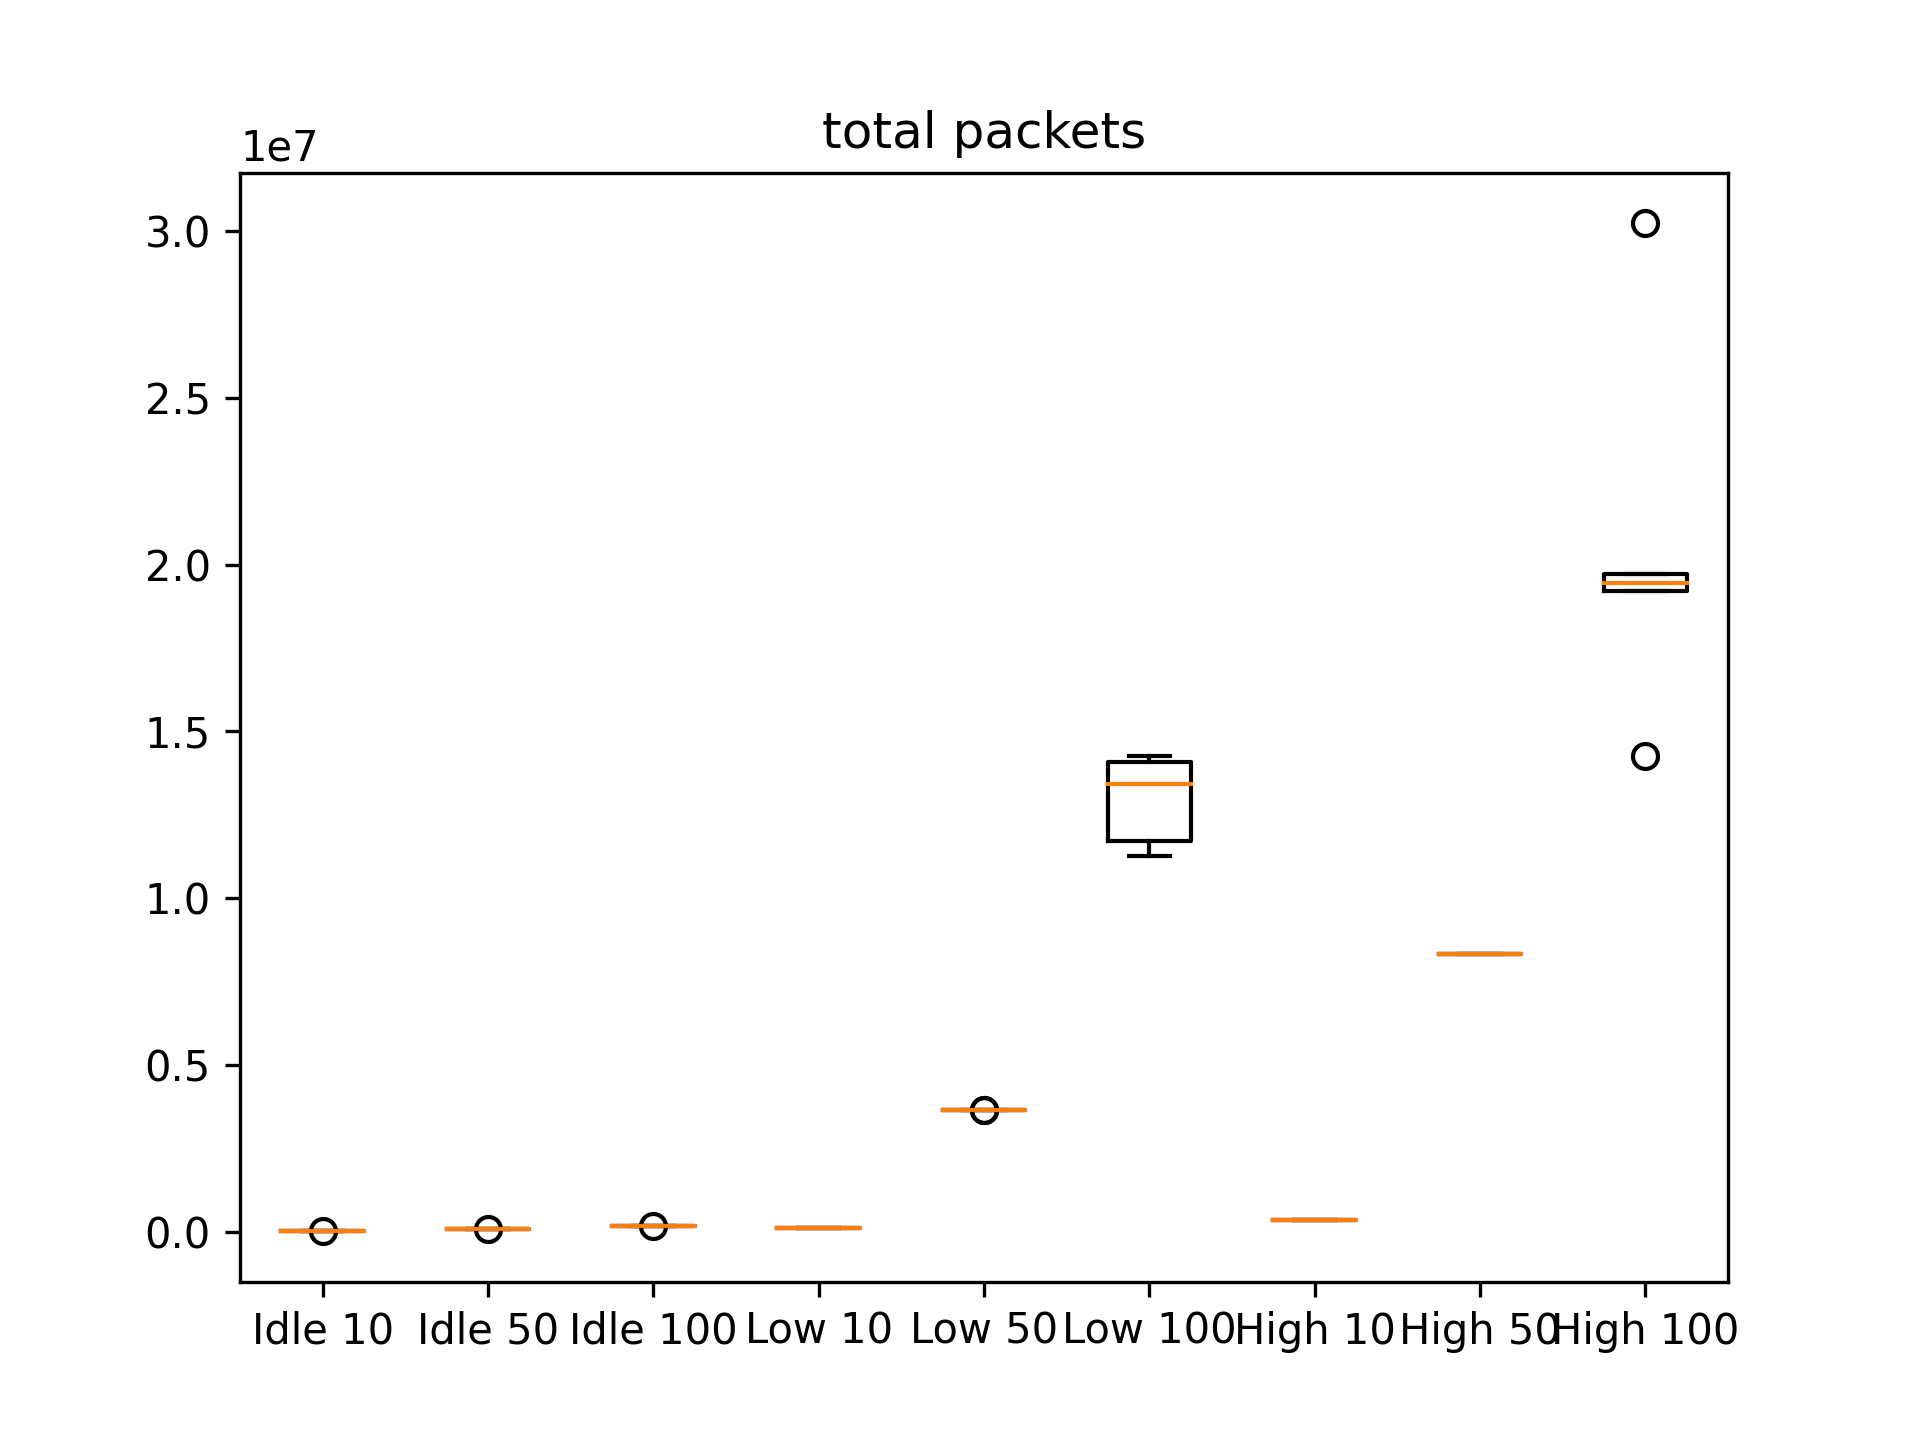
\includegraphics[width=0.7\linewidth, keepaspectratio]{graphs/total packets.png}
    \caption{Pacchetti inviati in totale nella rete}
    \label{fig:tp}
\end{figure}

Questo grafico, per i test sotto carico medio ed alto, non fornisce particolari informazioni oltre a quelle messe in evidenza dal grafico \lstinline{total bytes} Figure~\ref{fig:tb}.

Dai pacchetti risulta chiaro che la message complexity (stavolta come numero di pacchetti e non dimensione) non sia lineare. Infatti, il numero di pacchetti nei test con $100$ nodi è anche $100$ volte più grande di quello nei test con $10$ nodi, mentre con $50$ nodi è $30$ volte più grande.

Per i test in idle, a contrario di quanto visto nel grafico precedente, anche senza carico, il numero di pacchetti cresce in modo non lineare, ma comunque meno di come cresce sotto carico. In seguito vedremo altri dati su questo argomento quando parleremo del grafico \lstinline{bytes per packets} Figure~\ref{fig:bp}.

\paragraph{\lstinline{logs_bytes ratio}}

\begin{figure}[H]
    \centering
    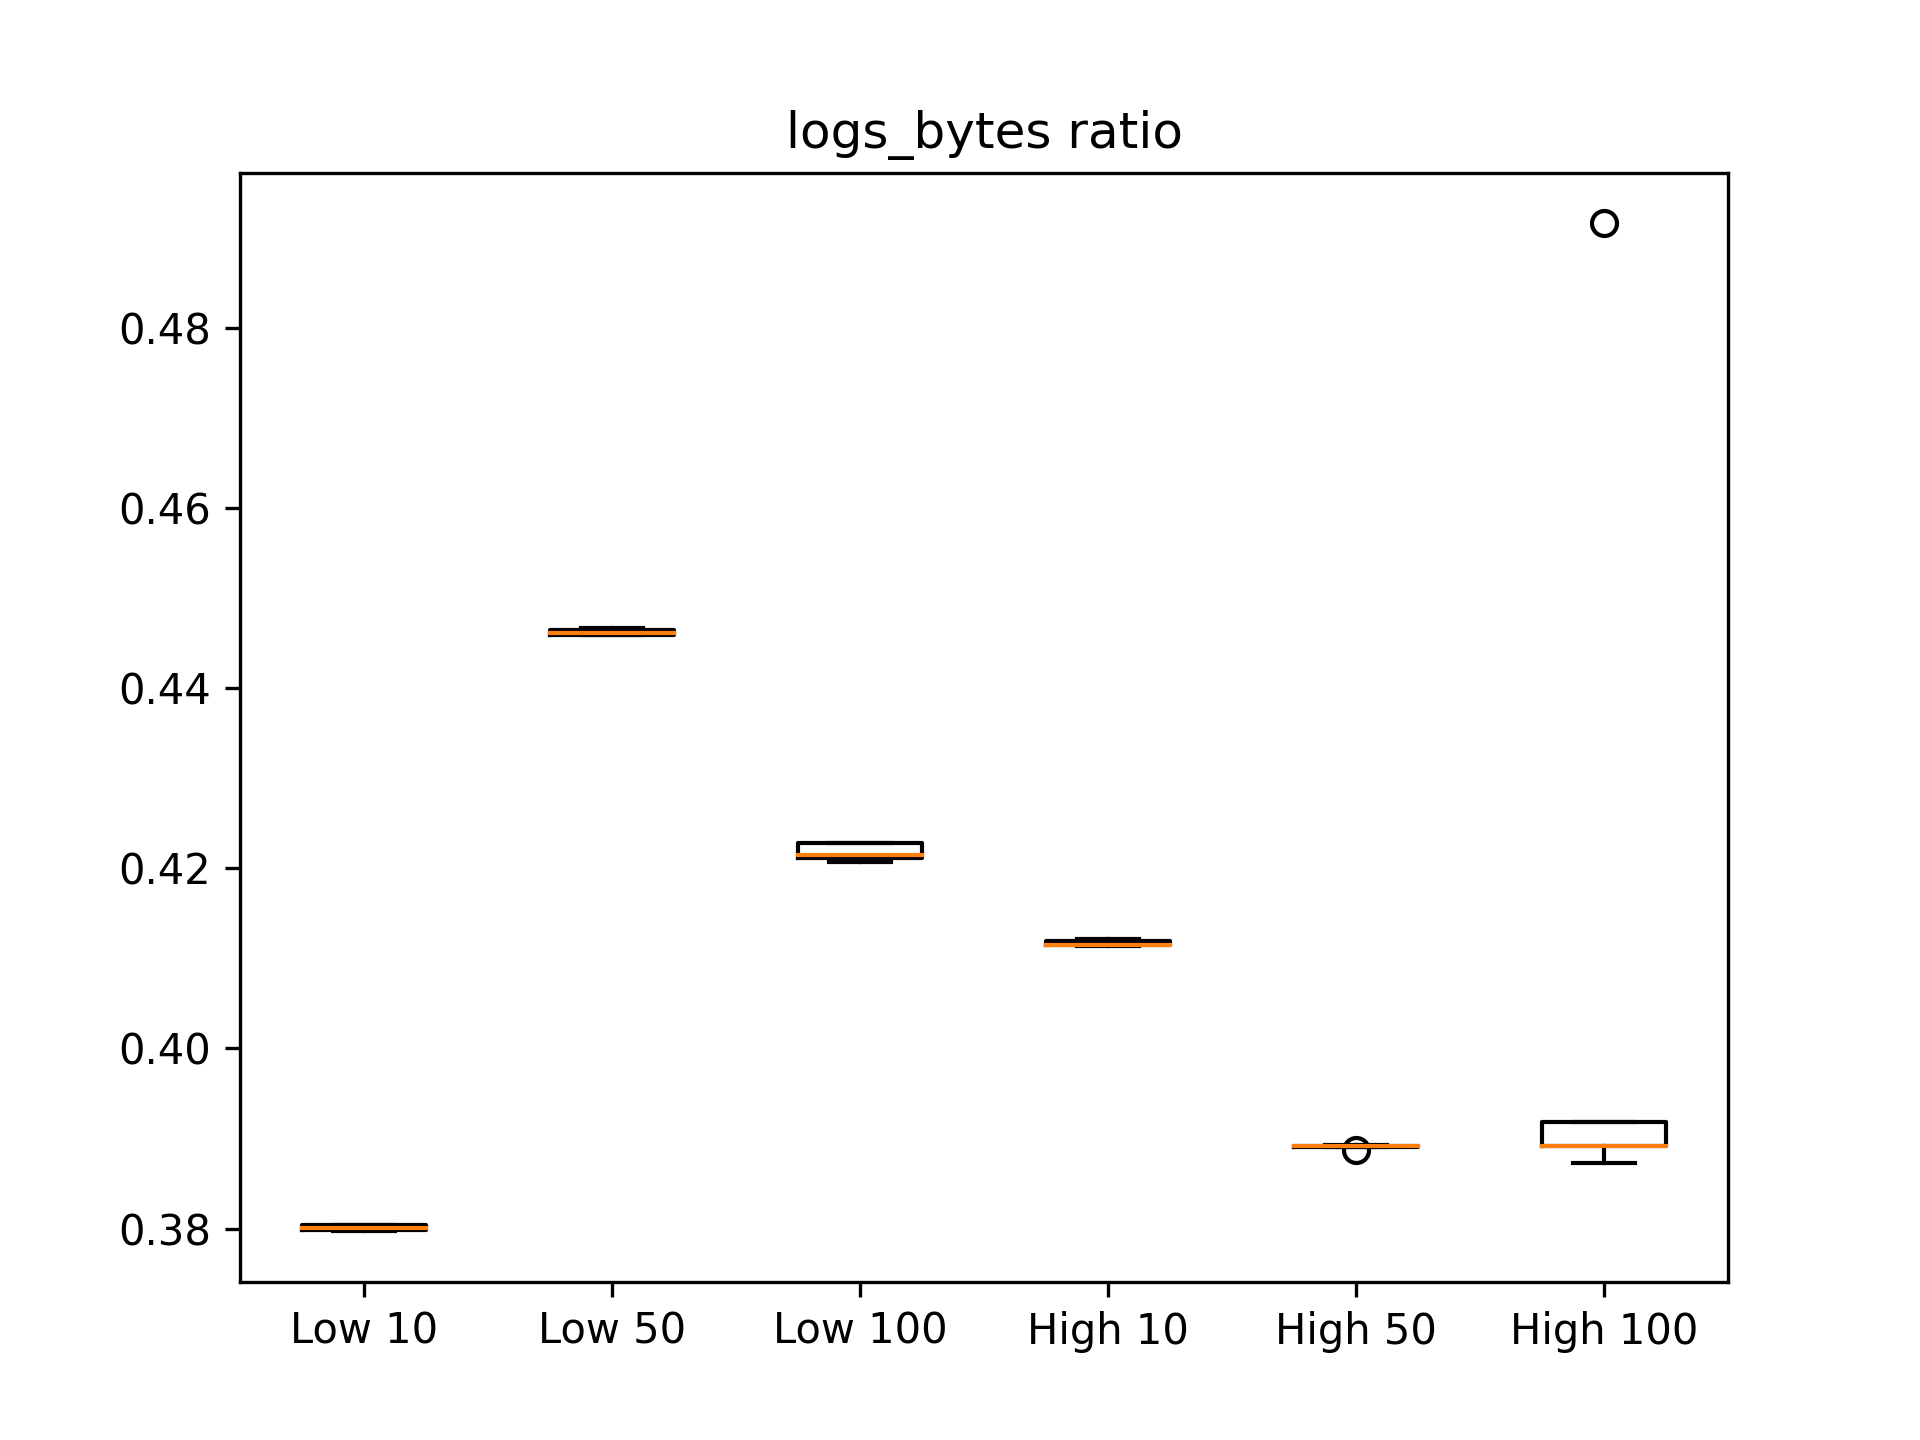
\includegraphics[width=0.7\linewidth, keepaspectratio]{graphs/logs_bytes ratio.png}
    \caption{Rapporto tra bytes effettivamente inviati e quelli riportati nel log}
    \label{fig:lbr}
\end{figure}

In questo grafico possiamo osservare se l'utilizzo del middleware memberlist causa overhead o comprime i dati in modo osservabile.
È calcolato confrontando la quantità byte dati inviati riportata dal sistema, con la somma della dimensione di tutti i messaggi eseguite a dalla libreria. Quindi un valore maggiore di $1$ indica un complessivo overhead, mentre un valore minore di $1$ indica una compressione migliore.

Possiamo osservare dai rapporti con valori da $0.38$ a $0.46$, che la compressione riesce a rendere i dati da inviare meno della metà dei dati di partenza.
Il rapporto di compressione è tra il $2.2$ ed il $2.6$, che è molto alto.

Come già visto nella Sezione~\ref{setting}, il corpo dei è una serializzazione \lstinline{json} che contiene l'albero sintattico della regola codificata in \lstinline{base64}.
La stringa risultante, passata al middleware per l'invio è molto lunga, ma avendo poche informazioni (relativamente alla lunghezza) ci aspettiamo che abbia poca entropia, e che per questo possa essere compressa così tanto, così facilmente.

\paragraph{\lstinline{logs_packets ratio}}

\begin{figure}[H]
    \centering
    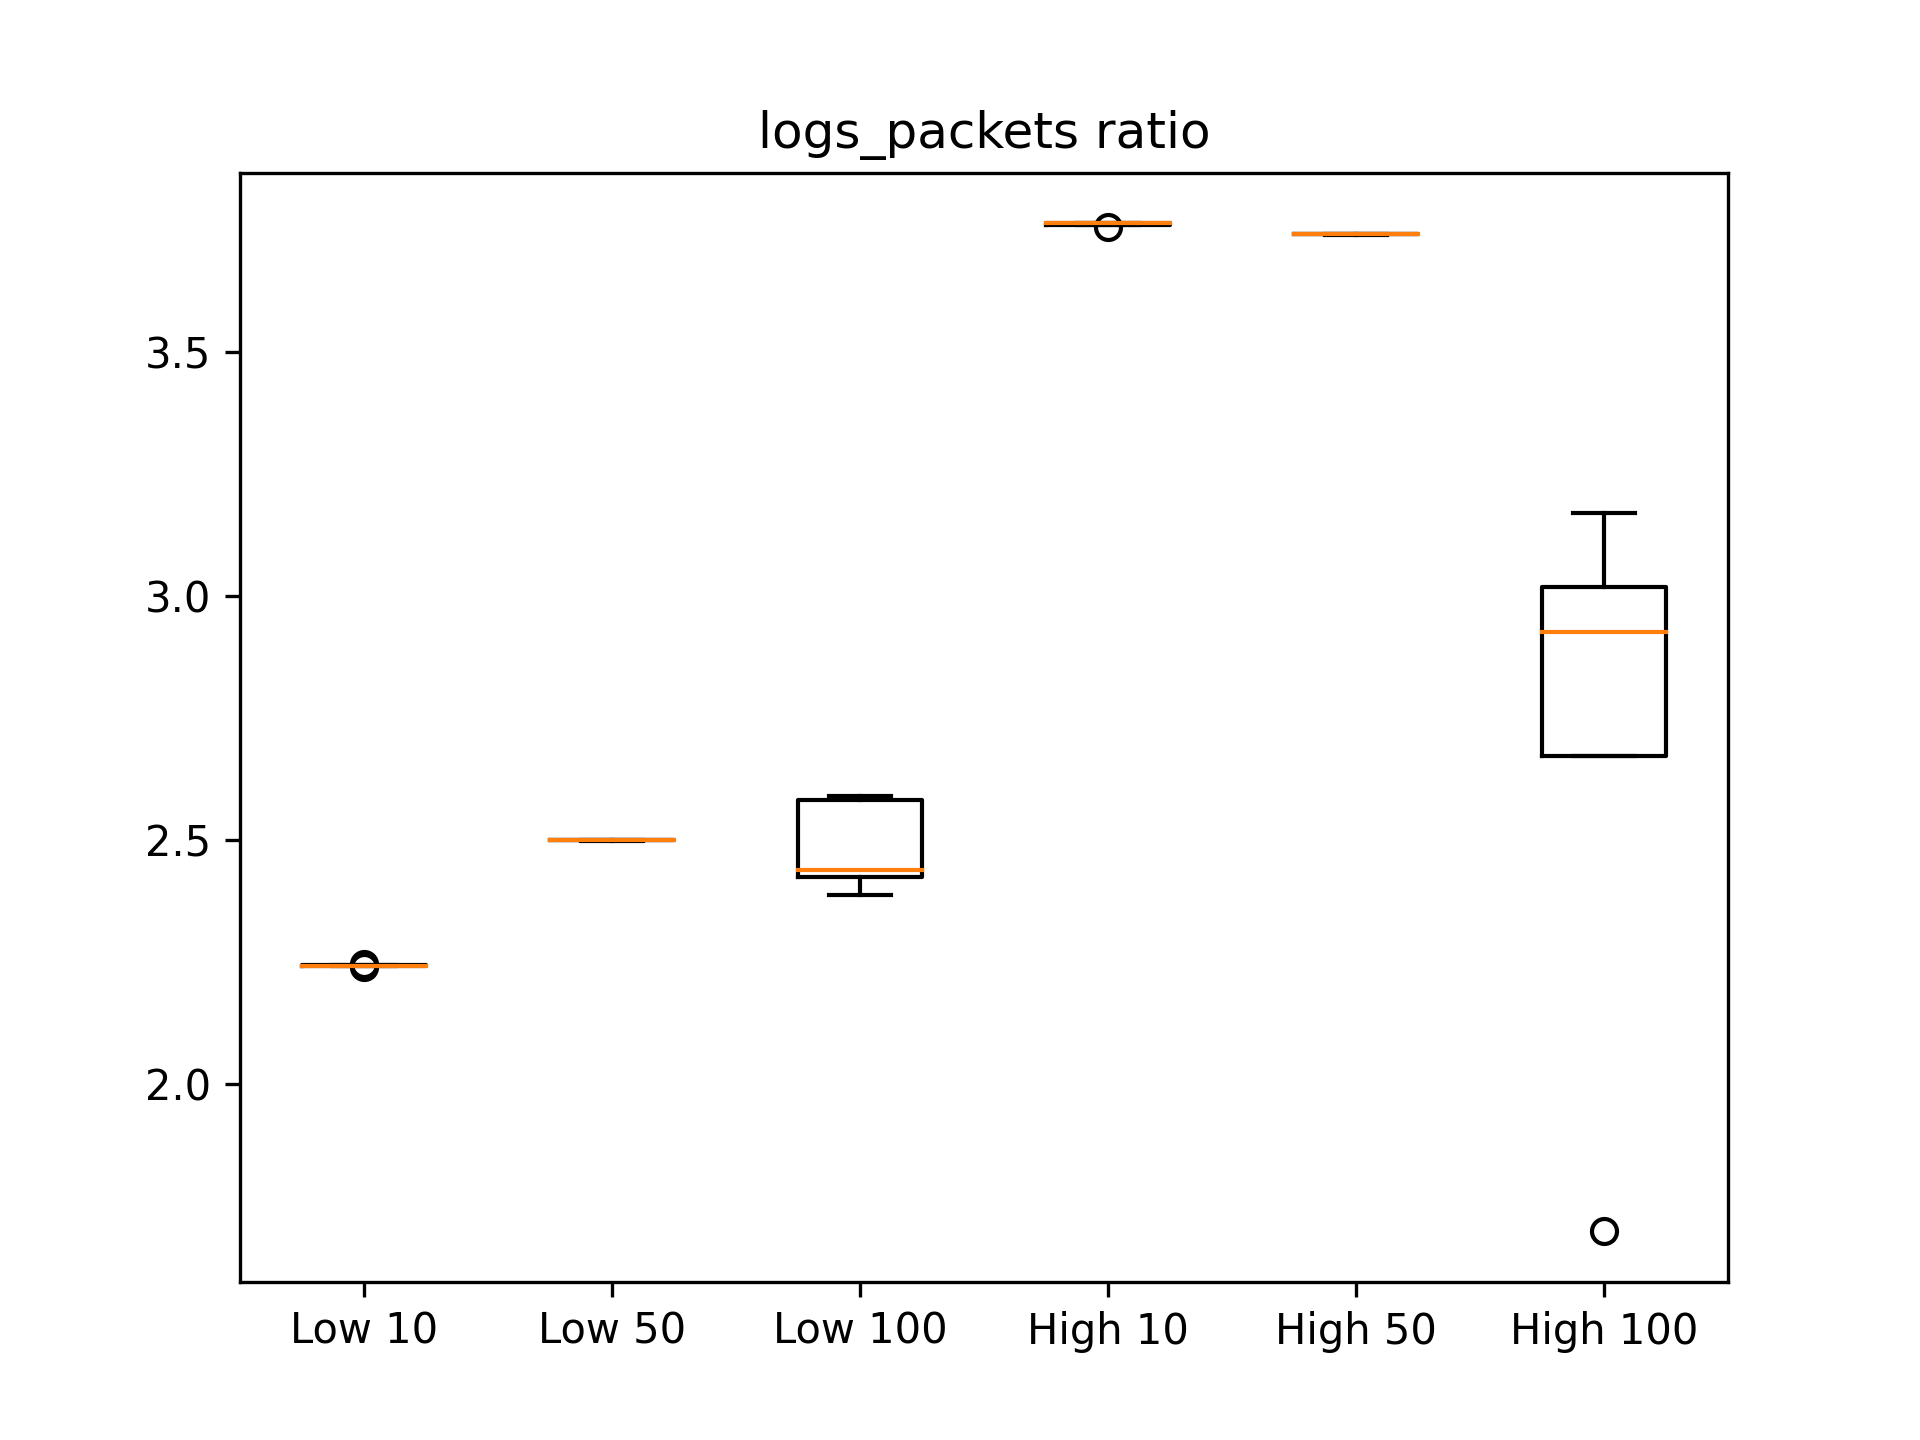
\includegraphics[width=0.7\linewidth, keepaspectratio]{graphs/logs_packets ratio.png}
    \caption{Rapporto tra pacchetti effettivamente inviati e messaggi riportati nel log}
    \label{fig:lpr}
\end{figure}

Questa metrica mette in evidenza quanti pacchetti sono \emph{inviati} (non scambiati in totale), approssimativamente, per ogni messaggio inviato.
Se il rapporto fosse minore di $1$ probabilmente saremmo in presenza di un'errore nella raccolta dei dati, a meno che il middleware non faccia ottimizzazione del recapito utilizzando una rete overlay, ma nel nostro caso non è così.

Istintivamente verrebbe da pensare che il numero di pacchetti sia influenzato dai nodi, che causano un aumento dei pacchetti per mantenere il gruppo.
Però dal grafico osserviamo che il numero di nodi influenza solo marginalmente il numero di pacchetti inviati, anzi nel caso con carico alto, la quantità di pacchetti diminuisca all'aumentare dei nodi.

Possiamo vedere che il numero di pacchetti per messaggio è influenzato principalmente dal tipo di carico. Comunque, anche sotto carico alto, sono meno di $4$ pacchetti per messaggio.

\paragraph{\lstinline{bytes per packet}}

\begin{figure}[H]
    \centering
    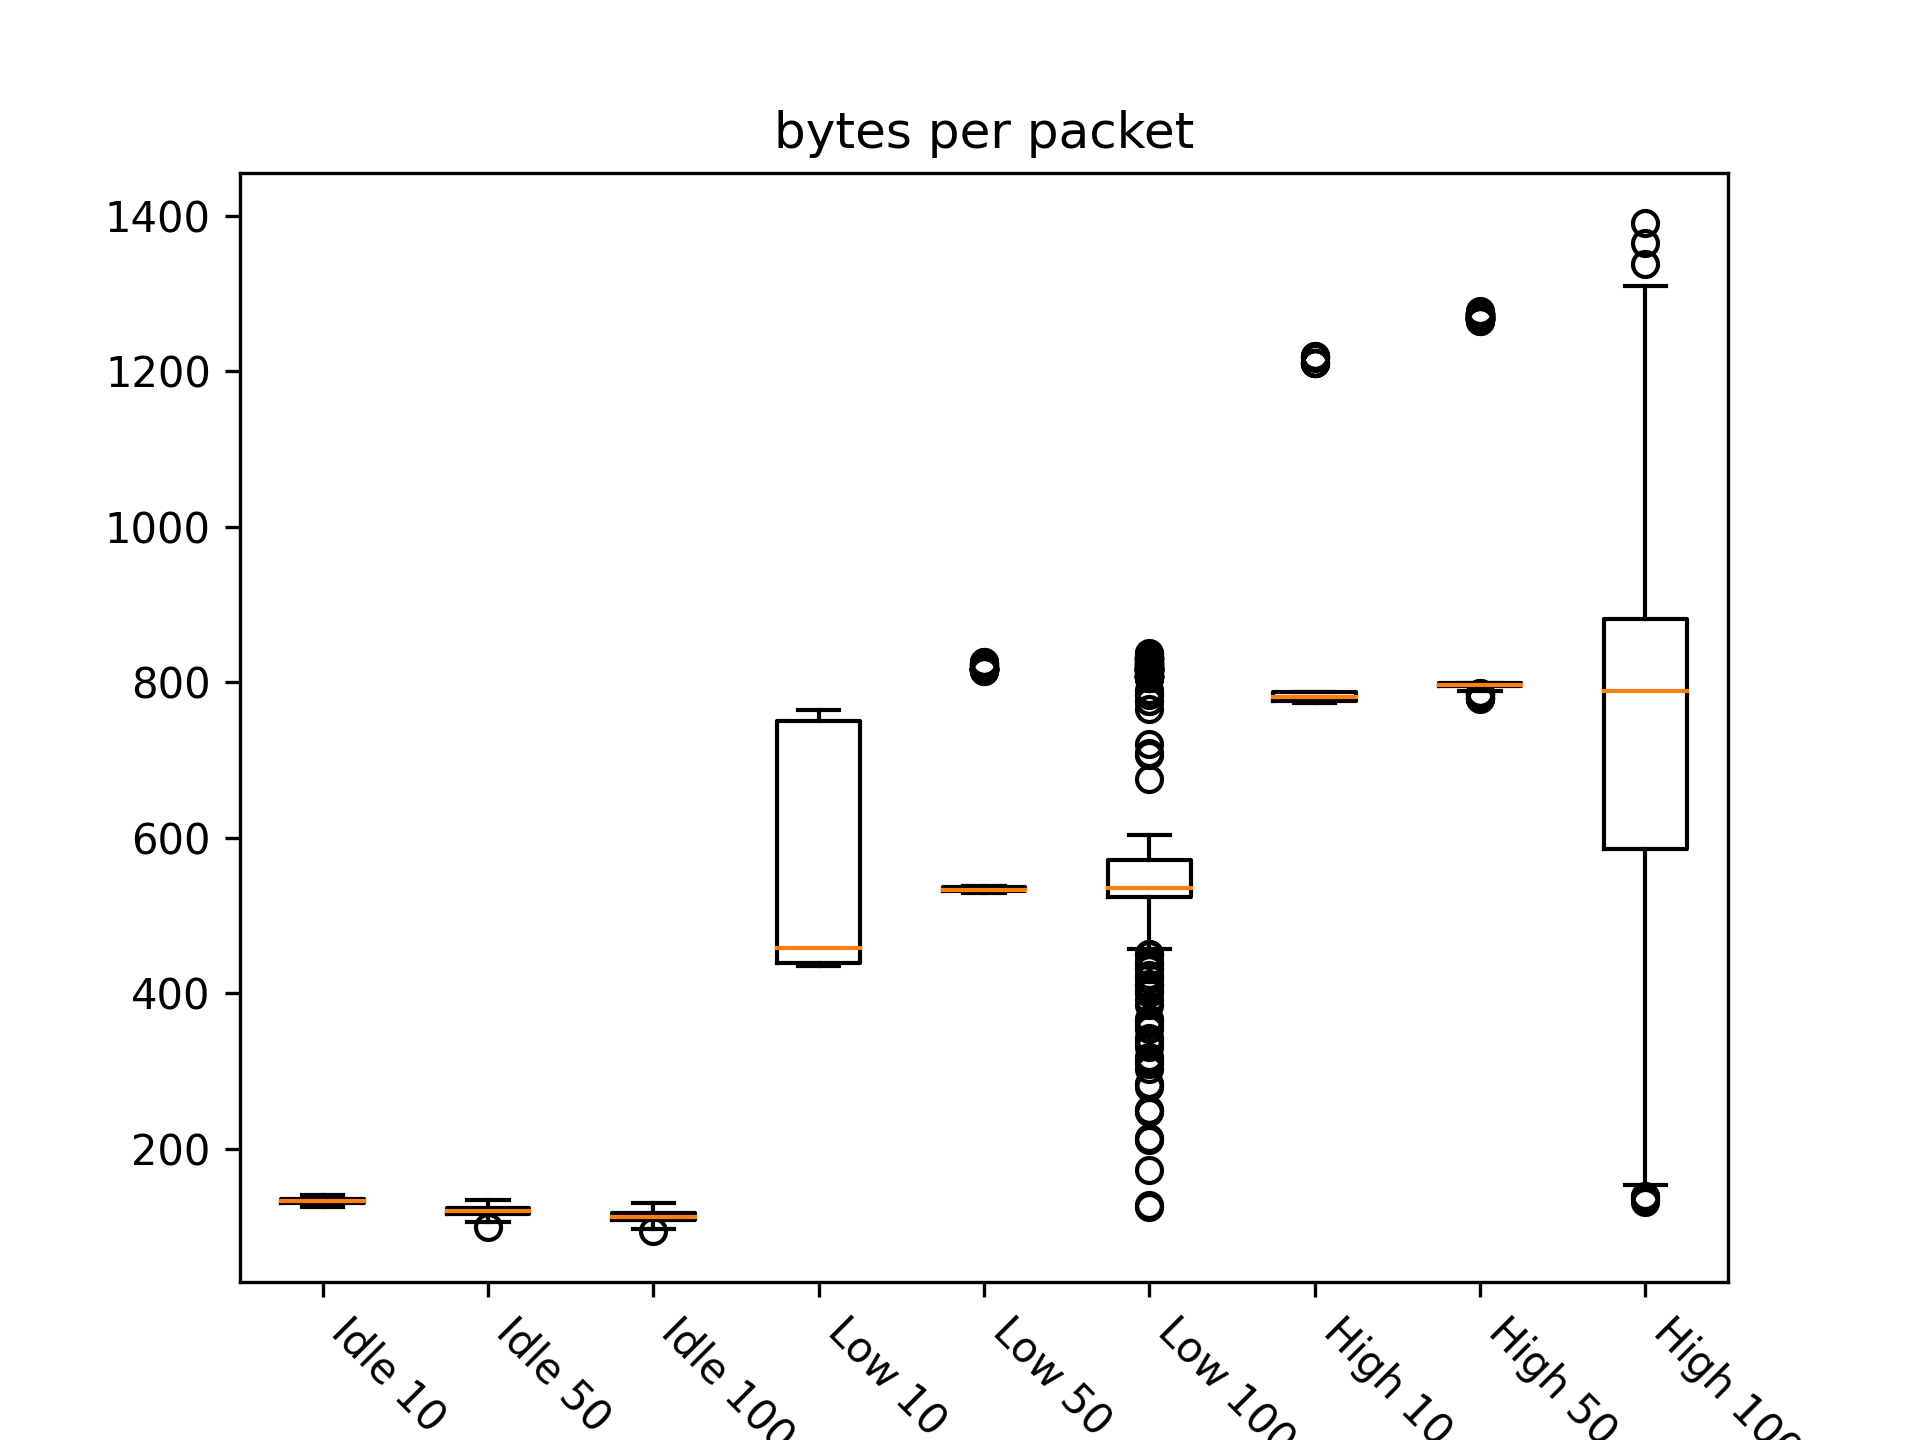
\includegraphics[width=0.7\linewidth, keepaspectratio]{graphs/bytes per packet.png}
    \caption{Dimensione in byte dei pacchetti}
    \label{fig:bp}
\end{figure}

In questo grafico è rappresentata la dimensione media dei pacchetti, ottenuta dividendo i byte per il numero di pacchetti inviati da ogni nodo per ogni computazione.

Analizzando il grafico \lstinline{total packets}~\ref{fig:tp} abbiamo notato che il numero di pacchetti inviati in idle sembrava crescere più che linearmente rispetto al numero di nodi; quando invece la quantità di dati in \lstinline{total bytes} Figure~\ref{fig:tb} sembrava quasi lineare.
Osservando questo grafico, possiamo vedere che la dimensione dei pacchetti diminuisce all'aumentare dei nodi, come ci si aspetta dai due dati precedenti.

Notiamo che come il numero di pacchetti per transizione, anche la dimensione dei pacchetti è influenzata principalmente dal tipo di carico.
Notiamo anche che nessuno dei carichi fa raggiungere consistentemente la \lstinline{MTU} (che è di $\qty{1500}{\byte}$).

Nonostante fosse così anche nelle altre metriche, in questa risulta molto evidente che all'aumentare dei nodi, i risultati diventano sempre più imprecisi.
Alcuni nodi ricevono più o meno traffico. Anche se i messaggi sono in broadcast e dovrebbero essere distribuite tra tutti i nodi.
Probabilmente si tratta di un'effetto del gossiping probabilistico in una rete molto grande.

\section{Conclusioni e proposte di miglioramento}

Dopo aver analizzato questi risultati, possiamo concludere che GoAbU non riesce a scalare come sperato. La libreria riesce a mantenere un costo per regola non troppo alto quando si arriva a grandi quantità di regole esterne.Ma il traffico complessivo rimane troppo alto (vedi Figure~\ref{fig:tb} e Figure~\ref{fig:tp}).

Il middleware riesce ridurre ulteriormente il traffico grazie ad un qualche meccanismo di compressione (vedi Figure~\ref{fig:lbr}), questo permette a GoAbU di scalare leggermente di più. Comunque, una codifica più efficiente dei messaggi permetterebbe di ridurre l'affidamento che facciamo sulla compressione. Ma per permettere veramente a GoAbU di scalare su reti più grandi, la soluzione non è ridurre la dimensione dei messaggi.

Possiamo imputare il problema al modello di broadcast implementato, in cui ogni nodo contatta ogni altro nodo in unicast, seguendo il modello ``reliable/atomic broadcast''~\cite{joseph1989reliable}.
Potremmo migliorare le prestazioni utilizzando anche a più basso livello la comunicazione broadcast, invece che simularlo in una rete unicast. Però questo richiede di modificare la semantica del linguaggio per quanto riguarda la decisione della consegna delle regole.
Inoltre, in questo modo, non solo tutti i segmenti della rete (inclusi quelli che non usano GoAbU) riceverebbero i pacchetti di GoAbU, ma bisognerebbe gestire in modo speciale i nodi che non si trovano nella stessa LAN.

Sfruttando le assunzioni già esistenti sulla rete, in particolare completezza della rete e fair loss, si potrebbe scegliere di limitare ad numero di nodi $k$ a cui viene inoltrato il messaggio di broadcast e fare maggiore affidamento sul gossiping.
Ovviamente è necessario scegliere opportunamente questo $k$ in modo che il broadcast resti affidabile, e magari si può rendere configurabile per adattarsi alle necessità di sistemi specifici.\\
In questo modo si eviterebbe di modificare troppo il modello, pur riducendo anche di molto la message complexity del sistema.

Si può ottenere un risultato migliore utilizzando algoritmi di broadcast efficiente, basati magari sull'utilizzo di una rete overlay non completa e sull'inoltro dei messaggi.
Un metodo del genere può ridurre di molto il traffico, ma ad un costo, sia di latenza, che soprattutto computazionale. E ricordiamo che per l'utilizzo in campo IoT è necessario trovare un algoritmo che possa essere utilizzato anche da dispositivi molto piccoli.

Ad ogni modo, il paradigma del calcolo AbU ha delle grandi potenzialità, grazie alla sua semplicità di programmazione. Ed è particolarmente adatto alla coordinazione di grandi sistemi, fornendo un modo semplice di diffondere informazioni.
Anche se GoAbU non è ancora adatto a scalare, è solo la prima implementazione, e ci sono ancora molte opzioni per migliorare.




%% Fine dei capitoli normali, inizio dei capitoli-appendice (opzionali)
\appendix

%\part{Appendici}

\chapter{Altri grafici}\label{appendix:grafici}

\begin{figure}[H]
    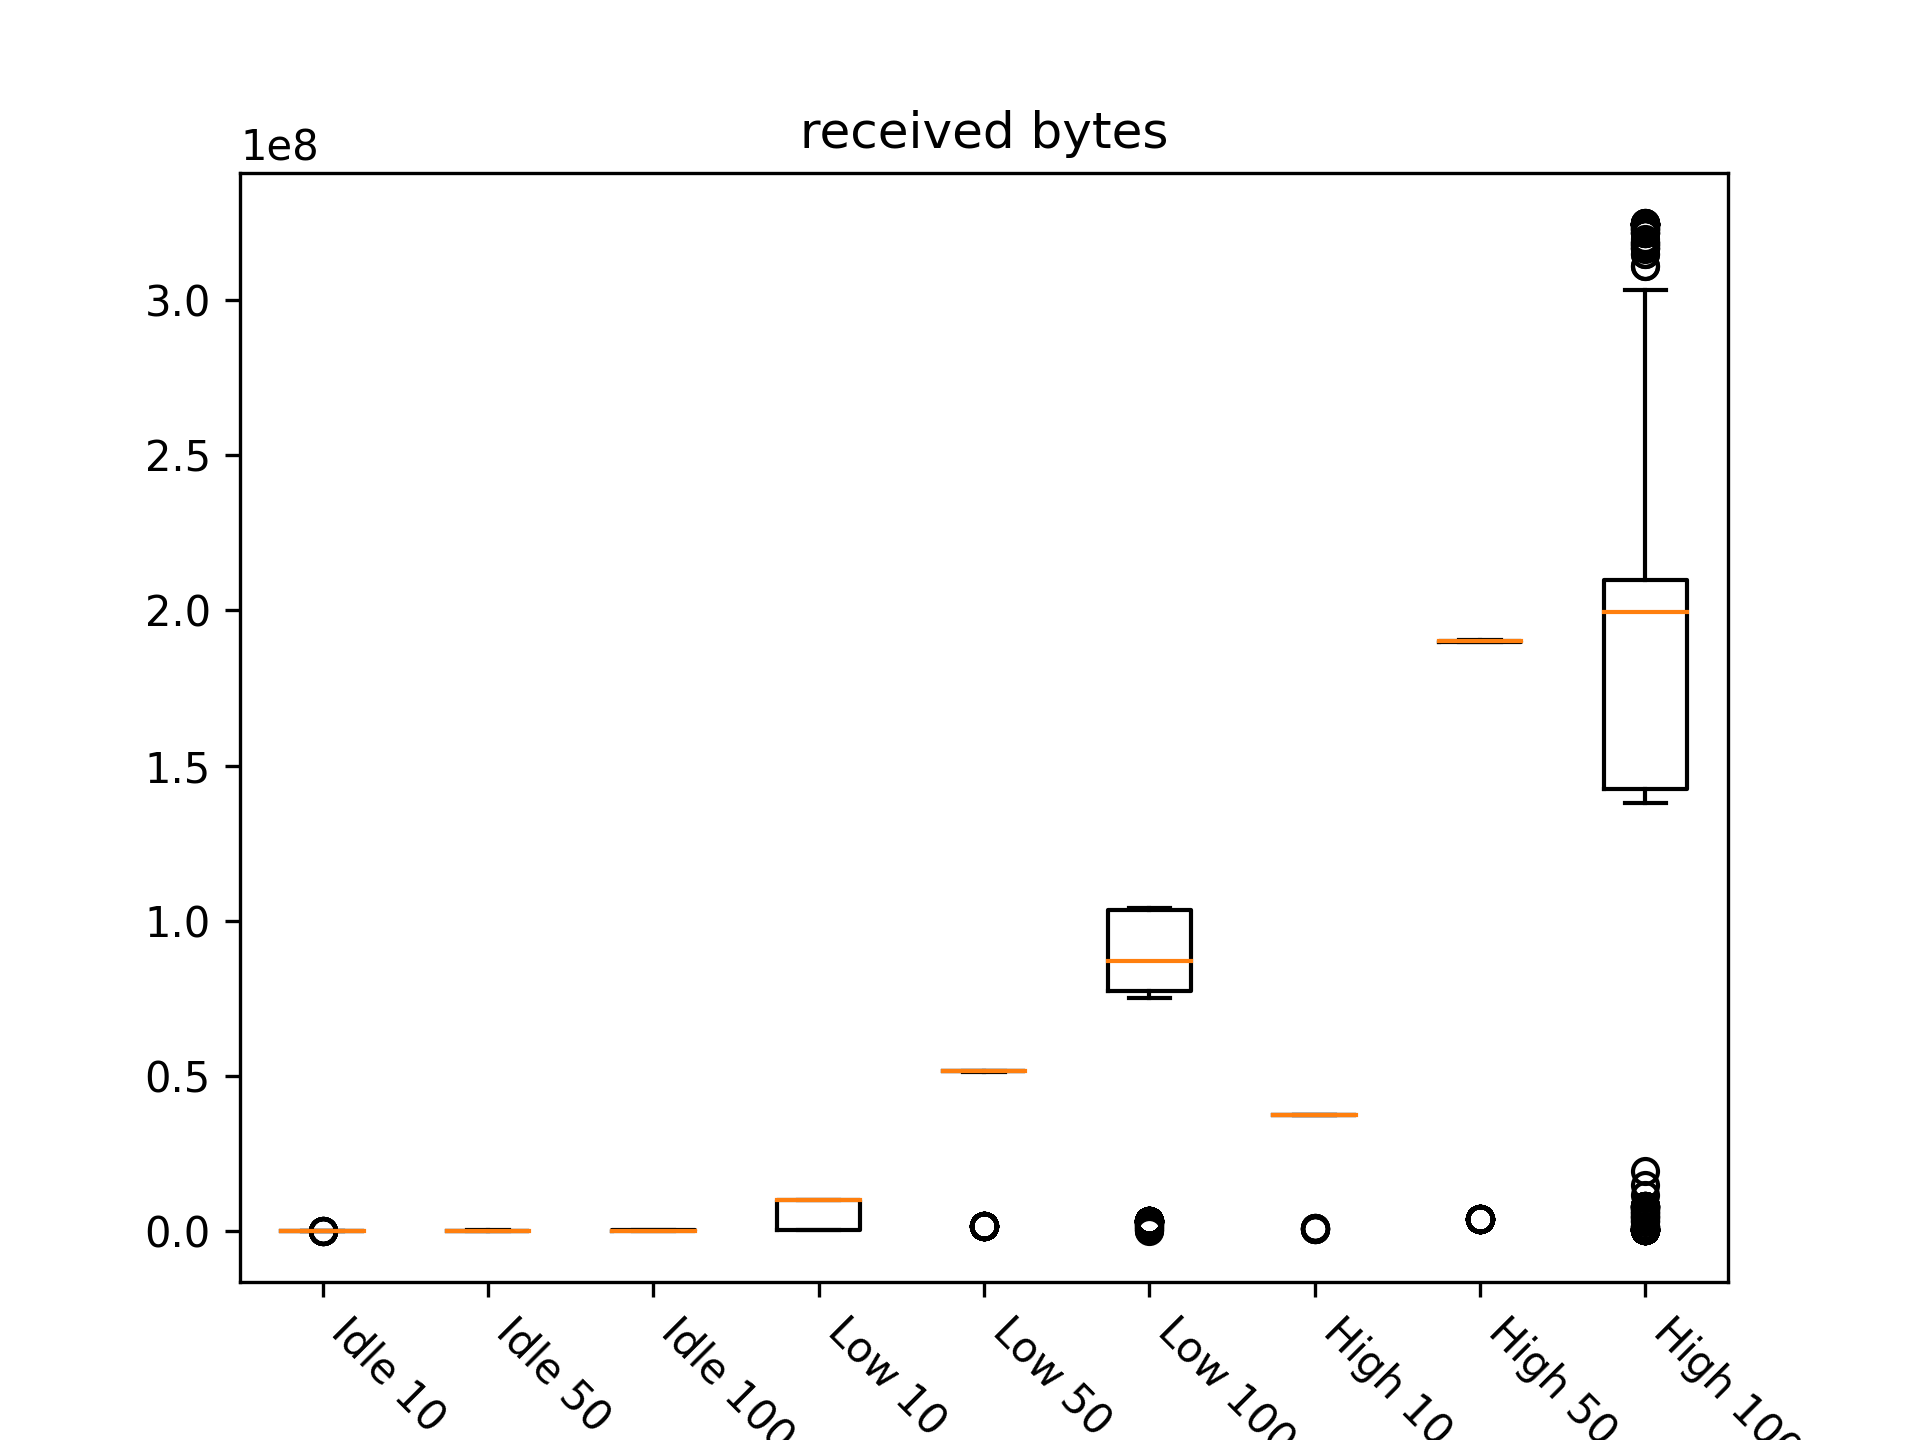
\includegraphics[width=\linewidth, height=0.4\textheight, keepaspectratio]{graphs/received bytes.png}
    \caption{Indica il numero totale di byte ricevuti da un agente in un test}
    \label{fig:rb}
\end{figure}

\begin{figure}[H]
    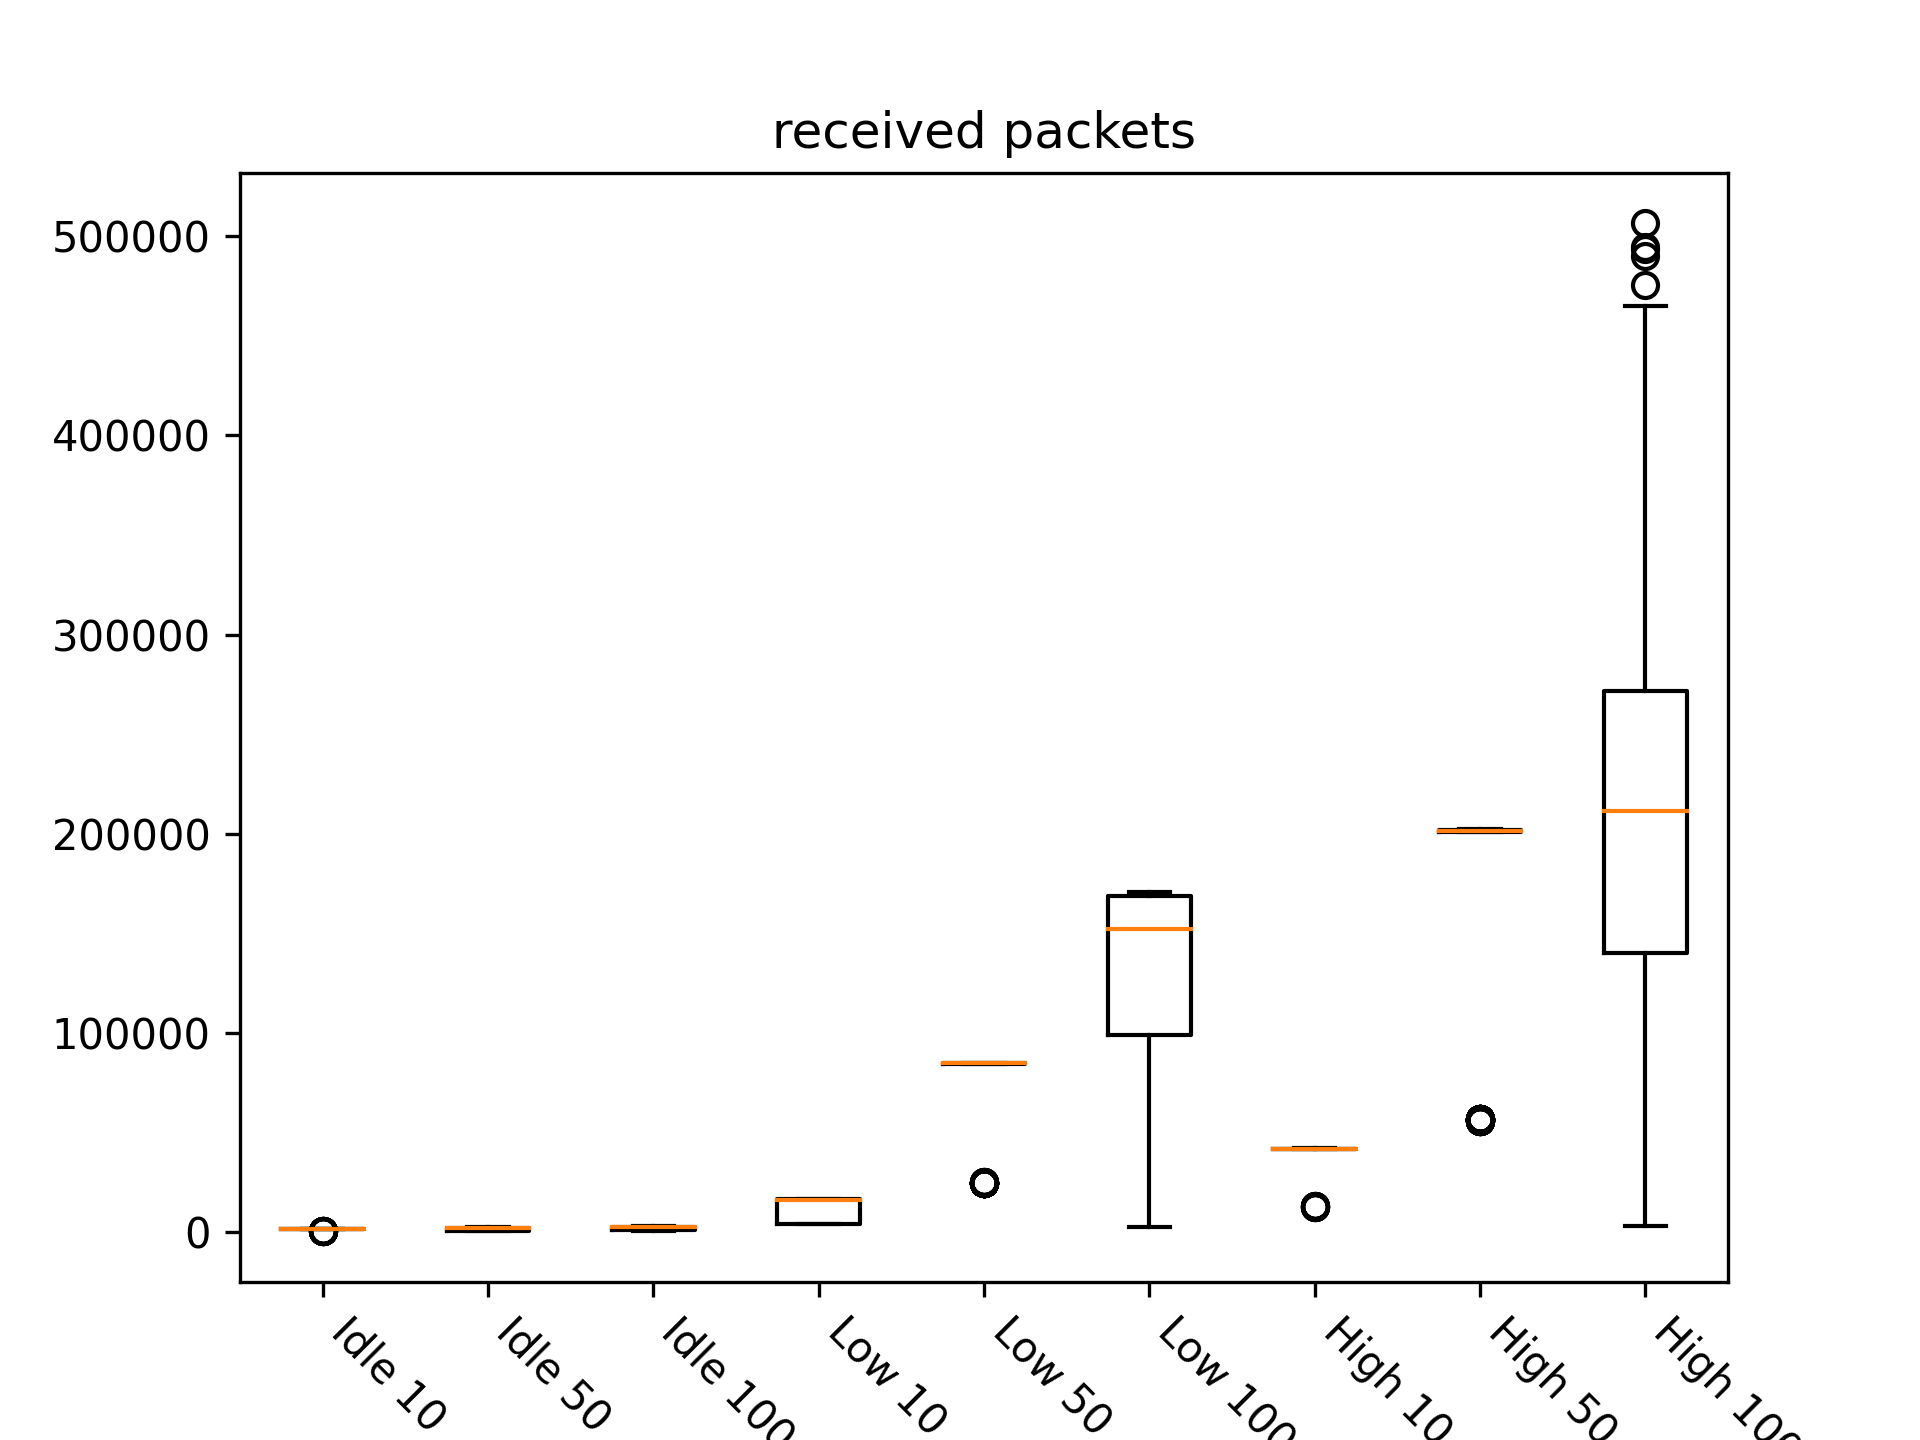
\includegraphics[width=\linewidth, height=0.4\textheight, keepaspectratio]{graphs/received packets.png}
    \caption{Indica il numero totale di pacchetti ricevuti da un agente in un test}
    \label{fig:rp}
\end{figure}

\begin{figure}[H]
    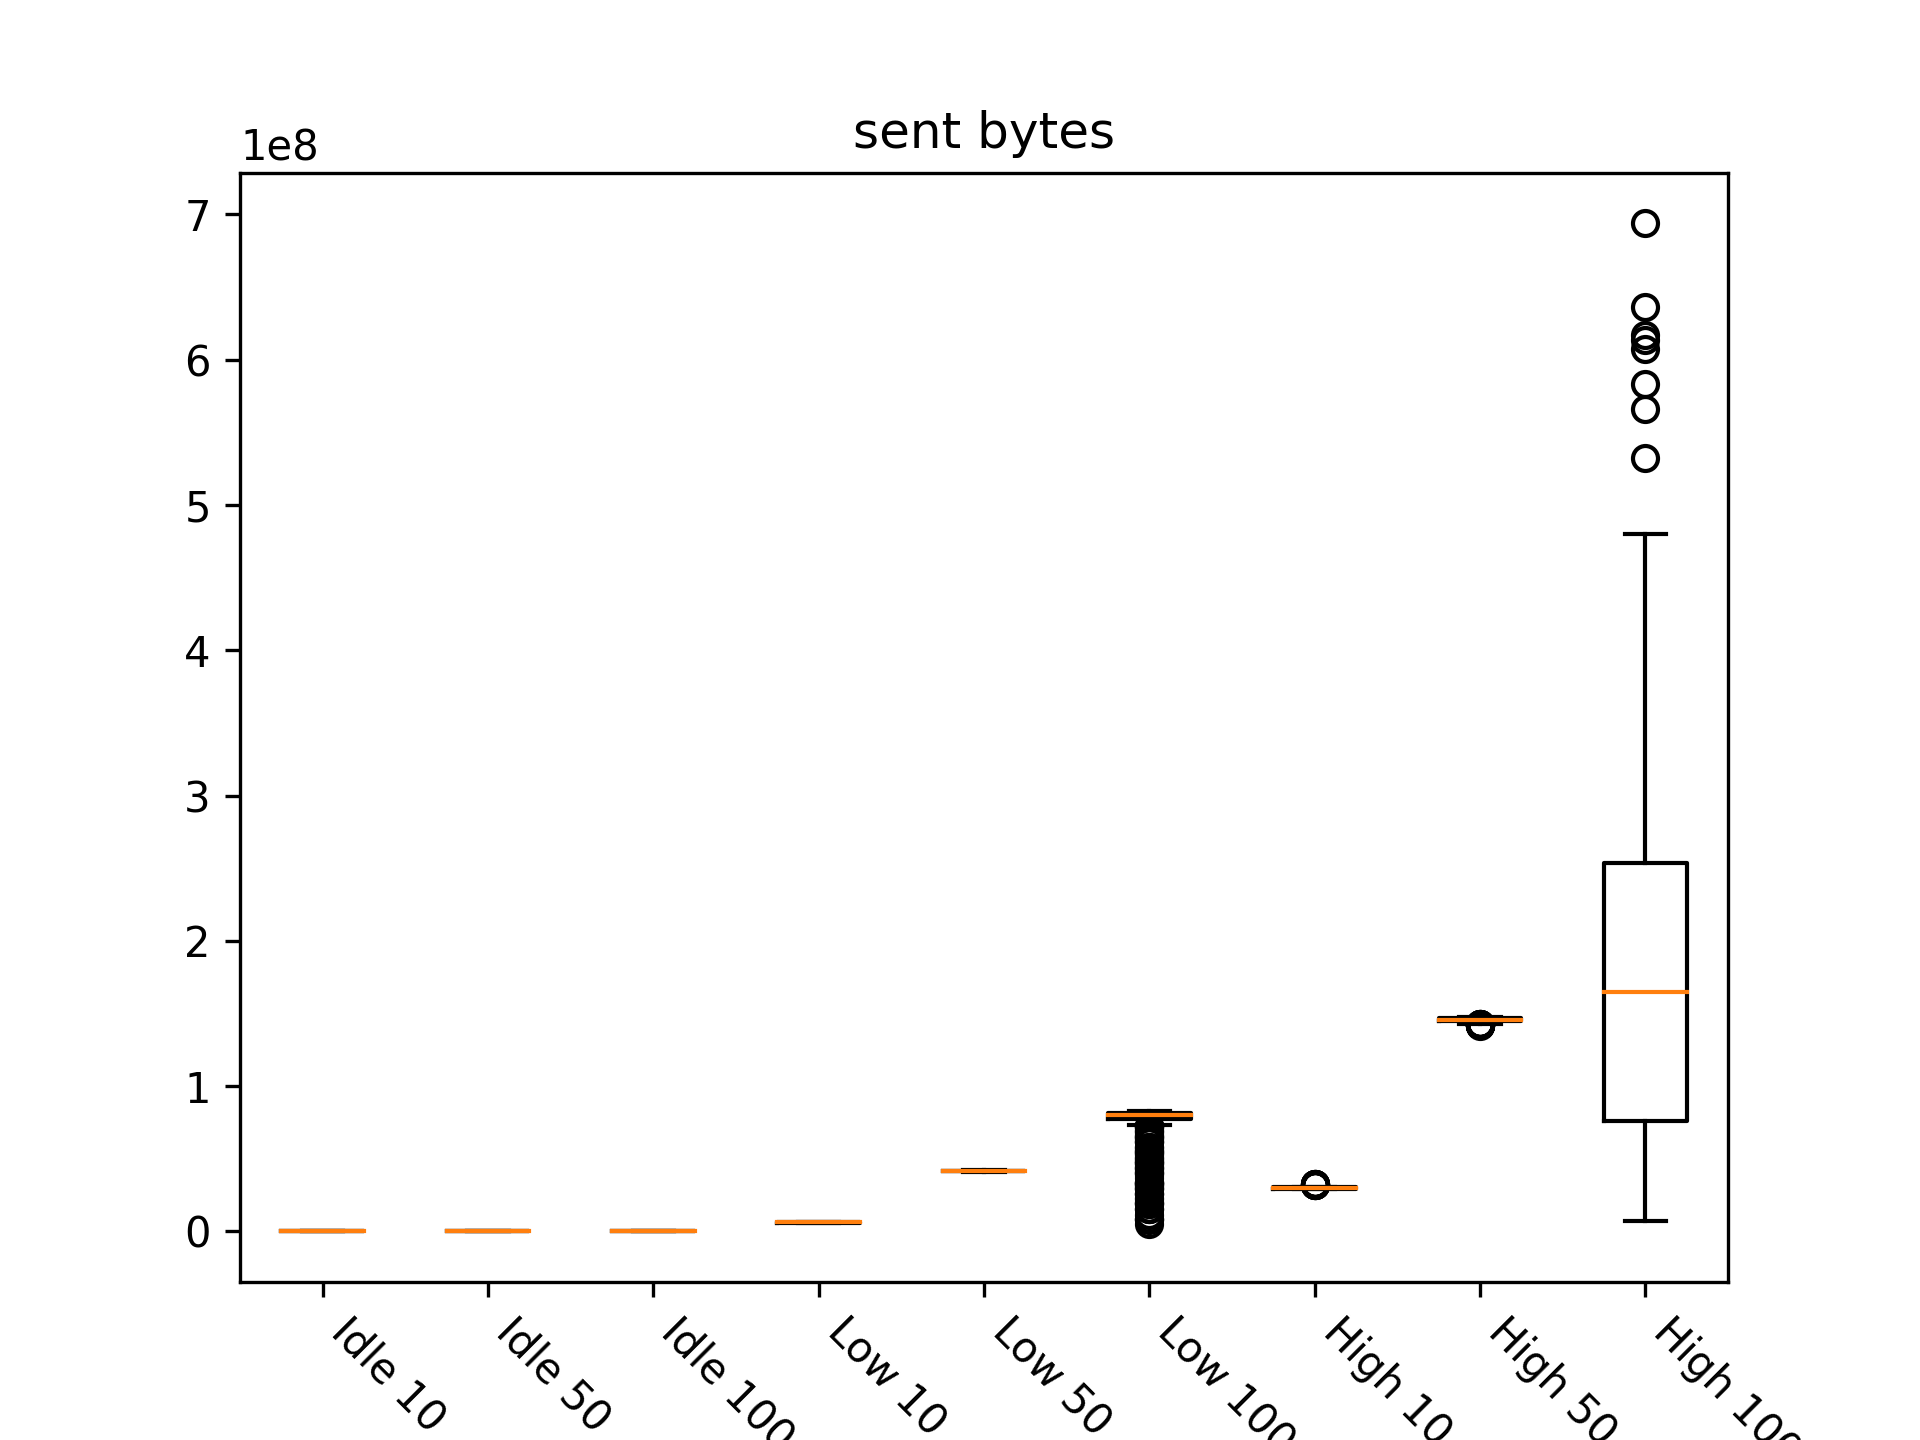
\includegraphics[width=\linewidth, height=0.4\textheight, keepaspectratio]{graphs/sent bytes.png}
    \caption{Indica il numero totale di byte inviati da un agente in un test}
    \label{fig:sb}
\end{figure}

\begin{figure}[H]
    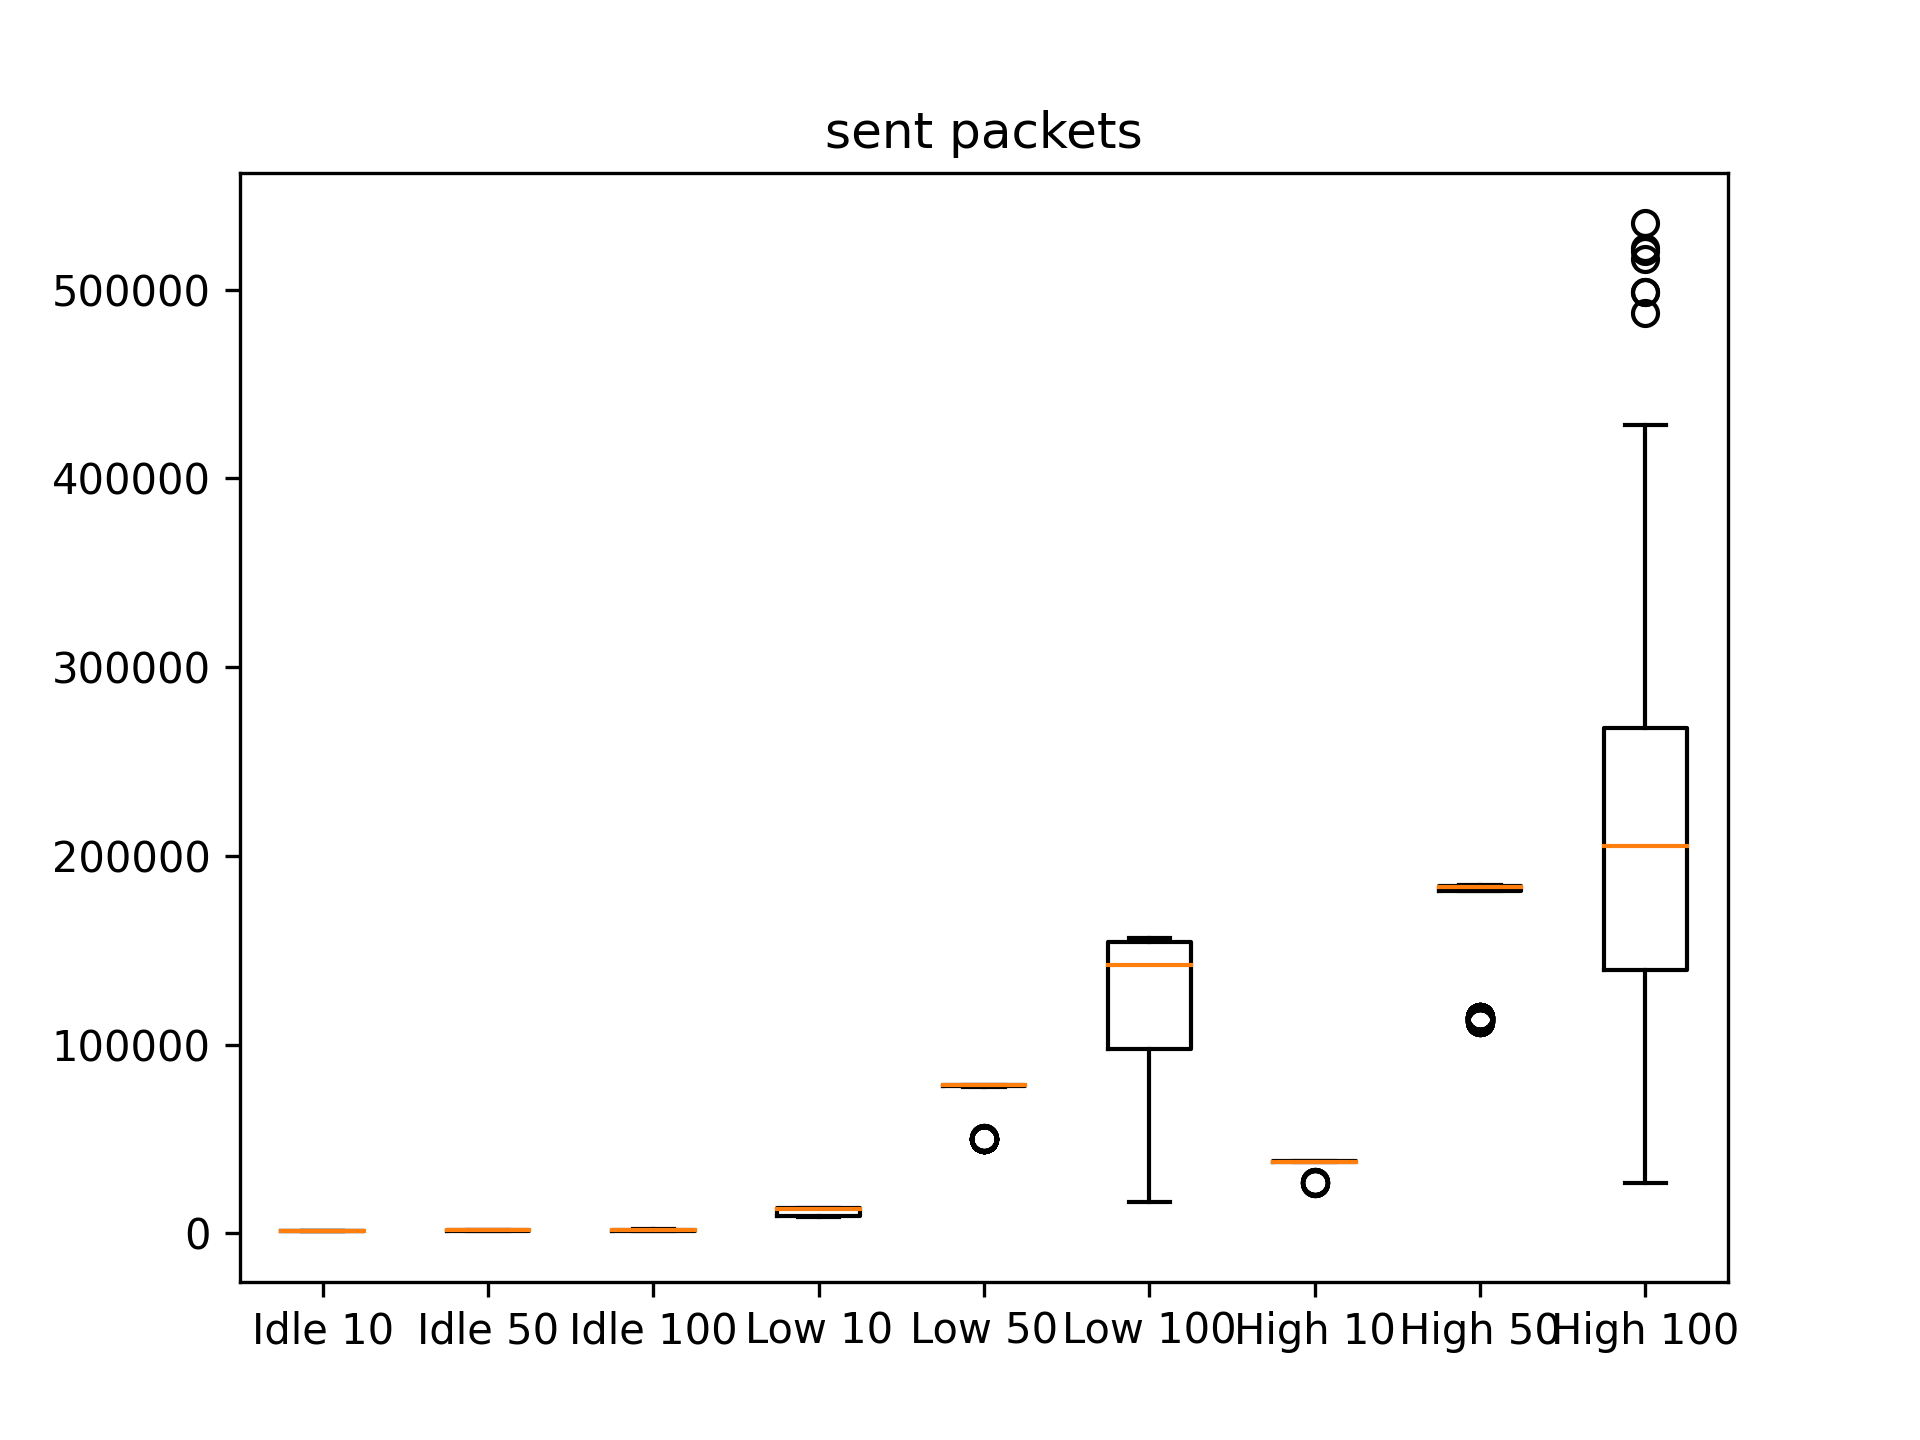
\includegraphics[width=\linewidth, height=0.4\textheight, keepaspectratio]{graphs/sent packets.png}
    \caption{Indica il numero totale di pacchetti inviati da un agente in un test}
    \label{fig:sp}
\end{figure}

\begin{figure}[H]
    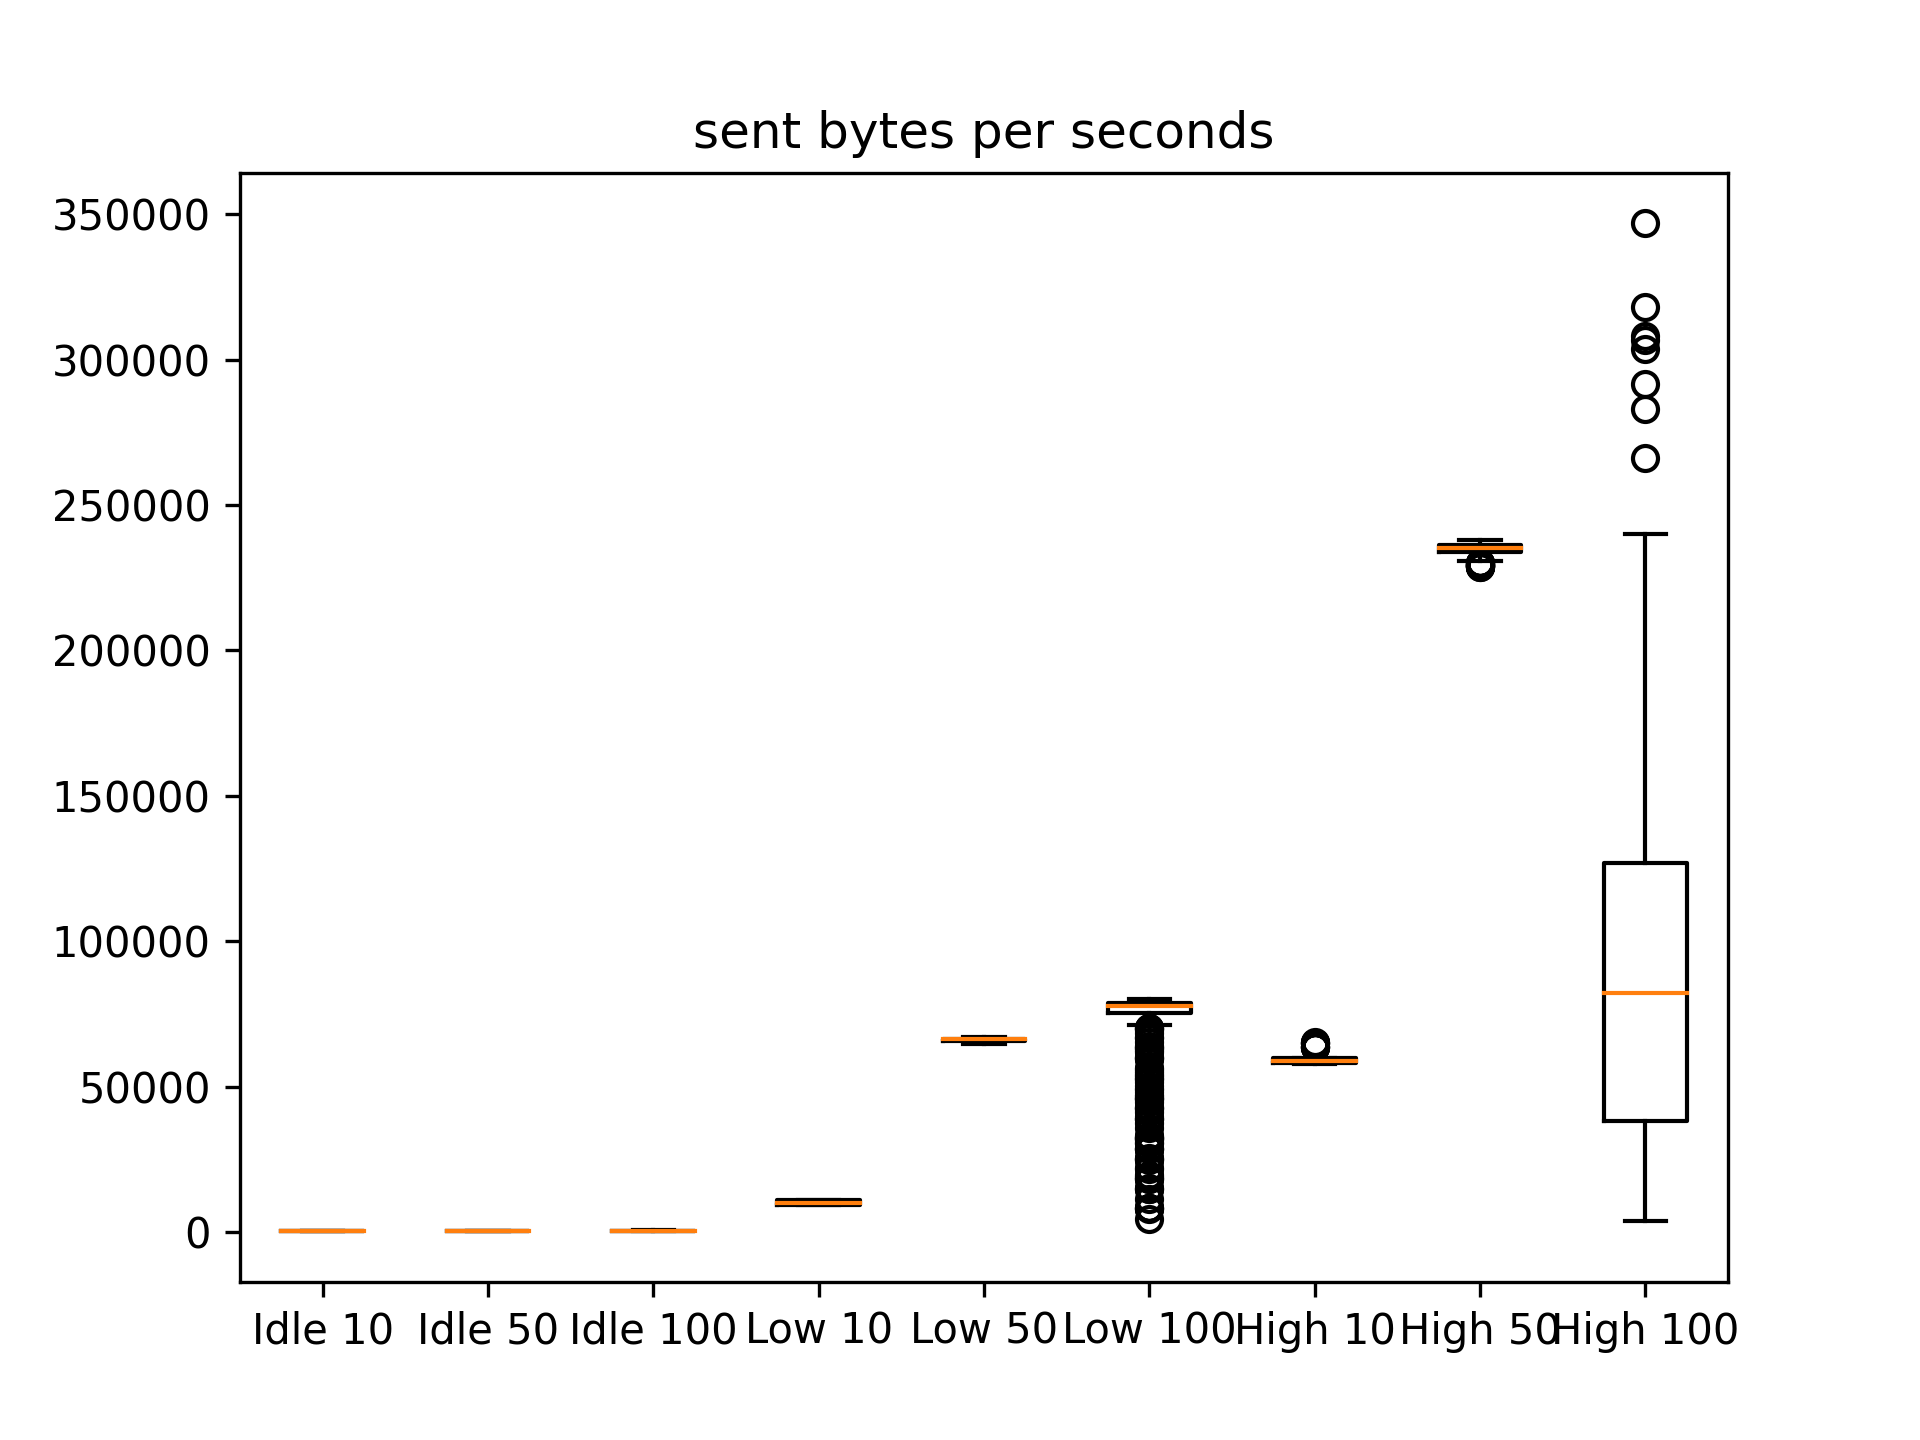
\includegraphics[width=\linewidth, height=0.4\textheight, keepaspectratio]{graphs/sent bytes per seconds.png}
    \caption{Come sopra, ma diviso per la durata del test}
    \label{fig:sbps}
\end{figure}

\begin{figure}[H]
    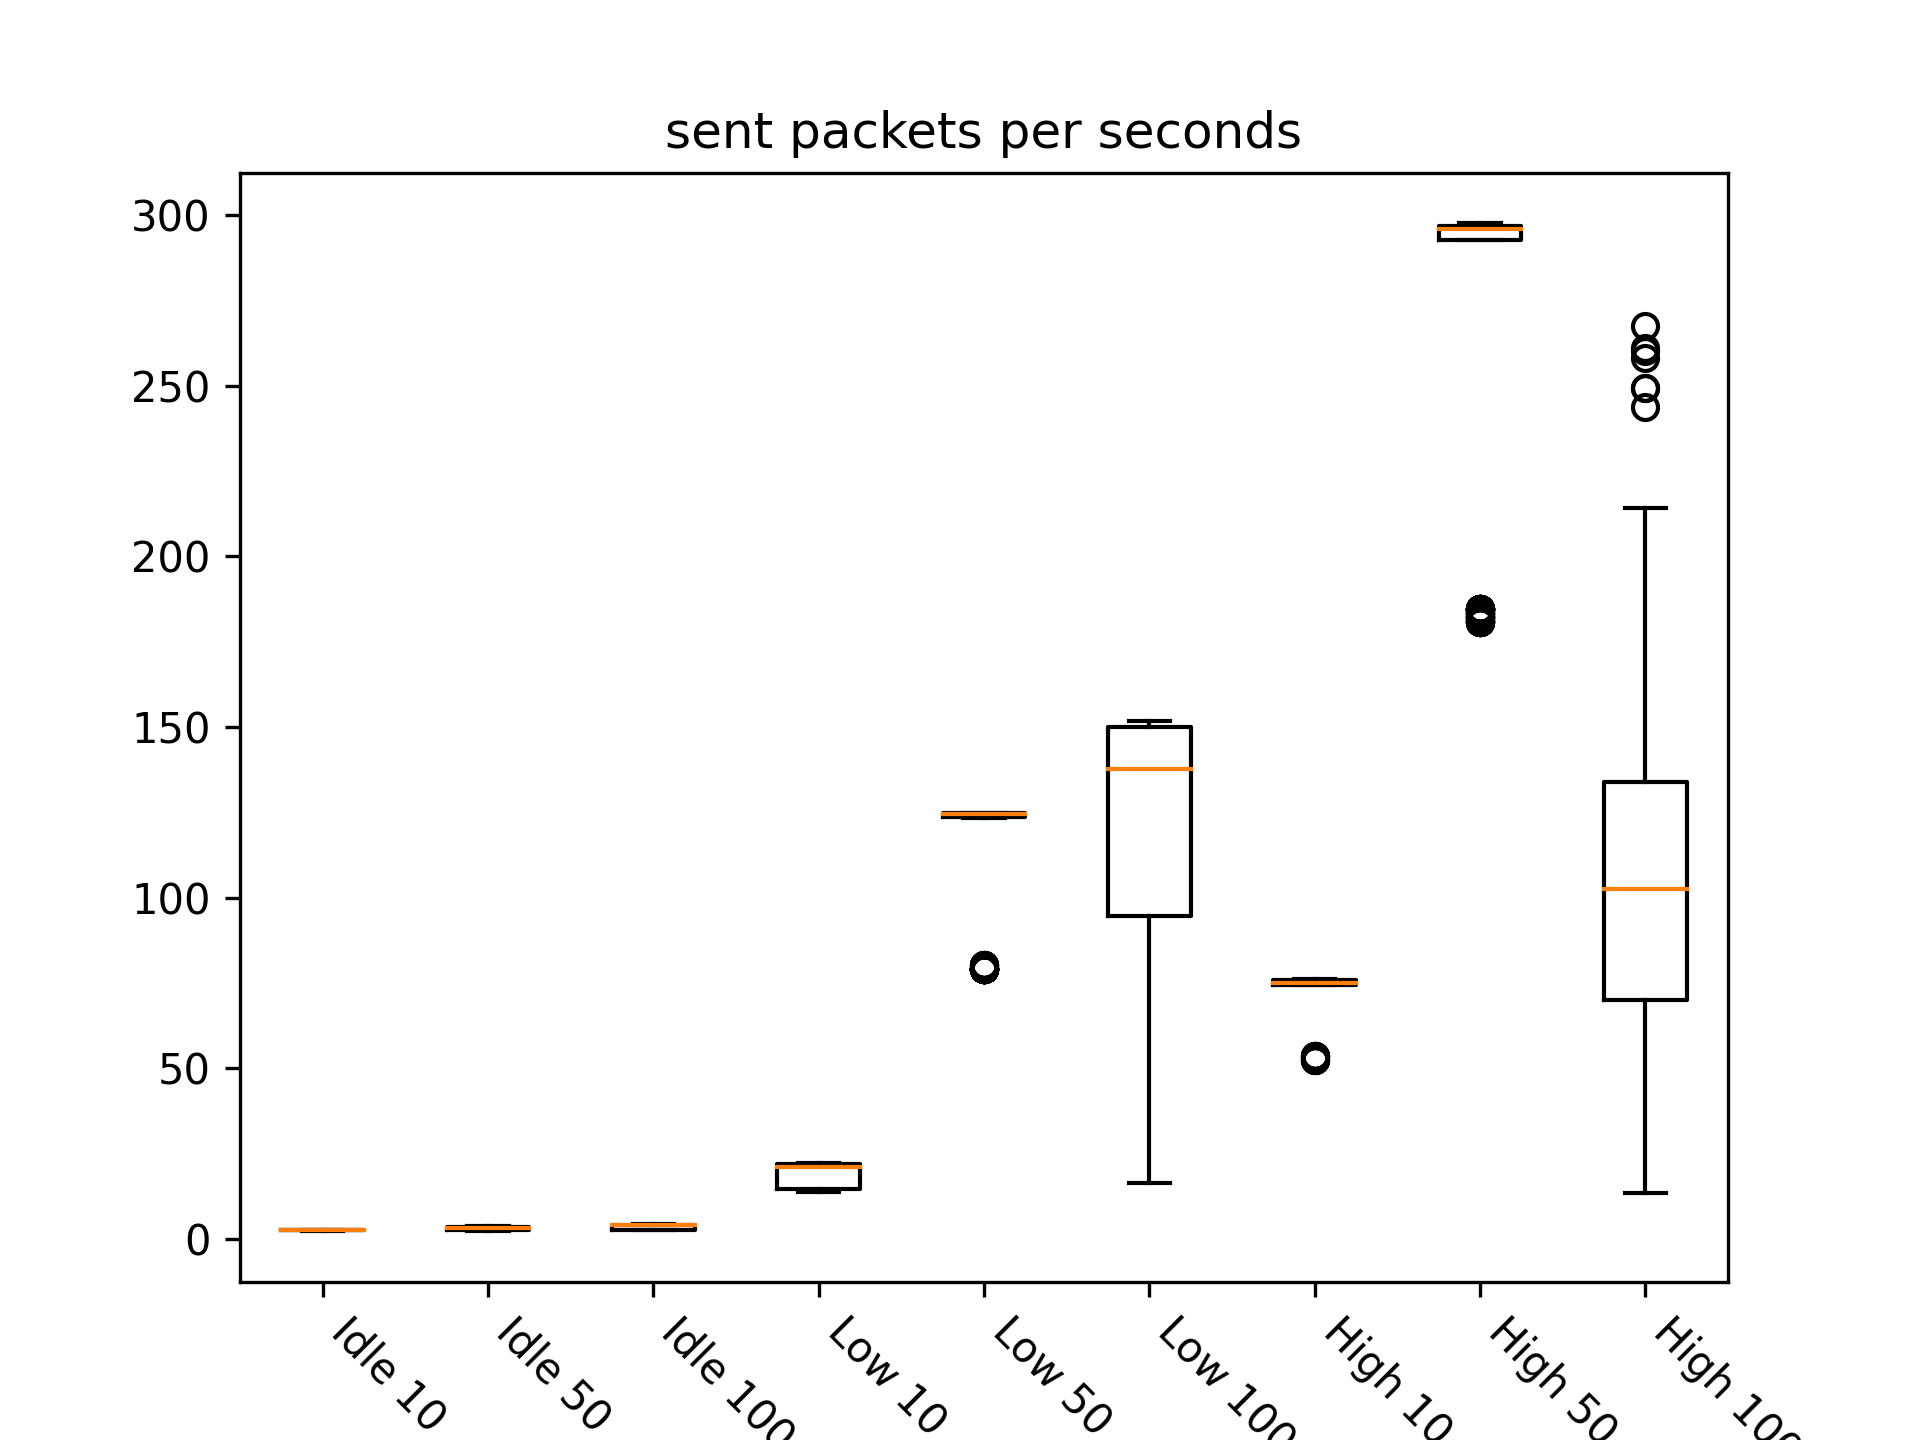
\includegraphics[width=\linewidth, height=0.4\textheight, keepaspectratio]{graphs/sent packets per seconds.png}
    \caption{Come sopra, ma diviso per la durata del test}
    \label{fig:spps}
\end{figure}

\begin{figure}[H]
    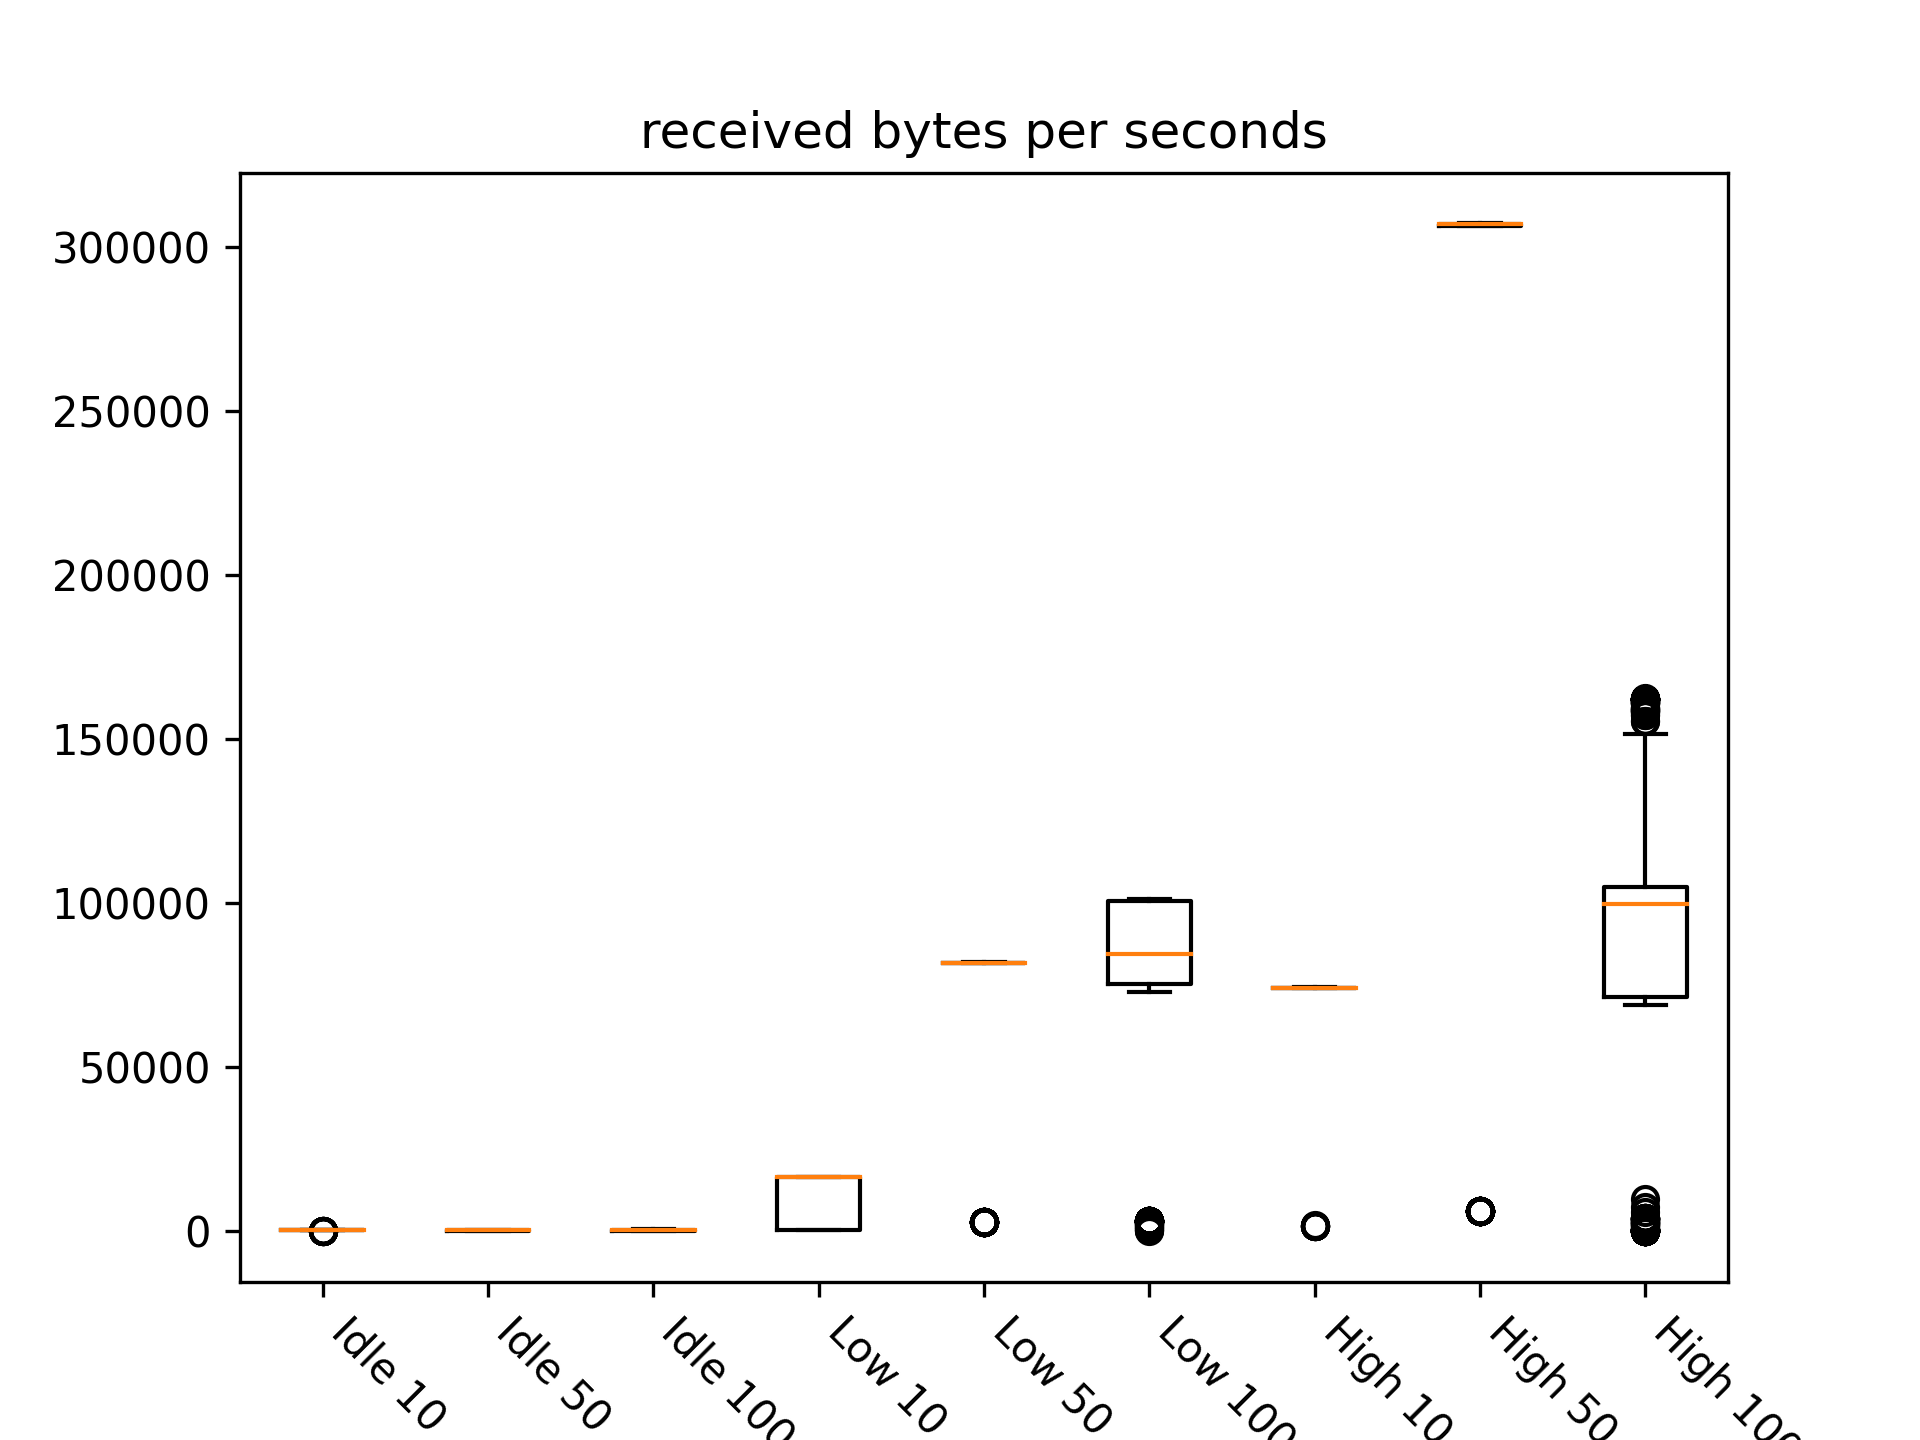
\includegraphics[width=\linewidth, height=0.4\textheight, keepaspectratio]{graphs/received bytes per seconds.png}
    \caption{Come sopra, ma diviso per la durata del test}
    \label{fig:rbps}
\end{figure}

\begin{figure}[H]
    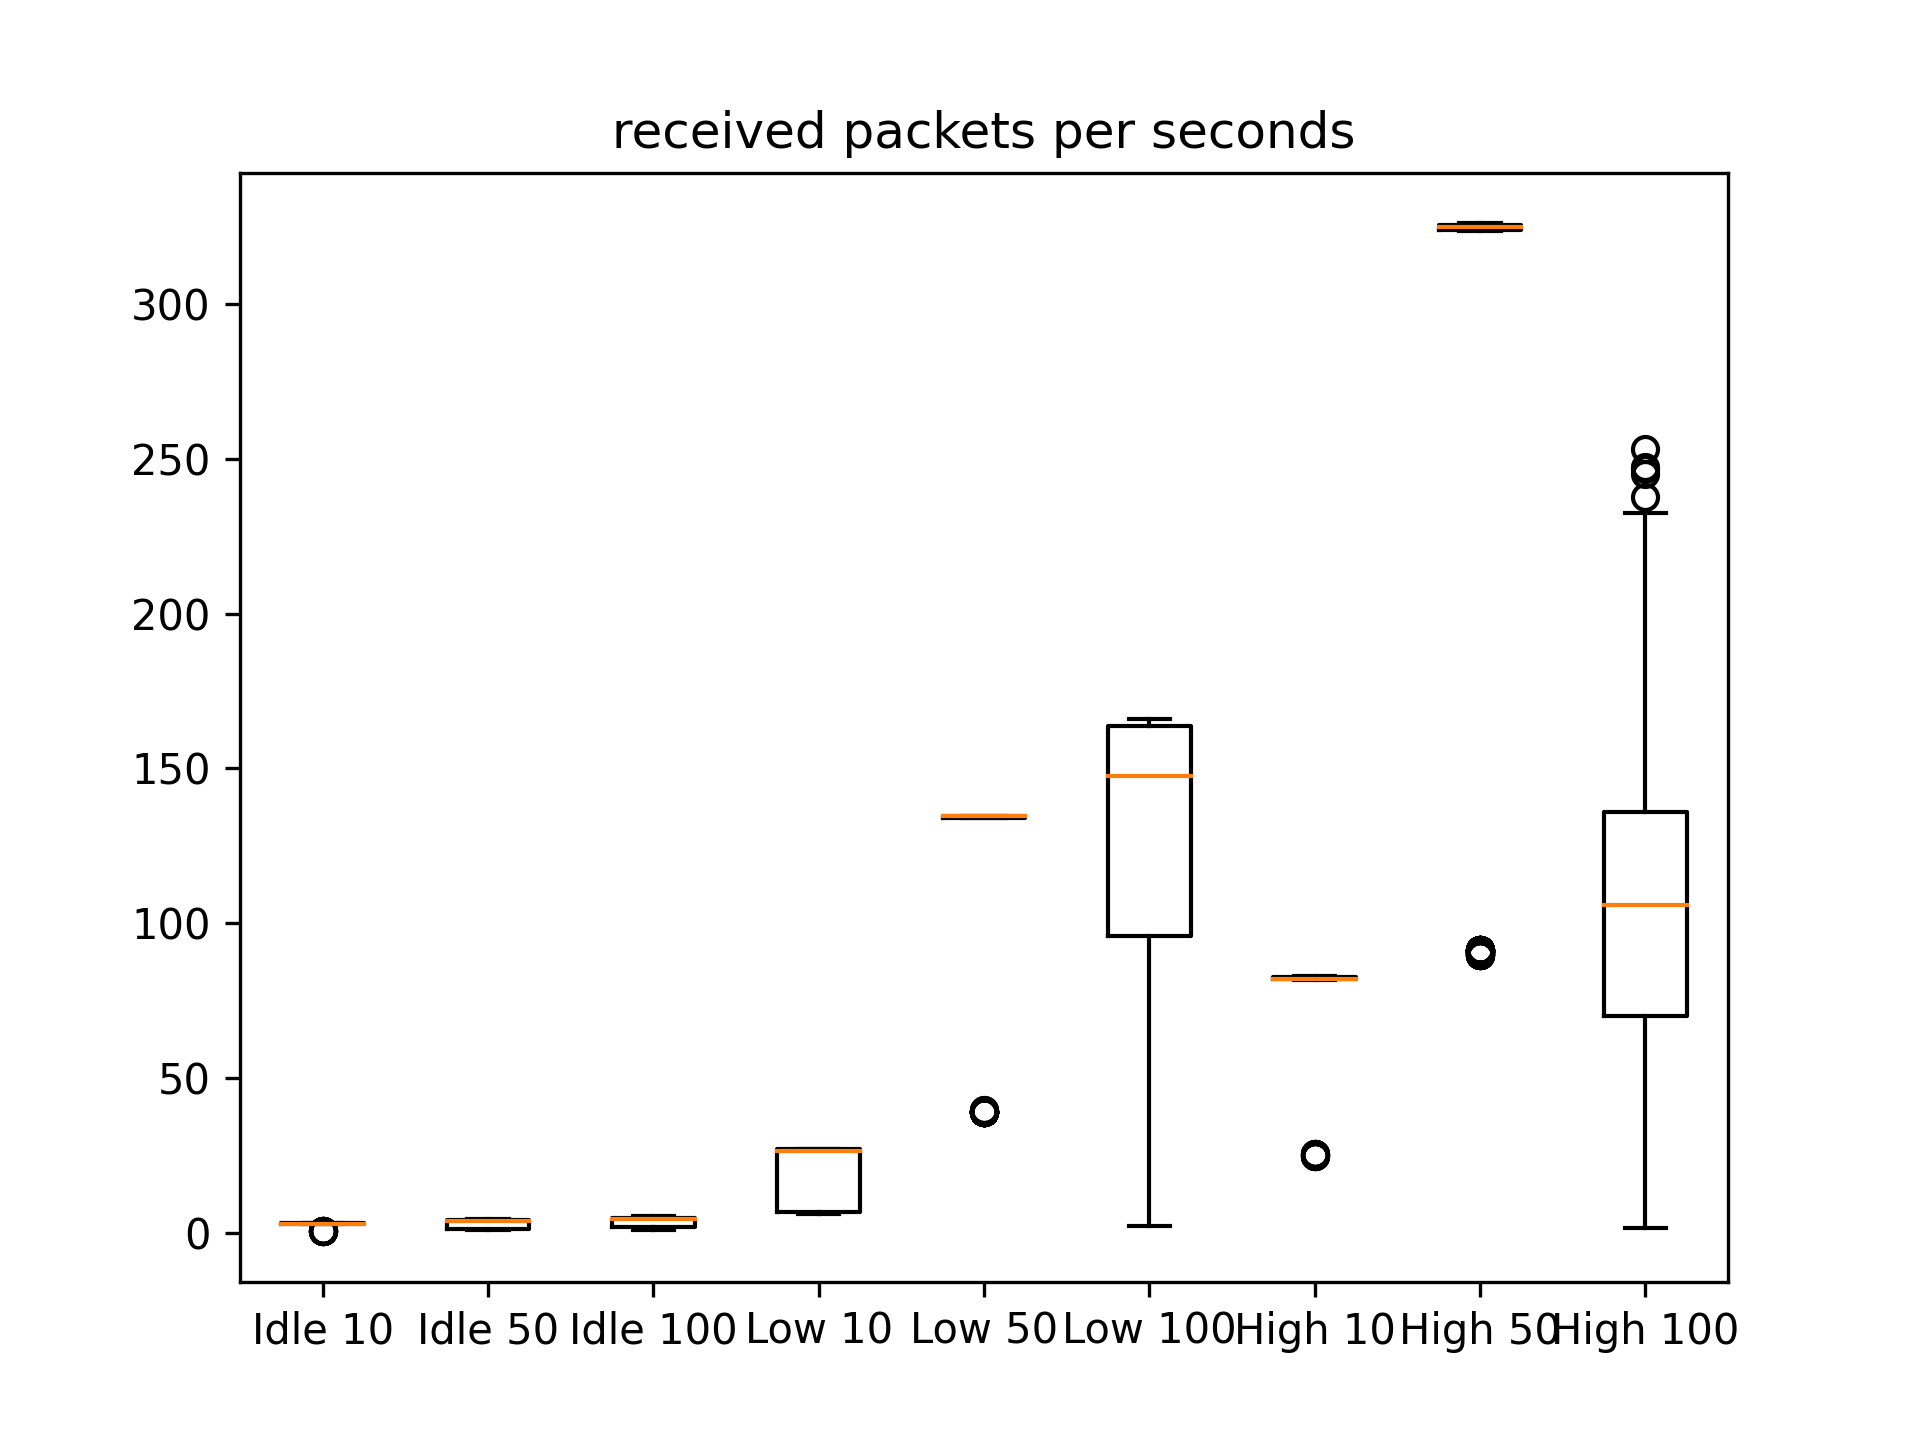
\includegraphics[width=\linewidth, height=0.4\textheight, keepaspectratio]{graphs/received packets per seconds.png}
    \caption{Come sopra, ma diviso per la durata del test}
    \label{fig:rpps}
\end{figure}

\begin{figure}[H]
    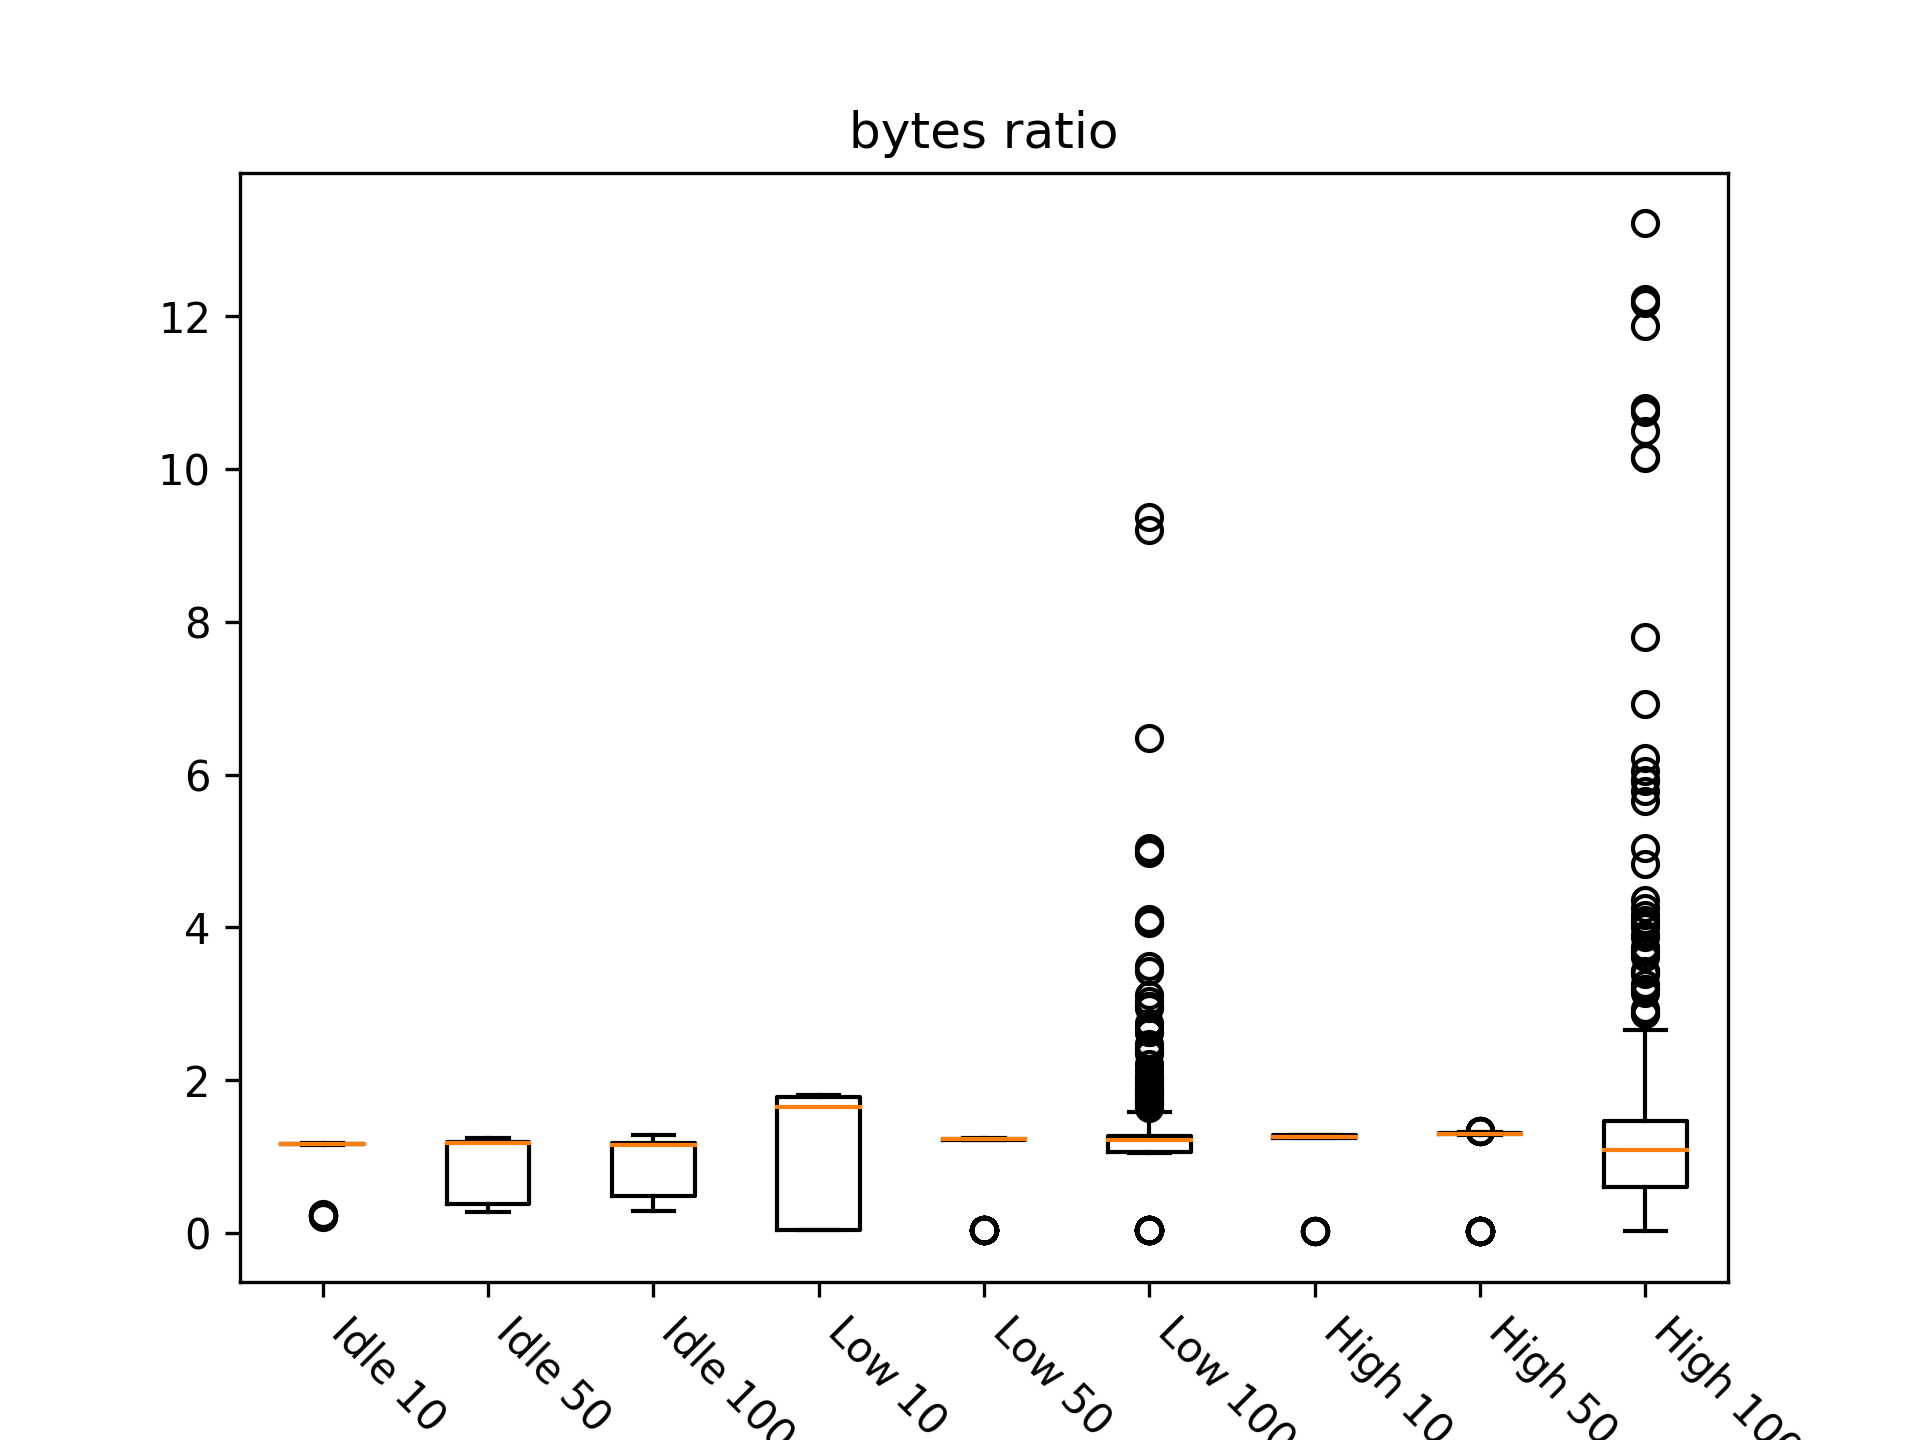
\includegraphics[width=\linewidth, height=0.4\textheight, keepaspectratio]{graphs/bytes ratio.png}
    \caption{Rapporto tra byte ricevuti ed inviati}
    \label{fig:br}
\end{figure}

\begin{figure}[H]
    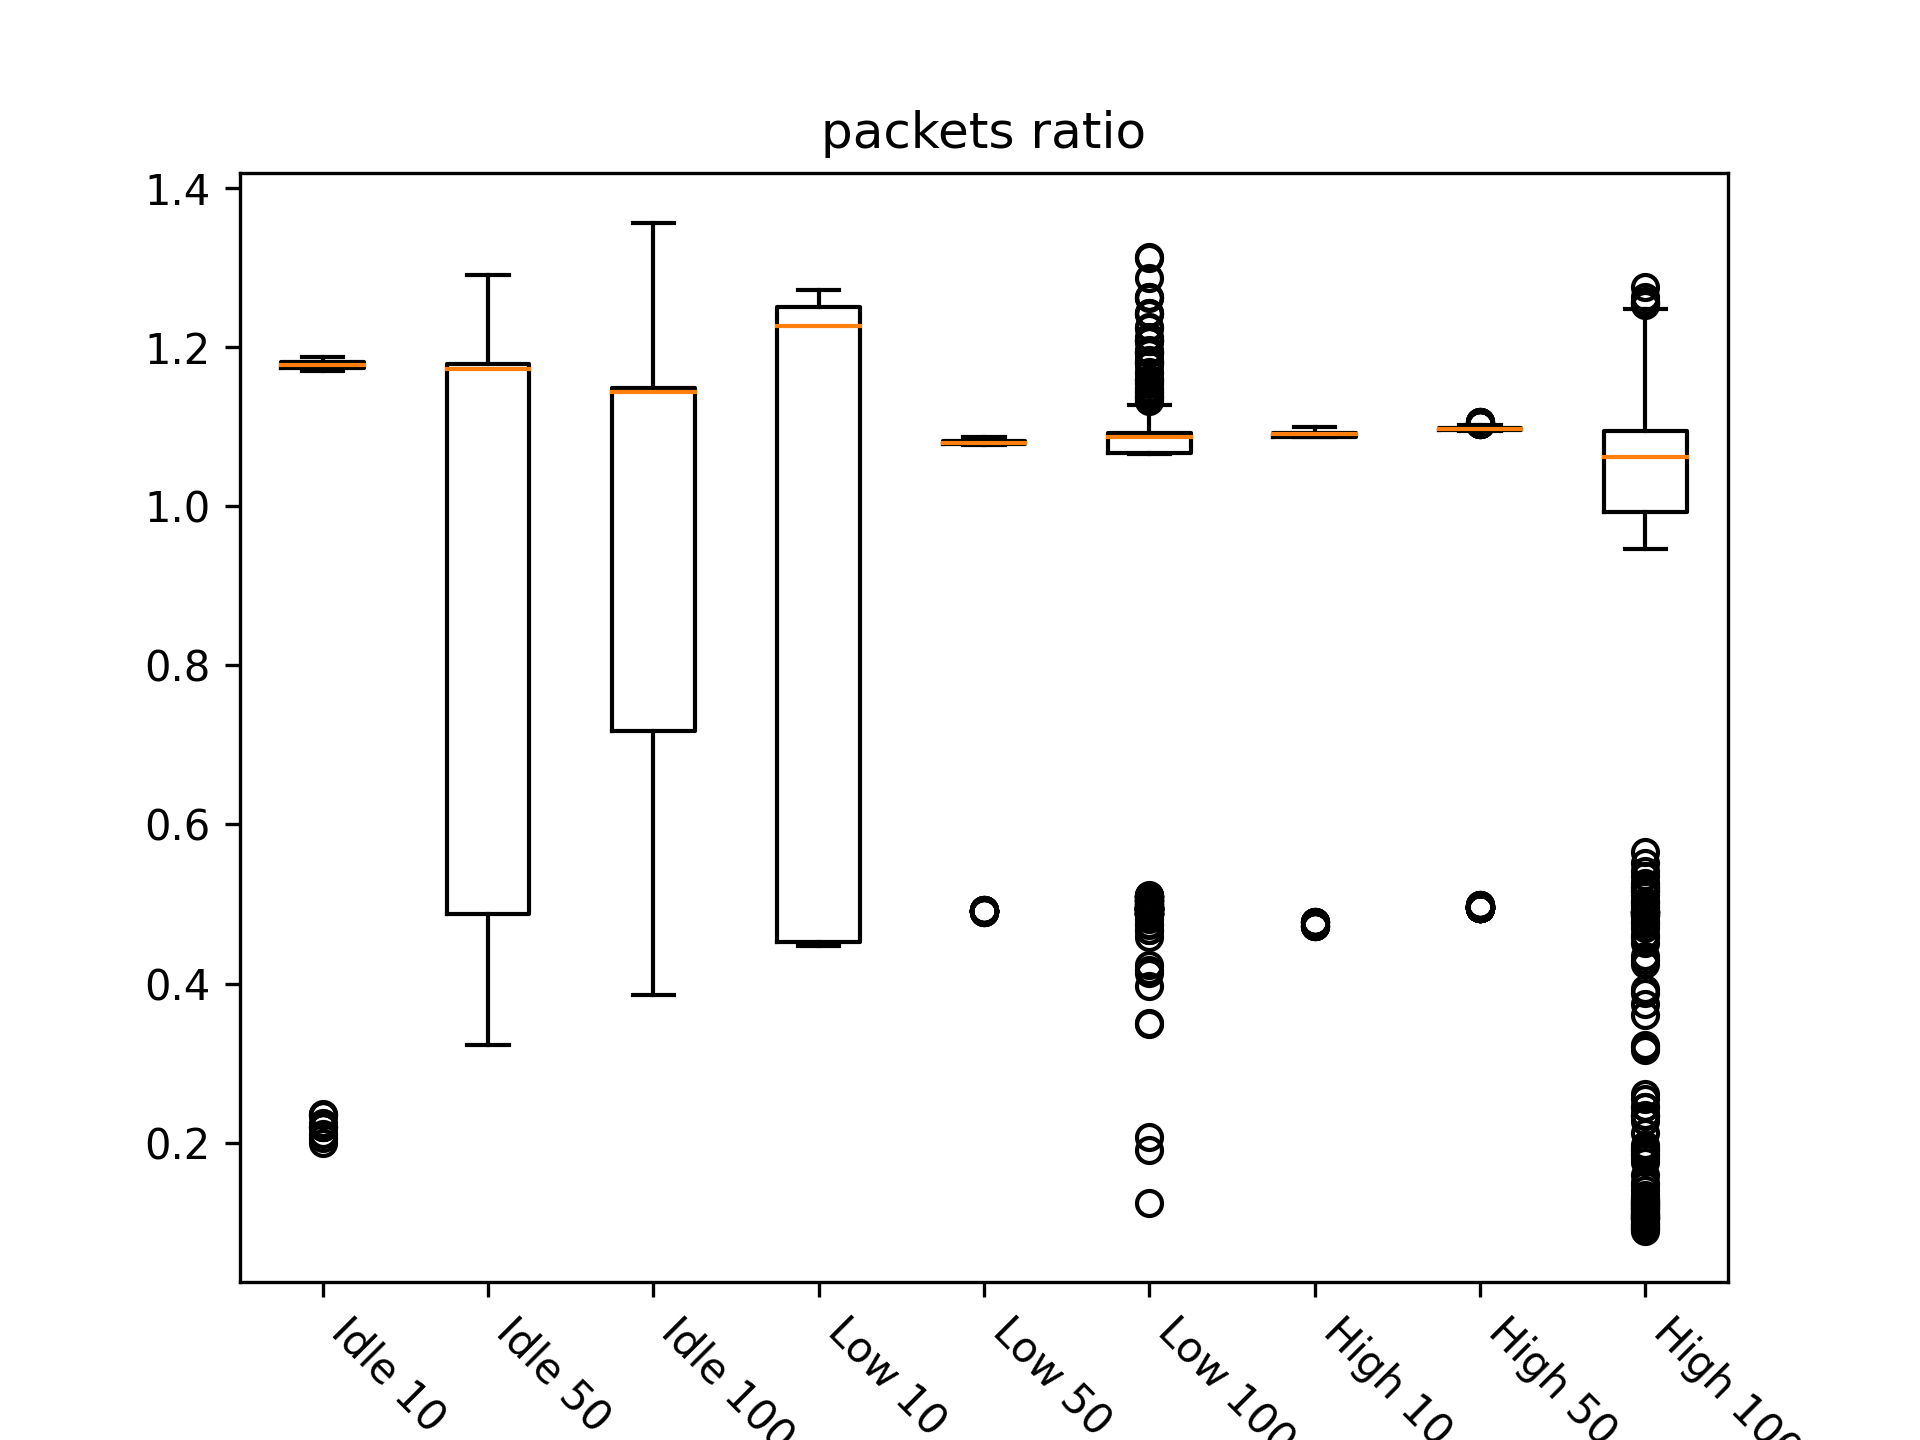
\includegraphics[width=\linewidth, height=0.4\textheight, keepaspectratio]{graphs/packets ratio.png}
    \caption{Rapporto tra pacchetti ricevuti ed inviati}
    \label{fig:pr}
\end{figure}

\begin{figure}[H]
    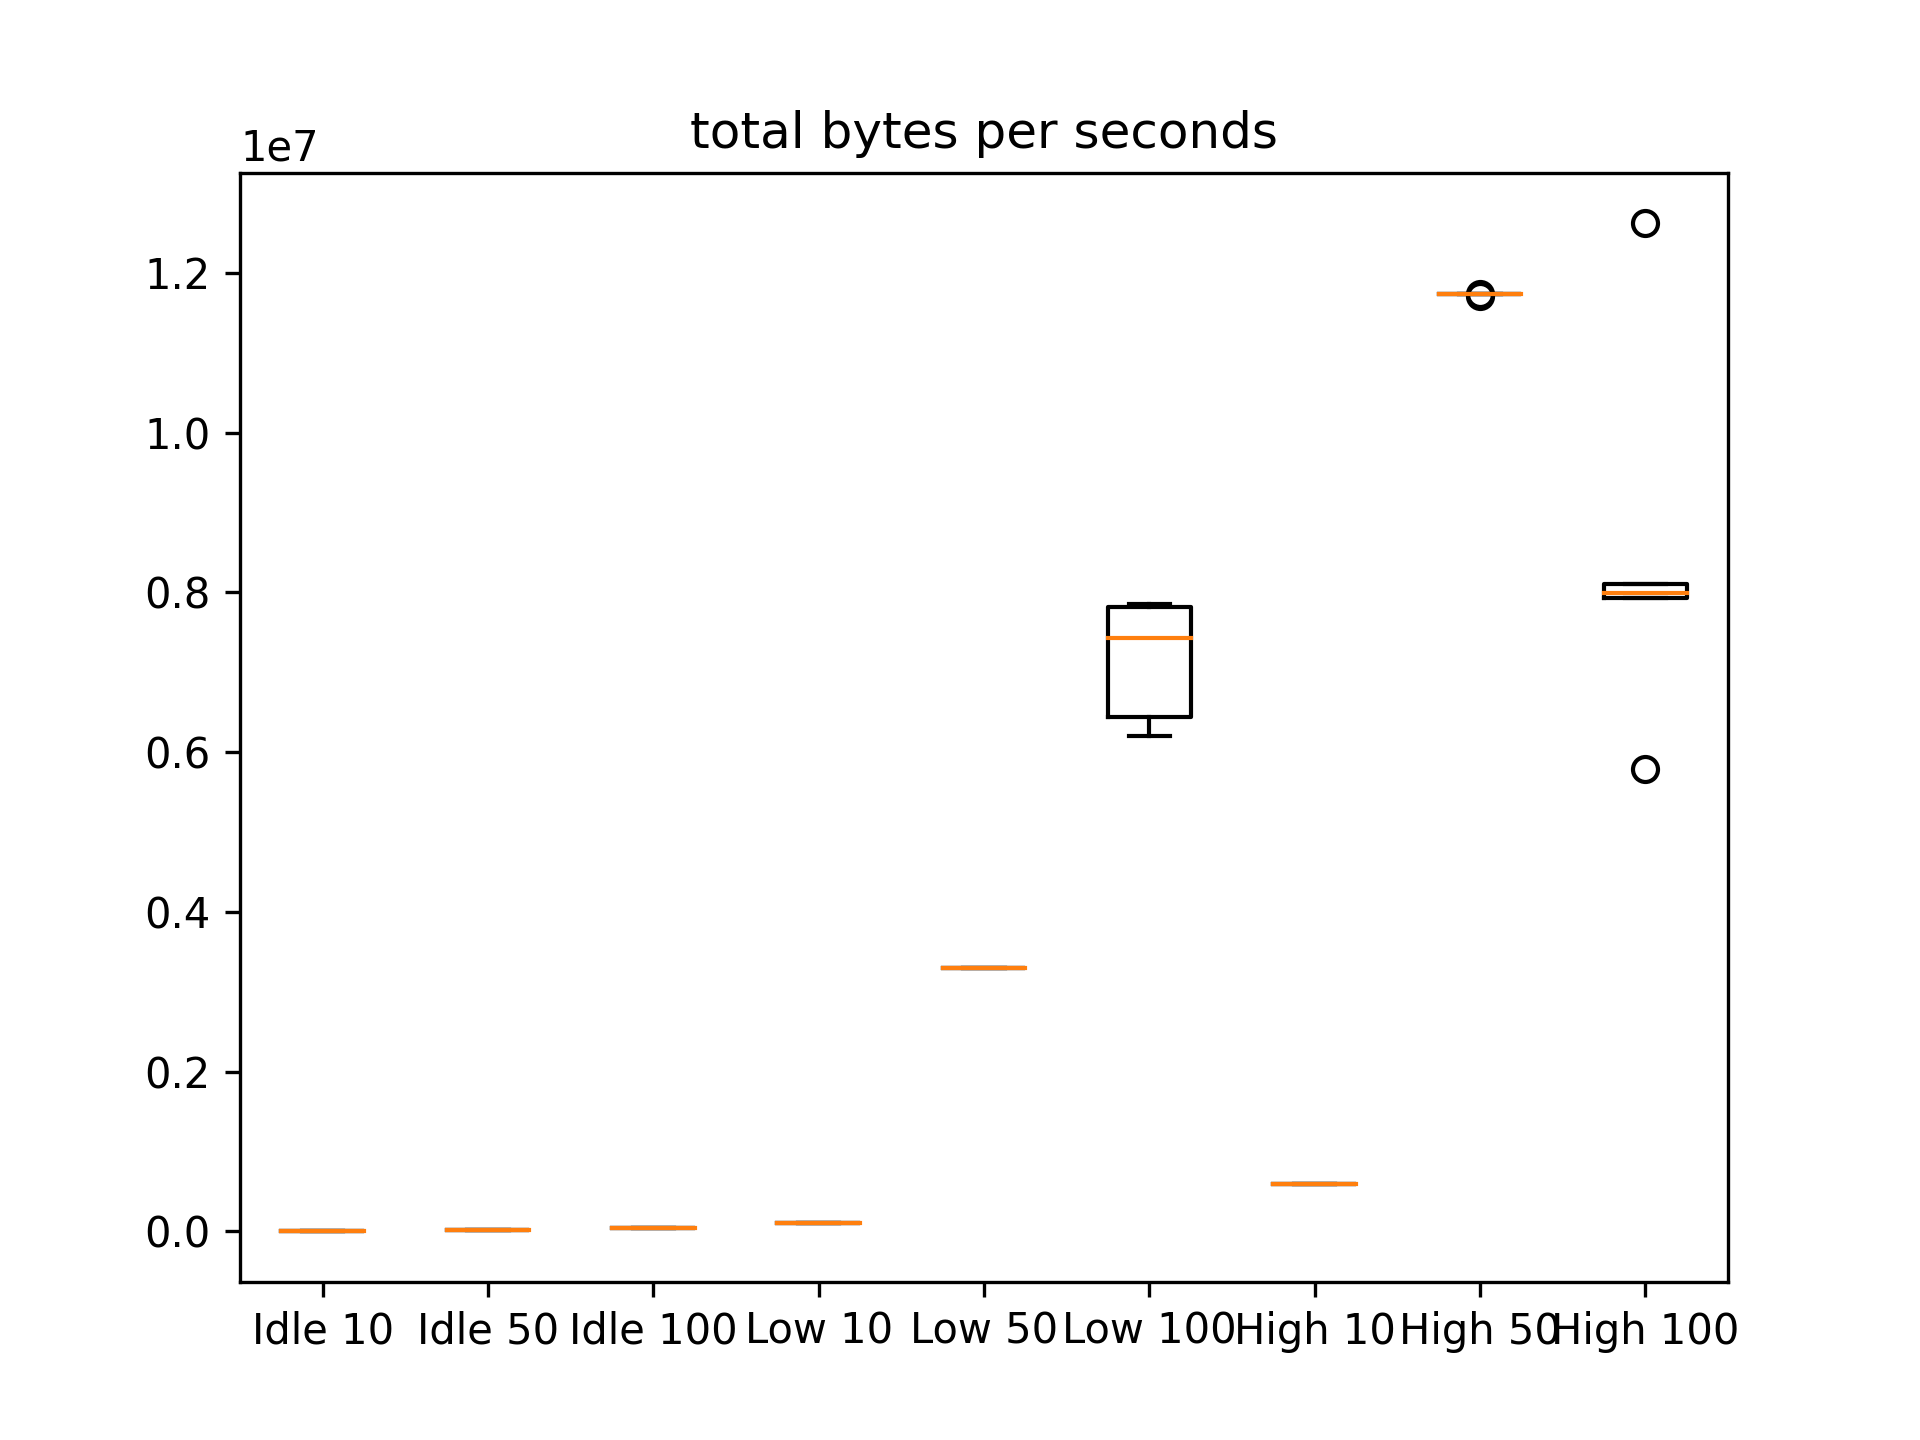
\includegraphics[width=\linewidth, height=0.4\textheight, keepaspectratio]{graphs/total bytes per seconds.png}
    \caption{Come sopra, ma diviso per la durata del test}
    \label{fig:tbps}
\end{figure}

\begin{figure}[H]
    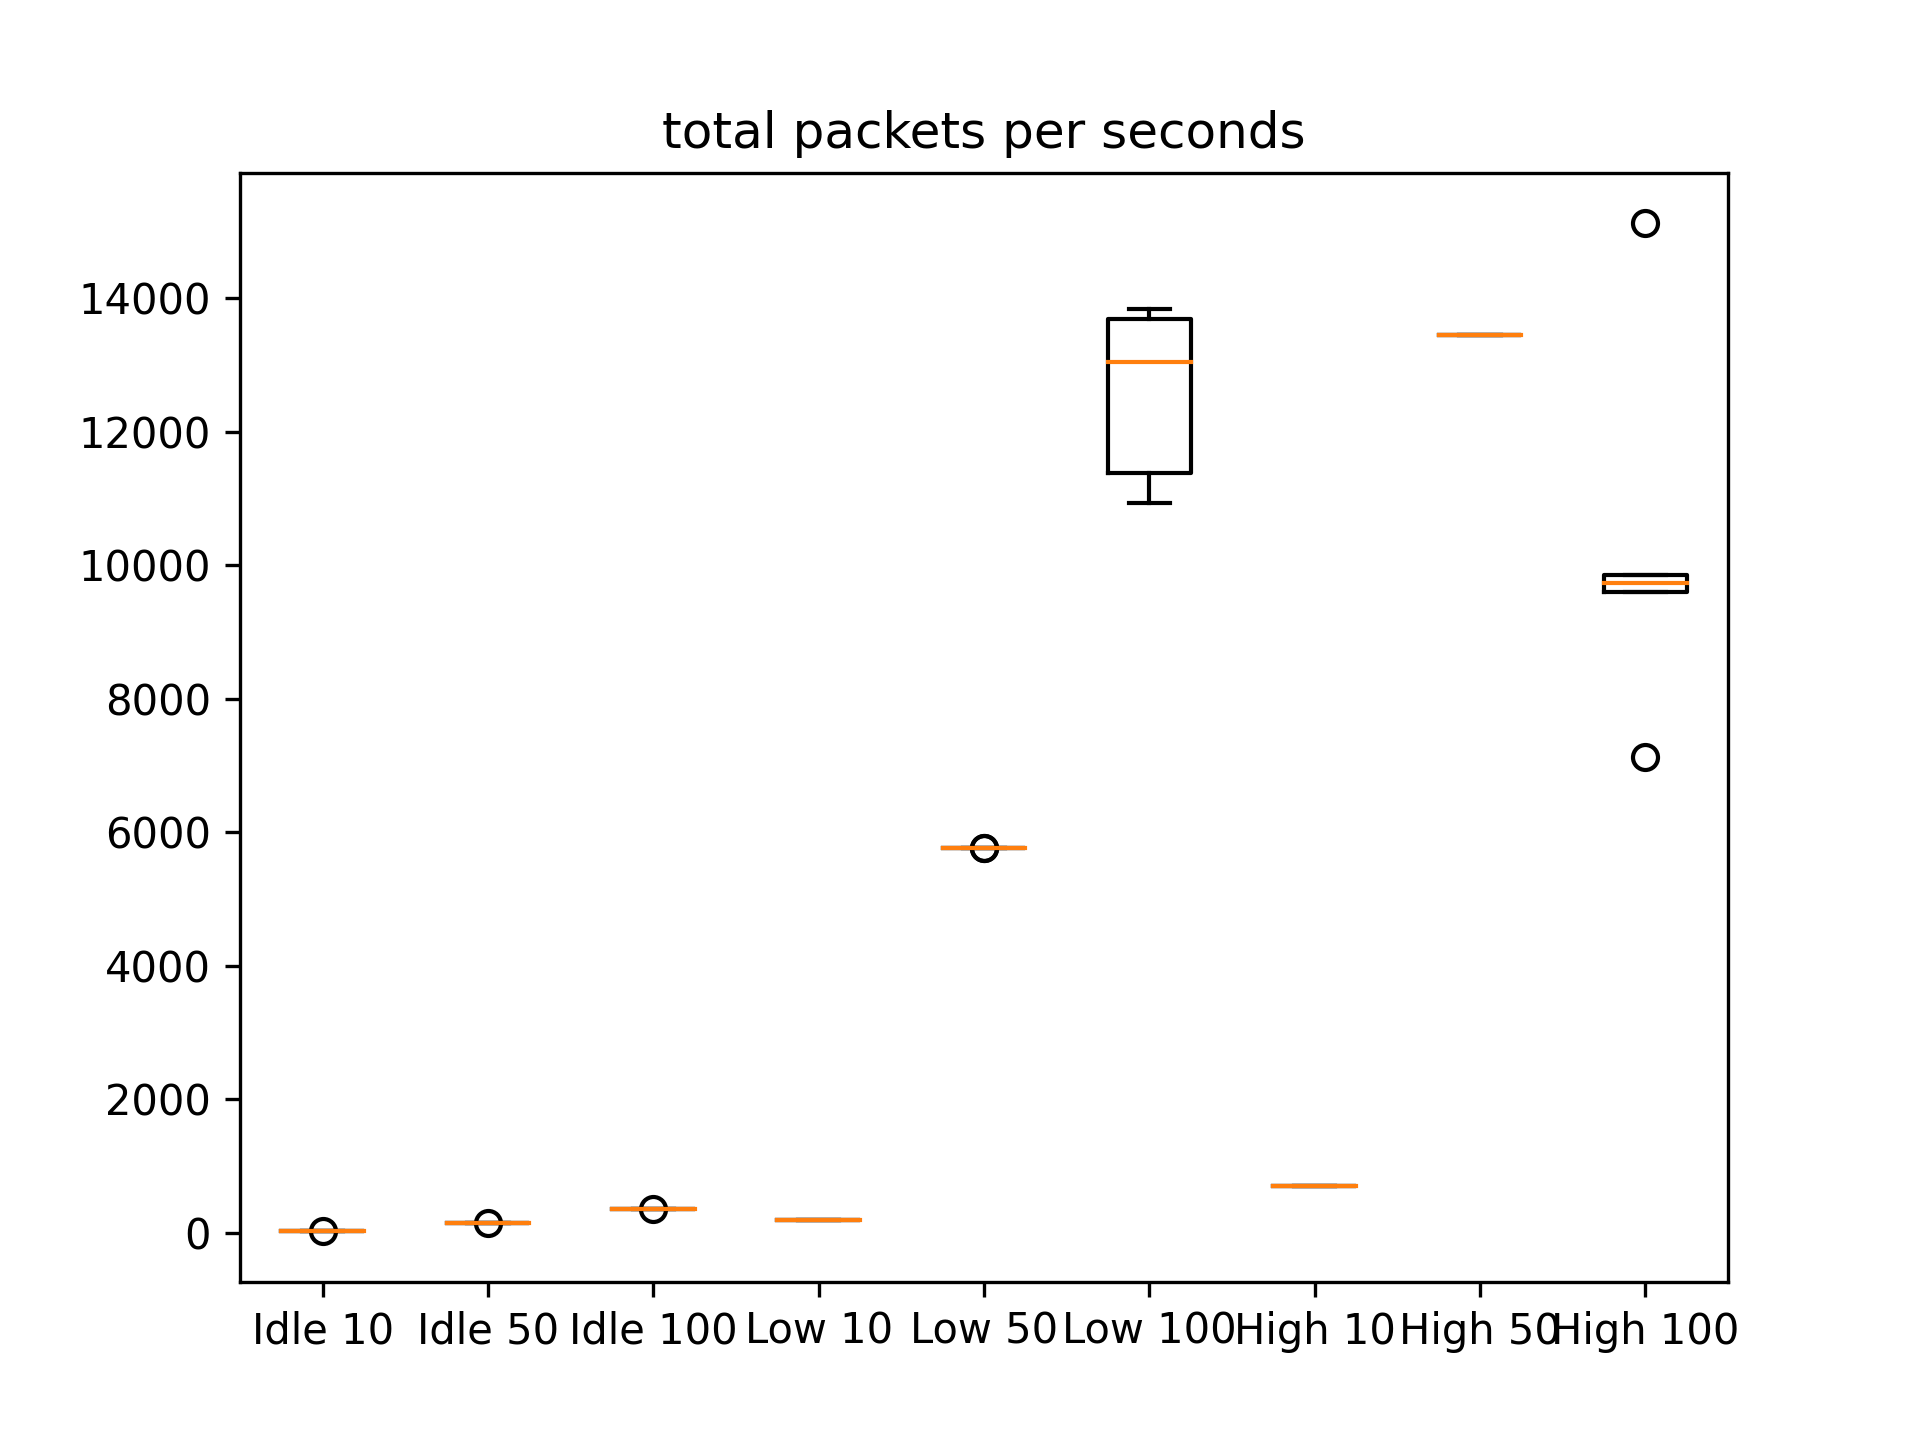
\includegraphics[width=\linewidth, height=0.4\textheight, keepaspectratio]{graphs/total packets per seconds.png}
    \caption{Come sopra, ma diviso per la durata del test}
    \label{fig:tpps}
\end{figure}

\begin{figure}[H]
    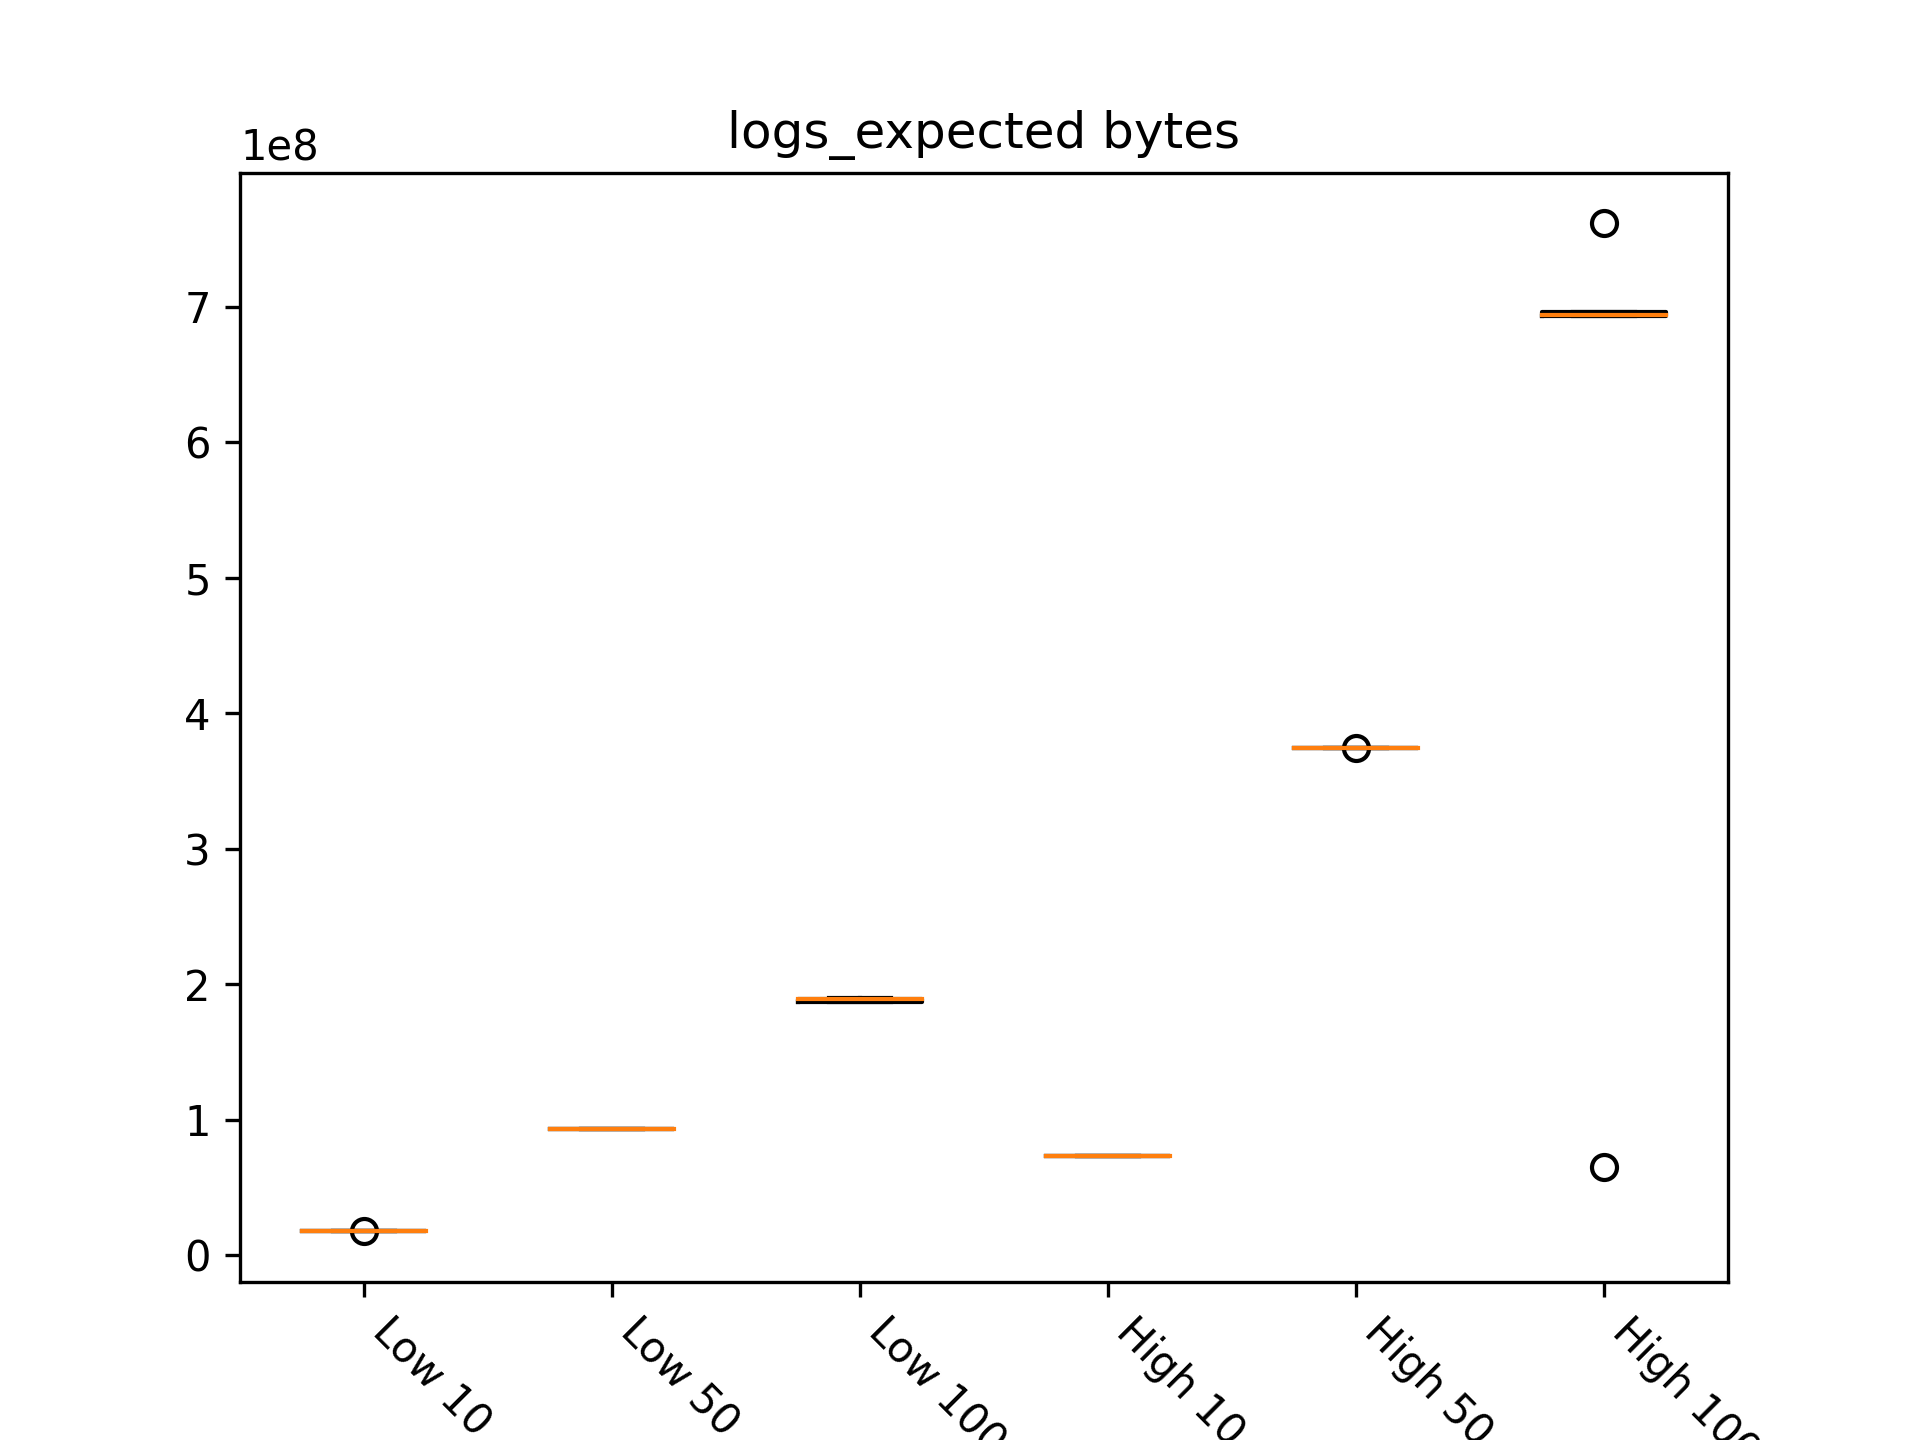
\includegraphics[width=\linewidth, height=0.4\textheight, keepaspectratio]{graphs/logs_expected bytes.png}
    \caption{Dimensione totale dei messaggi riportati nei log}
    \label{fig:leb}
\end{figure}

\begin{figure}[H]
    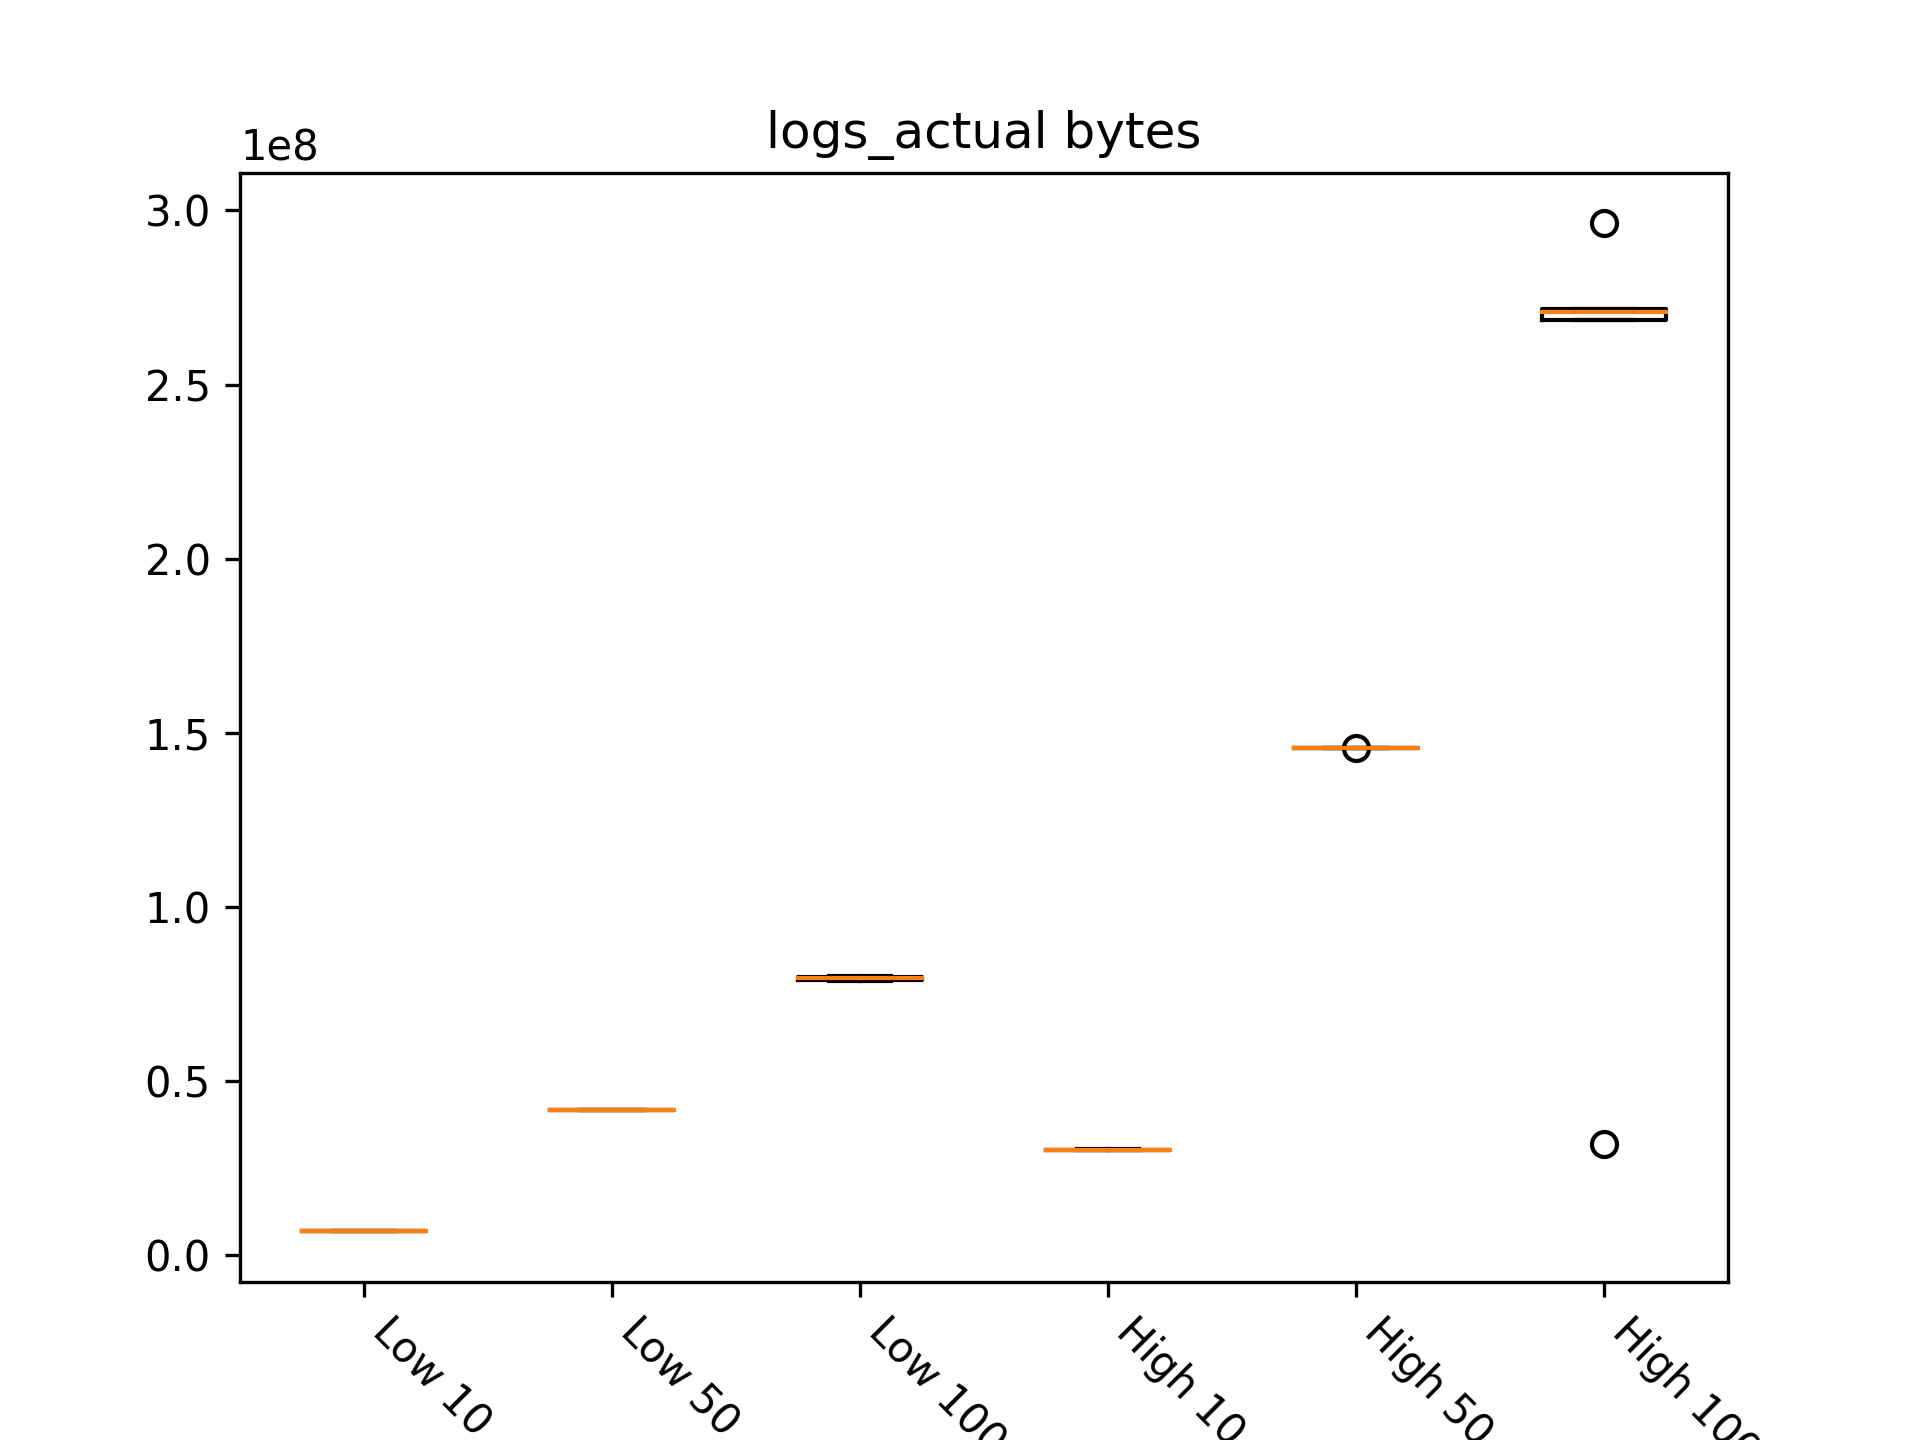
\includegraphics[width=\linewidth, height=0.4\textheight, keepaspectratio]{graphs/logs_actual bytes.png}
    \caption{Byte effettivamente inviati dal nodo loggato}
    \label{fig:lab}
\end{figure}

\begin{figure}[H]
    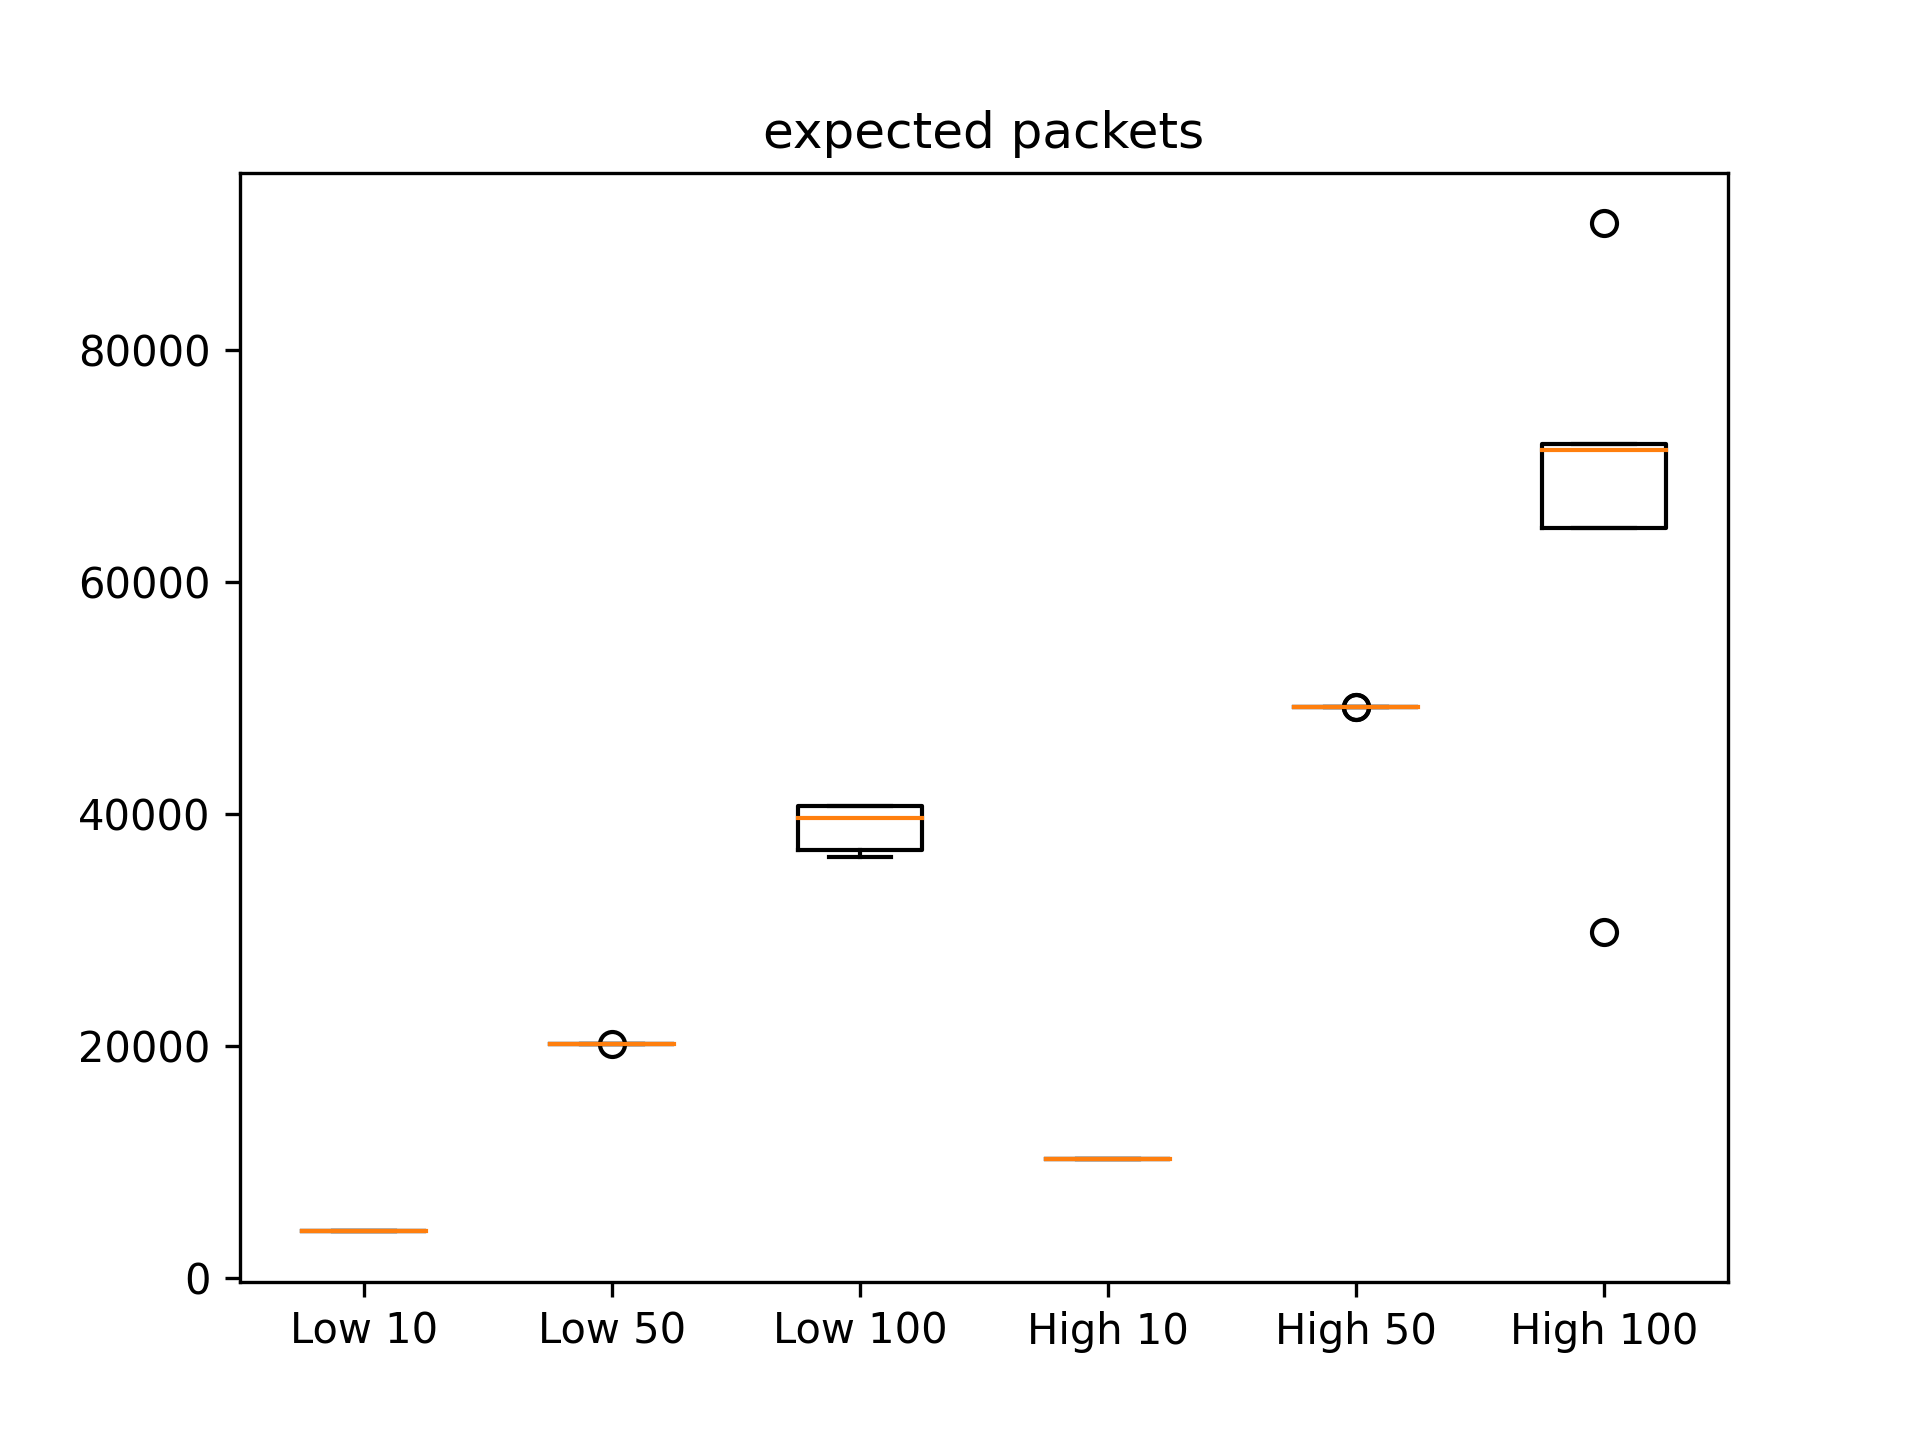
\includegraphics[width=\linewidth, height=0.4\textheight, keepaspectratio]{graphs/logs_expected packets.png}
    \caption{Numero di messaggi riportati nei log}
    \label{fig:lep}
\end{figure}

\begin{figure}[H]
    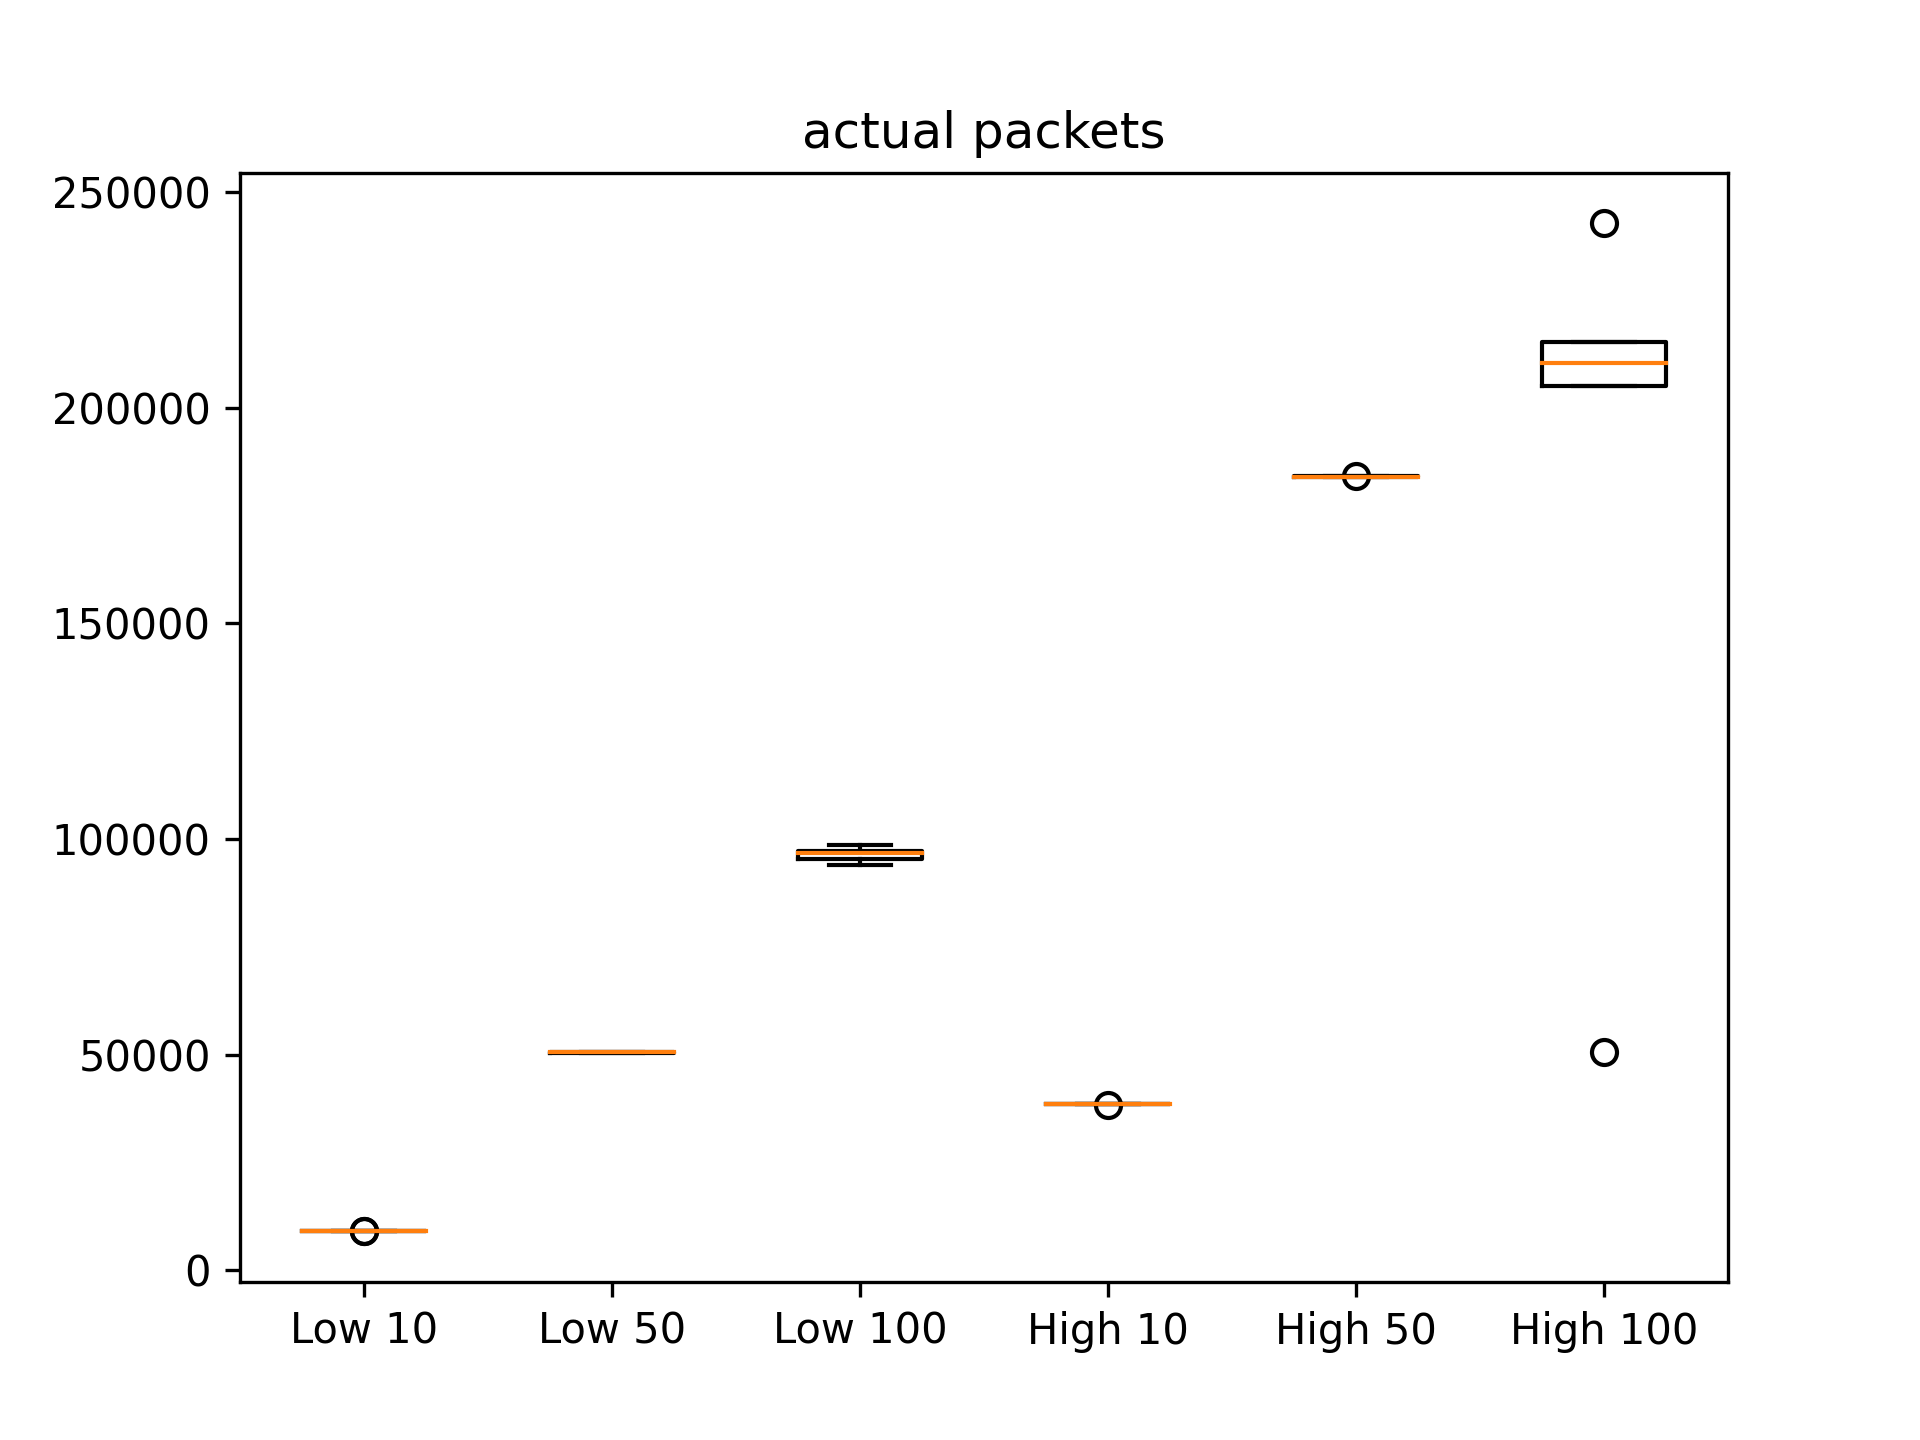
\includegraphics[width=\linewidth, height=0.4\textheight, keepaspectratio]{graphs/logs_actual packets.png}
    \caption{Pacchetti effettivamente inviati dal nodo loggato}
    \label{fig:lap}
\end{figure}

%% Parte conclusiva del documento; tipicamente per riassunto, bibliografia e/o indice analitico.
\backmatter

%% Bibliografia (praticamente obbligatoria)
\bibliographystyle{plain_\languagename}%% Carica l'omonimo file .bst, dove \languagename è la lingua attiva.
%% Nel caso in cui si usi un file .bib (consigliato)
\bibliography{thud}
%% Nel caso di bibliografia manuale, usare l'environment thebibliography.

%% Per l'indice analitico, usare il pacchetto makeidx (o analogo).

\end{document}